\documentclass[12pt]{report}
\usepackage{amsmath}
\usepackage{amssymb}
\usepackage{graphicx}
\usepackage{hyperref}
\usepackage{color}
\usepackage{float}
\begin{document}
	
	\title{Chromatin Architecture Post UVC damage}
	\maketitle
	\section{Glossary of symbols}
	\begin{itemize}
		\itemsep0em
		\item $N$- the number of monomers in the chain
		\item $d$ - dimension 
		\item $t$ - time
		\item $\Omega_(\rho)$- a sphere is $d$ -dimension with radius $\rho$ centered at the origin
		\item $D$ - diffusion constant
		\item $w$ - standard white Gaussian noise
		\item $R_i$ - position of the $i^{th}$ monomer
		\item $k_B$- the Boltzmann constant
		\item $T$- absolute temperature
		\item $\xi$- friction parameter
		\item $b$- the standard deviation of the distance betwen neighboring monomers
		\item $l_0$- the minimal allowed spring length
		
	\end{itemize}
	\section{Experimental Settings and Main Findings}
	\begin{enumerate}
		\itemsep0em
		\item Cell type used: U20S, which are human osteosarcoma cells;
		\item H3.3 histones are tagged 48 hours before experiments using the SNAP-tag method, tag color is red;
		\item Repair factors XFP are labeled with GFP;
		\item A region of $20 \mu m^2$ was photo-activated 8-10 hours before UVC;
		\item UVC damage is induced in a region of the cell using a 266 $nm$ laser (0.266 $\mu m$);
		\item Changed to the red fluorescence signal were measured in the entire volume of the cell, post UVC;
		\item Images were acquired using confocal microscopy, with an auto-focus module on, to acquire images from the best focal plane;
		\item Fluorescence intensity were normalized against values measured in undamaged nucleus;
		\item Fluorescence loss at irradiated sites was determined by dividing the intensity in the illuminated area by the intensity of the entire nucleus after background subtraction;
		\item Illuminated area was defined 15 minutes post UVC based on GFP labeled repair factors and was kept similar throughout measurements;
		\item Fluorescent recovery was measured relative to previous illumination starting from the frame with the minimal fluorescent values;
		\item 2D projection of the 3D images were obtained by \textit{maximal intensity z projection};
		\item To gain sensitivity, most of the cell H3.3 fluorescence was photo-bleached, aside from the region of UVC illumination;
		\item 20\% loss of H3.3 signal from the \textit{entire nucleus} was detected after photo-bleaching the fluorescence patch;
		\item However, using UVC in the fluorescent patch led to 40\% loss of parental H3.3 signal, while no detectable loss was seen in the entire nucleus;
		\item The depletion of fluorescence signal in the center of the damage area, 15 minutes post UVC, was accompanied by an increase of density at its boundaries, balancing the loss;
		\item 20\% loss of DNA signal in the damage region, accompanied by an expansion of the region was observed 15 minutes post UVC;
		\item The expansion of the damage region depends on the dose of repair-factor;		
		\item The early repair factor DDB2 recruits histone chaperons HIRA, which promotes the deposition of newly synthesized histones at UVC sites;
		\item newly synthesized histones are detectable in the repair region only 45 minutes post UVC;
		\item Histone chaperons do not participate in histone redistribution after UVC irradiation;
		
	\end{enumerate}
	
	
	\section{Model and Parameter Estimation}

	\subsection{Simulation outline and definitions}
	We perform 3 stage simulation: 
	\begin{itemize}
		\itemsep0em
		\item recording stage;
		\item repair stage - in which a UVC beam is shot at initiation;
		\item post repair stage
    \end{itemize}
    
	\subsection{Nucleus Size}
	 Cells' cross-section are 240 $\mu m^2$ in the $x-y$ plane and $11 \mu m$ in height, giving an average radius of $r_c=7.25 \mu m$.  
		
	\subsection{The Simulation Domain}
	We set our simulation in a spherical domain with reflecting boundaries. The circle, $\Omega_d(\rho)$ of radius $\rho$, will represent a region around the damage site, rather than the entire nucleus. 
	because the UVC beam is shot vertically through the cell, every layer in the 3D is damaged equally. We consider the process of DNA dynamics post UVC to be similar in each 3D stack and perform our experiment in 2D, which simulates the Z-projection made in the experiments.
	To keep the polymer dense inside this region, we set $\rho=(b\sqrt{N/6})/2$. The actual value of this parameter is yet to be justified. The reflecting boundaries mimic the condensation barrier of the DNA with surrounding chromosomal chain, unaffected by the UV damage. 
	\subsection{The chromatin [to be corrected]}	
		The chromatin is modeled as a monomer-spring polymer of $N$ monomers connected by harmonic springs. The dynamics of the polymer is governed by 3 forces: thermal fluctuations, spring force, and bending force, which we vary during simulations to approximate the observed experimental behavior. Before UVC beam is shot, the polymer's dynamics is governed by spring forces only, whereas after UVC the affected monomers of the chain along with their nearest neighbors are assigned additional bending elasticity forces. 
		
		Thermal diffusion fluctuation, results from the random collision of the polymer with the particles of its surrounding, and is given by 
		\begin{equation*}
		F_d(t) = \sqrt{2D}\frac{dw}{dt}
		\end{equation*}
		with $D$ the diffusion constant, defined by $\frac{k_BT}{\xi}$, $k_B$- the Boltzmann constant, $T$- the absolute temperature in Kelvin, $\xi$-the friction coefficient, and $w$ is a standard white Gaussian noise. 
		
		The spring force, derived from an harmonic potential of springs connecting neighboring monomers, is given by
		\begin{equation*}
		F_e(t) = -\gamma_e\frac{dk_BT}{2b^2}\frac{\partial}{\partial R_n}\sum_{n-1}^{N-1}(|R_n(t)-R_{n+1}(t)| -l_0)^2
		\end{equation*}
		with $\gamma_e>0$ spring constant,$d$ is the dimension, $b$- the standard deviation of the distance between monomers, $R_n(t)$ is the 3D position of the $n^{th}$ monomer at time $t$, and $l_0$ is the minimal allowed distance between neighboring monomers.
		
		Bending force on the $n^{th}$ monomer is defined in terms of the angles $\theta_i$ between three adjacent monomers of the chain, $n,n+1,n+2$;
		\begin{equation*}
		F_b(R_n) = -\gamma_b\frac{dk_BT}{2b^2}\frac{\partial}{\partial R_n}\sum_{i=1}^{N-2}(\cos(\theta_i(t))-\cos(\theta_0))^2
		\end{equation*}
		
		The differential equation describing of motion of the chain is thus 
		\begin{equation*}
		\frac{dR_n(t)}{dt}= F_e +F_b +\sqrt{2D} \frac{dw}{dt}     
		\end{equation*}
					
	\subsection{The UV beam}
	UV beam has 3 $\mu m^2$ section, yielding a radius of $r_{uv}=\sqrt{\frac{3}{\pi}}\approx 1 \mu m$. 
    The damage cause by the UV beam follows a Gaussian distribution around the UV beam focus. In simulations, we place the focus of the beam on the polymer's center-of-mass, and activate it once, evaluating for each monomer within the beam's area the probability to be damaged. [Insert here the experimental data]
    
	\begin{figure}[H]
	\centering
	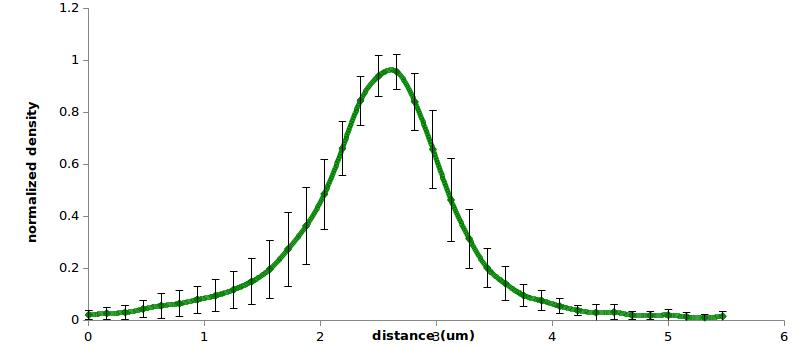
\includegraphics[width=0.45\linewidth, height=0.2\textheight]{UVDamageDistribution}
	\caption{\tiny{\textbf{Distribution of damaged site, average of two experiments. the distribution follows roughly a Gaussian distribution with parameter 1.5}}}
	\label{fig:UVDamageDistribution}
	\end{figure}
	
    In line with experimental measurement, the probability of a monomer to be damaged follows a Gaussian distribution with its center at the UVC beam's center-of-mass, which is placed at the polymer's center-of-mass. Only monomers found within the UVC beam area are tested to be damaged. 
      	
    \subsection{UVC effect on monomers}
      Several scenarios will be examined in this report:
      \begin{enumerate}
      	\itemsep0em
      	\item We assign bending elasticity to damaged monomers, with an opening angle $\theta$;
      	\item We assign bending elasticity to the non-damaged monomers with an opening angle $\theta$;
      	\item We assign bending elasticity to the non-damaged monomers found only in the UVC beam and unaffected by it, with opening angle $\theta$;
      	\item We create a region of exclusion around each damaged monomer of radius $r_e$ with an harmonic pushing force.
      \end{enumerate}
      In the case of bending force, we will assign bending elasticity to damaged monomers and their nearest neighbors. This is done to create a polymer segment containing at least two monomers for the force to act upon and to prevent non ordinary behavior of isolated monomers assigned bending elasticity.      
	
	\subsection{The region of interest (ROI)}
     The area of chromatin expanded after UVC occupies $10 \mu m^2$ which gives 3 times the UVC beam radius, i.e. $3\mu m$, but is generally dependent on the intensity of the UVC beam and recruitment of repair proteins. 
     The region of interest (ROI) in experiment is determined by the presence of the repair mechanism 10-15 minutes post UVC. Repair proteins are thought to be bounded to damaged section of the chromatin. Accordingly, we define the ROI as the radius of expansion, $\rho_e$, of the damaged monomers at the end of repair stage and remains of fixed size. The radius of expansion is defined as the mean square distance of 90\% of the damaged monomers from their center of mass. 
     The center of the ROI is dynamically placed at the center of the mass of the polymer at each step. All density calculation within the ROI are made off-line. 
	
	\subsection{DNA density}
    We evaluate two quantities within the ROI related to the density of the chromatin within it. The first, we calculate the number of monomers (vertexes) located within the ROI at any given step. The second, we calculate the total length of bonds falling within the circular ROI.
	
    \subsection{Histone Density}
		We consider histones to be uniformly distributed in the nucleus and in the damage zone. There are $3\times 10^6$ histones marked, which makes their density $3\times 10^6 /(4 \pi 7.25^3)\approx 630$ histones/$\mu m^3$
		The expected number of histones in the UV beam region is $14.5\pi \times 630\approx 30,000$ histones, assuming the beam is shot through the center of the sphere. 
		
		histone density in simulations [To be Determined]
        						         
    \subsection{Model Parameters}
      Parameters used in simulations are set proportional to of the quantity $\frac{dk_BT}{b^2}$, which we fix to be 1 by setting the friction factor $\xi=1$. 
    \subsubsection{The parameter b} 
      we set $b=\sqrt{dimension} \times 100 nm$, 
    \subsection{The minimal distance between monomers -$l_0$}
     We set $l_0$ to be $\sqrt{d}$ to match $b$ and allow fast relaxation of the chain configuration before UVC beam shot, after diffusion is turned off. 
    \subsubsection{Number of monomers}
      The number of monomers, $N$, is determined by setting the polymer's radius of gyration to covers the ROI. The radius of gyration is given by $\sqrt{N/6}b$, equating it to $3\mu m$ we get $N\approx 1800$                      
     \subsubsection{The Spring constant}
       We set the spring constant $\gamma_s =1$
     \subsubsection{The bending constant}       
       The bending constant affects the rate at which the polymer assumes new conformation after UVC damage.
       We set it to be proportional to the bending constant, as $\gamma_b frac{3K_bT}{b^2}$. later we will adjust this constant according to the rate of chromatin expansion seen in experimental data. 
                   
    \subsection{The ROI}
    The circular region of interest (ROI), in which we calculate monomer densities gain and loss, is determined according to the expansion of the damaged monomers.
    We set the percentage of included damaged monomers to 95\%. The ROI is calculated from the polymer's center-of-mass, such that 95\% of the damaged monomers are included within it. 
    The ROI is calculated at the end of the repair phase, after expansion has thought to reach saturation [How is saturation determined?]. The radius of the ROI is then used to back-calculate the densities within it relative to the center of mass of the polymer at any time step starting from the beam shot time. 
    
    \subsubsection{determining expansion saturation}
     In the current version of the simulation framework, we assume the expansion of the affected monomers has reached saturation at the end of repair phase. To determine the radius of the ROI, we take the average of the affected monomers' radius of expansion in the last 10\% of the steps in the repair phase. 

    		             		
	\section{Simulations}	
	
	\subsection{Simulation procedure}
	Simulations were ran $numRelaxationSteps$ up to relaxation, after which the diffusion force was set to $0$ and recording for $numRecordingSteps$. Following, the UV beam was shot through the center of the polymer's mass. Monomers found within the UV beam area were considered damaged with a probability following a Gaussian distribution (as provided by the experimental data). Simulation were then ran for additional $numBeamSteps$.
	
	Simulation were placed in a spherical domain with reflecting boundaries.
	Measurement of density were performed on a circular region, with its center dynamically placed at the polymer's center-of-mass, and it's radius determined at the end of the repair phase by the radius of expansion of the damaged monomers.
	Sizes of the containing sphere (circle in 2d) and the measurement region were proportional to the radius of gyration, $\sqrt{N/6}b$.
	

	  
	\section{2D simulations of DNA loss}
	 
	\subsection{Adding Lennard-Jones force}
      After UVC, several monomers are hit and together with their nearest-neighbors are assigned bending elasticity with an opening angle of a certain value. Usually, a region of consecutive affected monomers is enclosed by non-affected monomers. Therefore, the result of activating the bending elasticity force for the affected monomers is the formation of horse-show type of loops structures. 
      Affected monomers are located at the center of the polymer and expand usually outwards (although the direction of expansion cannot be controlled). The problem is that the expanded region of the chain exit the ROI and keep expanding passed the layer of non-affected monomers, that are usually located outside the ROI. 
      
      The Rouse polymer permits bonds to cross each other, and therefore the affected monomers do not stop at the non-damaged monomer layer. 
      to try to confine the damaged monomers to the region of the damage, we assign volume exclusion, Lennard-Jones potential, to the chain. The non-affected monomers will hopefully counter-balance the expansion of the damaged monomers, keeping them from passing the non-affected layer outside the damage zone.
      
      In the experiments explained below we ran the simulation to see if the radius of expansion of the damaged monomers can be limited by the Lennard-Jones fores. Simulations are performed in two-dimensional spherical environment, the polymer includes 500 monomers.      
      
     \begin{figure}[H]
     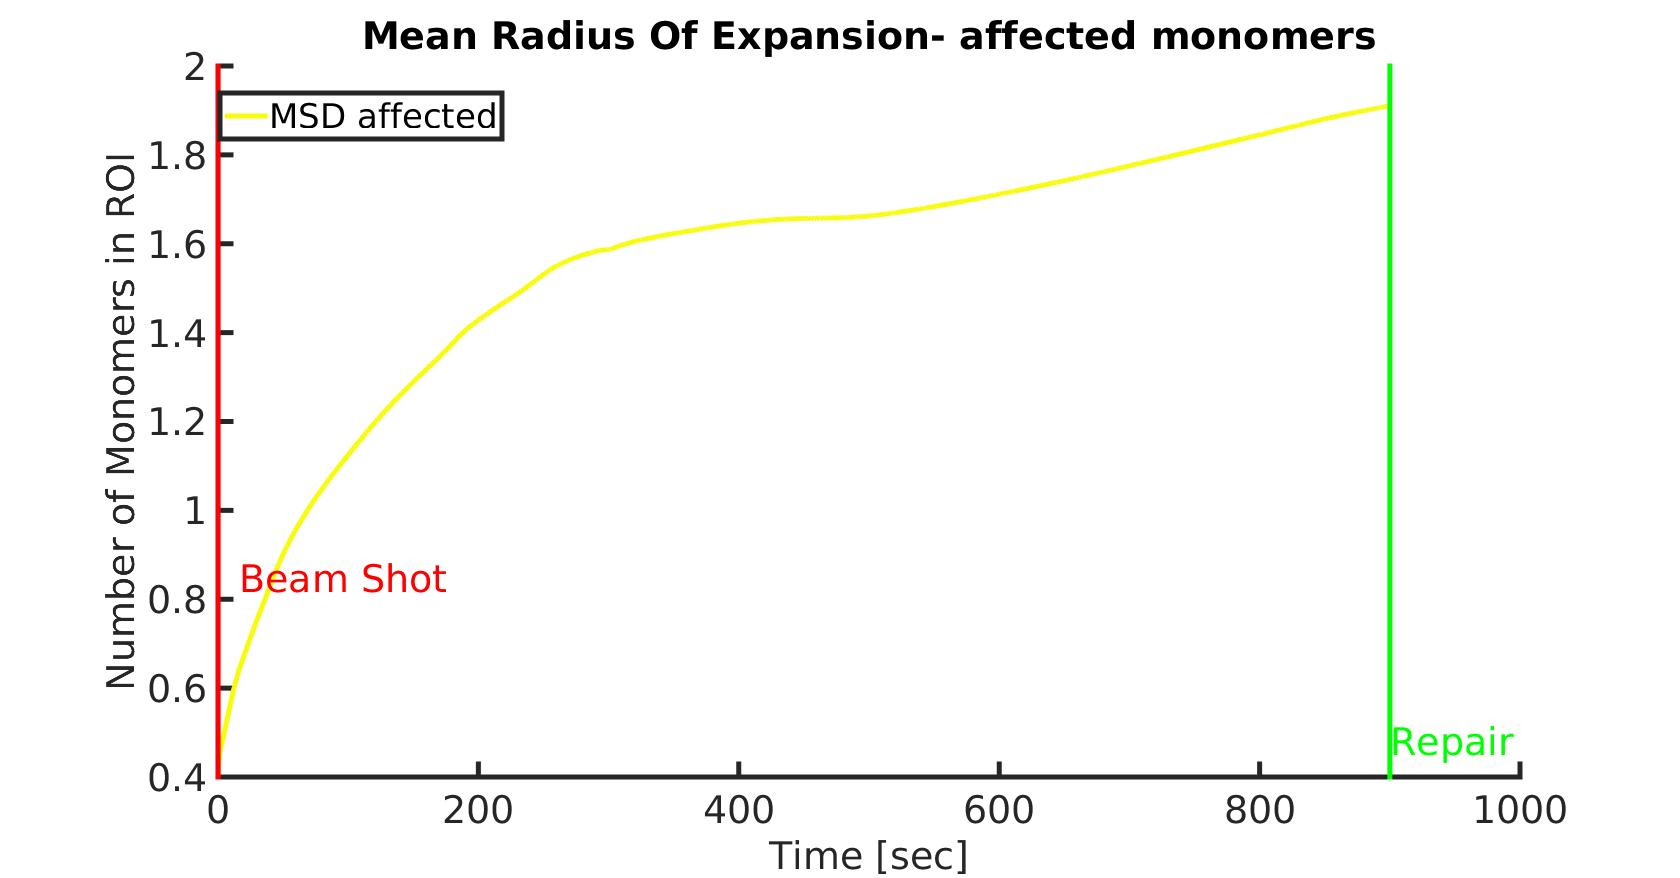
\includegraphics[width=0.5\linewidth, height=0.3\textheight]{RadiusOfExpansion500BeadsLennardJones}
    	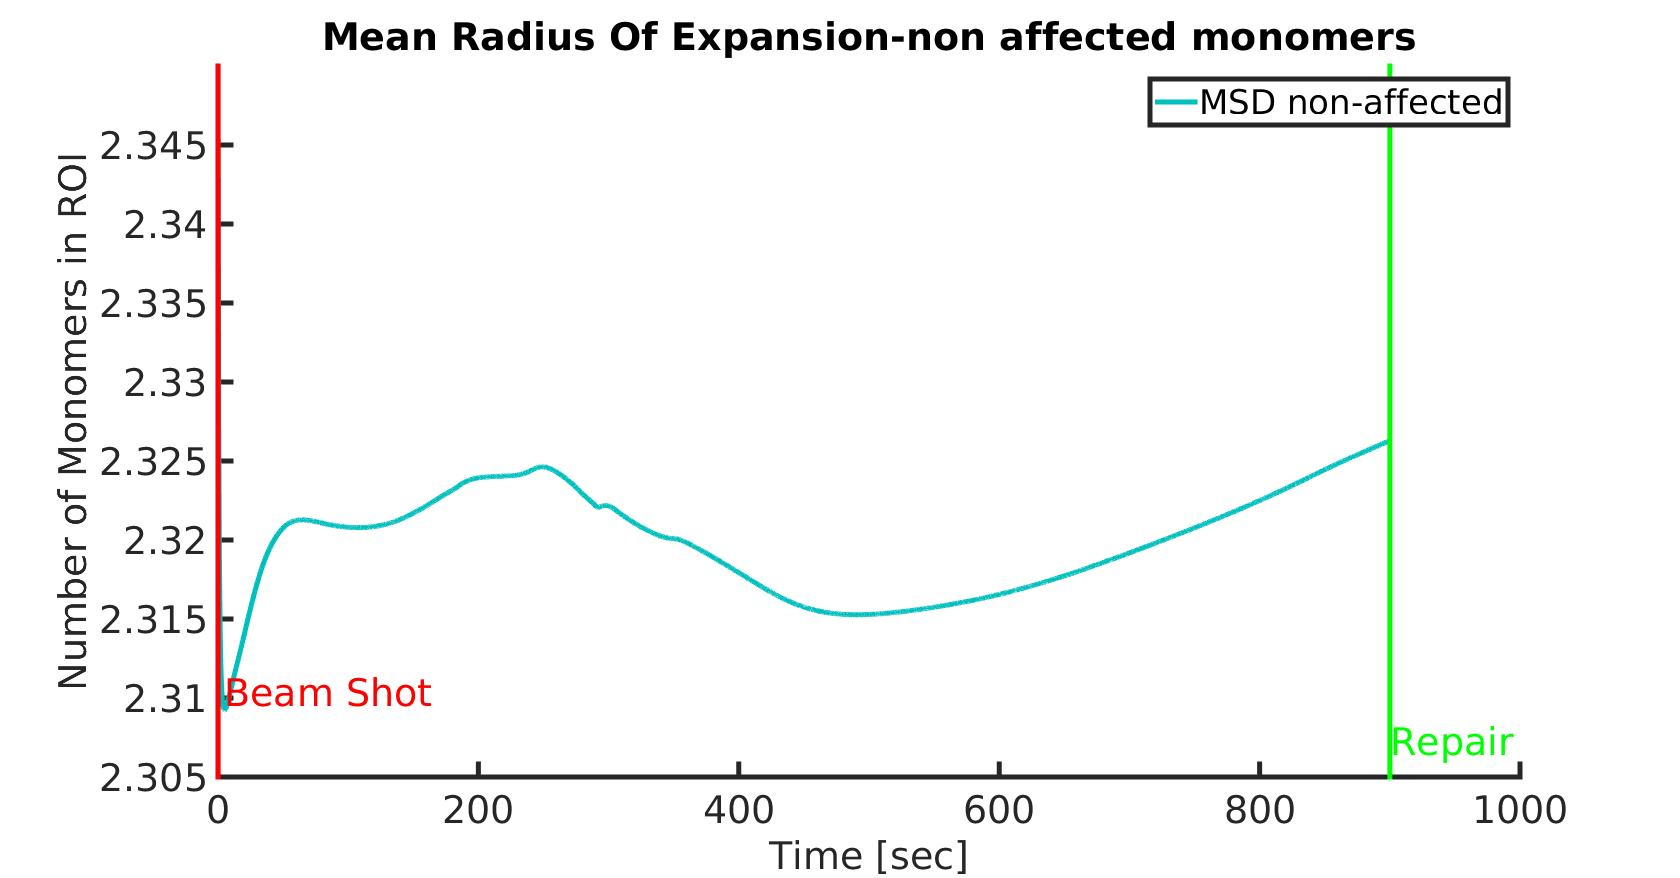
\includegraphics[width=0.5\linewidth, height=0.3\textheight]{RadiusOfExpansion500BeadsNonAffectedLennardJones}
        \caption{Radius of expansion relative to the monomers' center-of-mass, for the damaged (left) and non-damaged (right) monomers of the chain.(Mean of 5 experiments of 9000 steps each, polymers contain 500 monomers)}
        \label{fig:RadiusOfExpansion500BeadsLennardJones}
      \end{figure}
      
      From figure \ref{fig:RadiusOfExpansion500BeadsLennardJones} we can see that the Lennard-Jones is not sufficient to stop the monomers from expanding. The damaged monomers' MSD in relation to their center-of-mass keeps increasing until about 300 sec, where it reaches a local plateau. At this point, many damaged monomers are at the same distance as the non-damaged ones and the expansion seems to go into a halt. Once the bending force overcomes the resistance by the Lennard Jones force, the expansion continues. The damaged monomers' radius of expansion doesn't reach the value of the non-damaged. However, we suspect that it will, given enough time for simulation. Moreover, the expansion is measured relative to the center-of-mass of either the damaged or non-damaged, and so it is not clear where are those two groups relative to each other. 
      
      Changing the radius of expansion to be calculated relatively to a fixed point, namely the beam's center at initiation, does not change the magnitude of expansion. The damaged monomers keep-on expanding. 
      
      We therefore, omit the Lennard-Jones potential from further consideration in the next simulation.


   \subsection{Cross-linking the polymer}
    To prevent monomers from expanding after UVC in an uncontrolled manner, we randomly add connectors between pairs of non-nearest-neighbor monomers in addition to the linear backbone of the polymer. The measure for connectivity we use is the percentage of connected pairs out of the total number of monomers, e.g. 50\% connectivity in a 100 monomer chain corresponds to 25 additional connector (connecting 50 monomers). 
	
	At simulation initiation, we let the polymer relax to a state in which the cross-linked monomers are brought into proximity according to the minimal allowed distance. After UVC beam shot, we divide our results into two parts. In the first, we assign bending potential to the damaged monomers, in the second we assign bending potential to the non-damaged monomers. We further divide each case into two scenarios according to the effect of UVC. In the first, we break all damaged cross-links, that is, a connector to any affected monomers. In the second, we keep all cross-links throughout the simulation. 
	In all simulation,the ROI was determined according to the damaged monomers radius of expansion.
	
	\subsection{Assigning bending to damaged monomers}
	In this simulation we add bending elasticity potential to damaged monomers and their nearest-neighbor. Assigning bending potential to the damaged monomers' nearest neighbor was done to prevent peculiar dynamics isolated damaged monomers had and to create a more continuous regions affected by bending due to damage. The ROI is determined by the expansion of the damaged monomers. 
	
	\subsubsection{Break damaged monomers' cross-links}
	After UVC we break all cross-links to and from any damaged monomers. 
		
	\begin{figure}[H]
	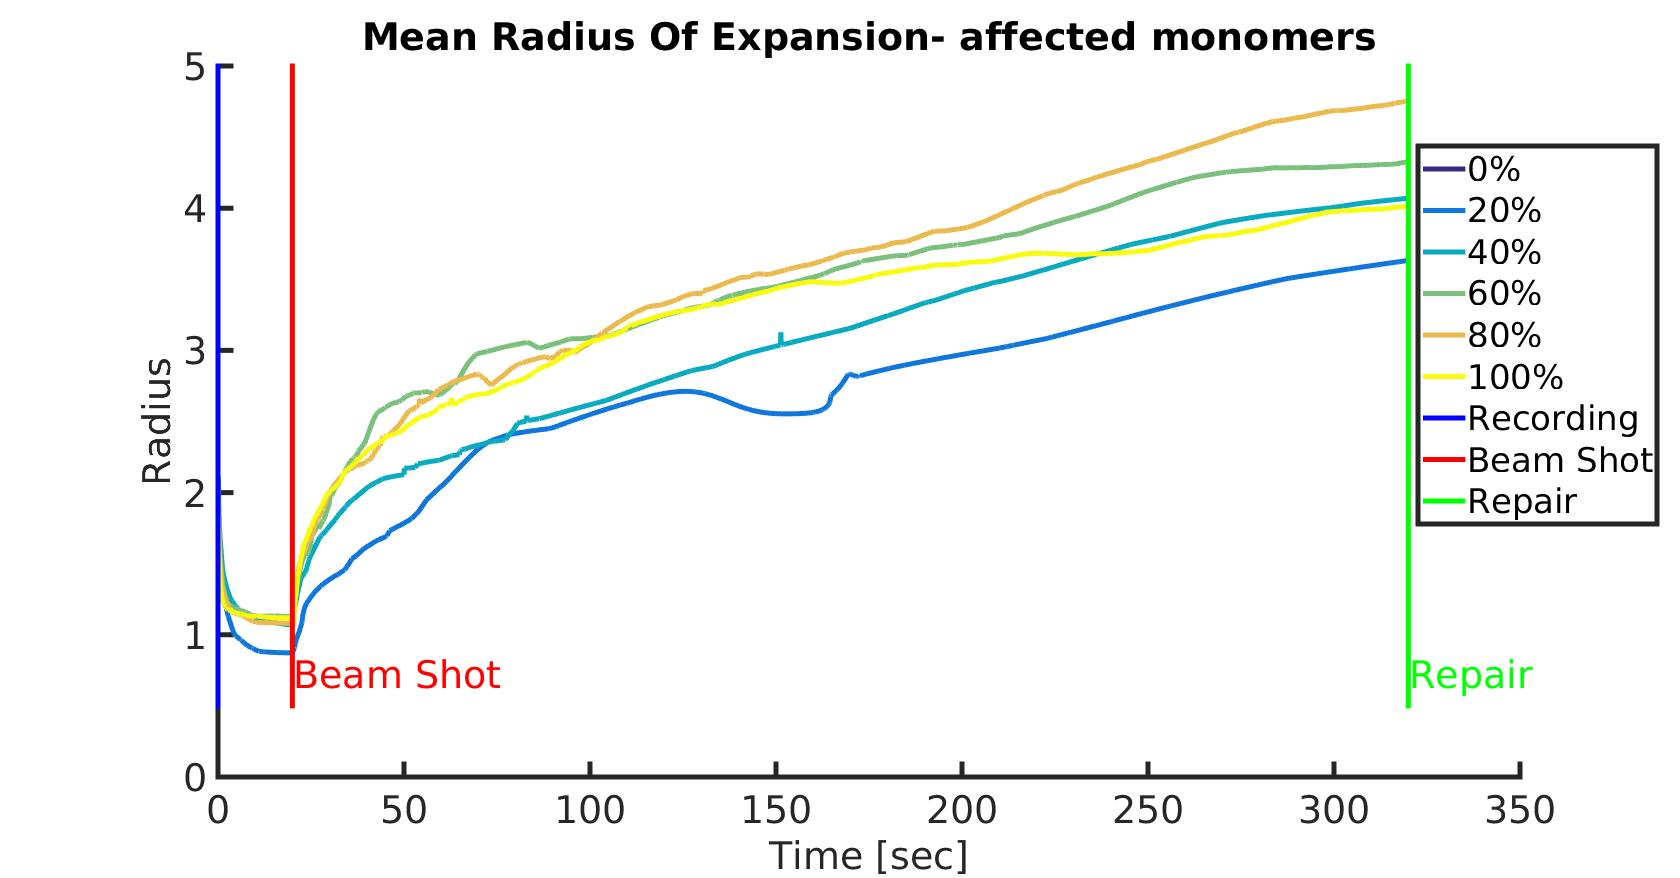
\includegraphics[width=0.5\linewidth, height=0.3\textheight]{Images/expandAffected/BreakAffectedCrosslinks/meanRadiusOfExpansionAffected}
	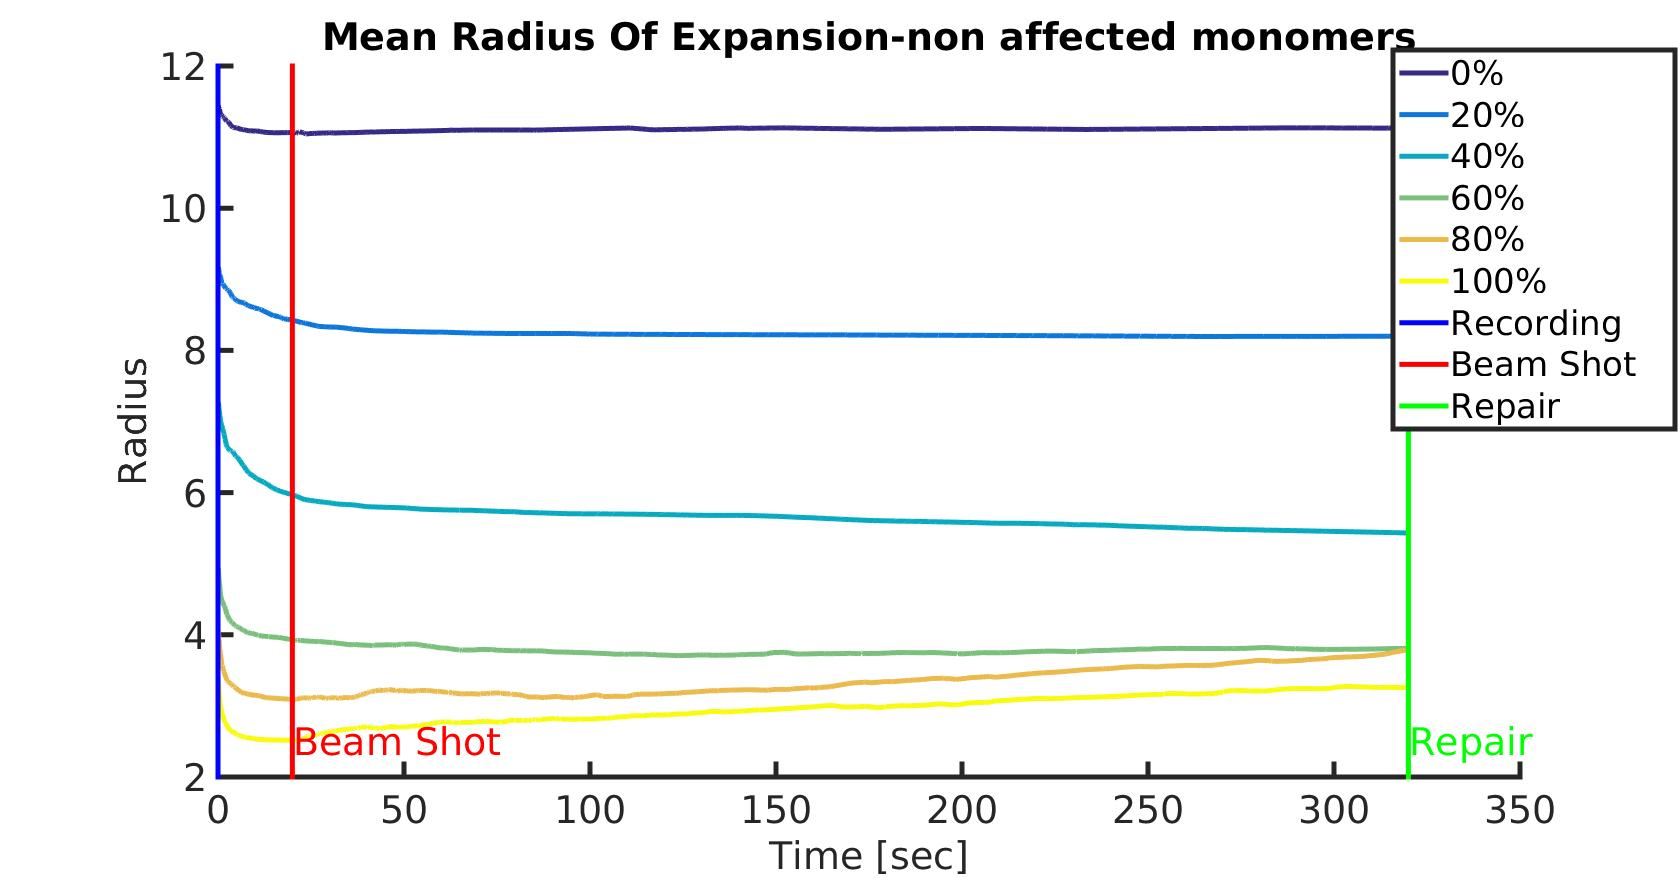
\includegraphics[width=0.5\linewidth, height=0.3\textheight]{Images/expandAffected/BreakAffectedCrosslinks/meanRadiusOfExpansionNonAffected}
	\caption{\tiny{\textbf{The radius of expansion for the affected (left) and non-affected (right) for a varying degree of connectivity. The cross-links to and from the damaged monomers are broken after UVC. As can be seen the affected monomer radius of expansion is increasing throughout the simulation, whereas the non- affected monomers remain static.  The polymer includes 500 monomers.The ROi is determined according to the damaged monomers.}}}
	\label{fig:meanRadiusOfExpansionAffectedBrokenCrosslinks}
	\end{figure}
	
	Examining the number and percentage of monomers in the ROI we have:
	
	\begin{figure}
	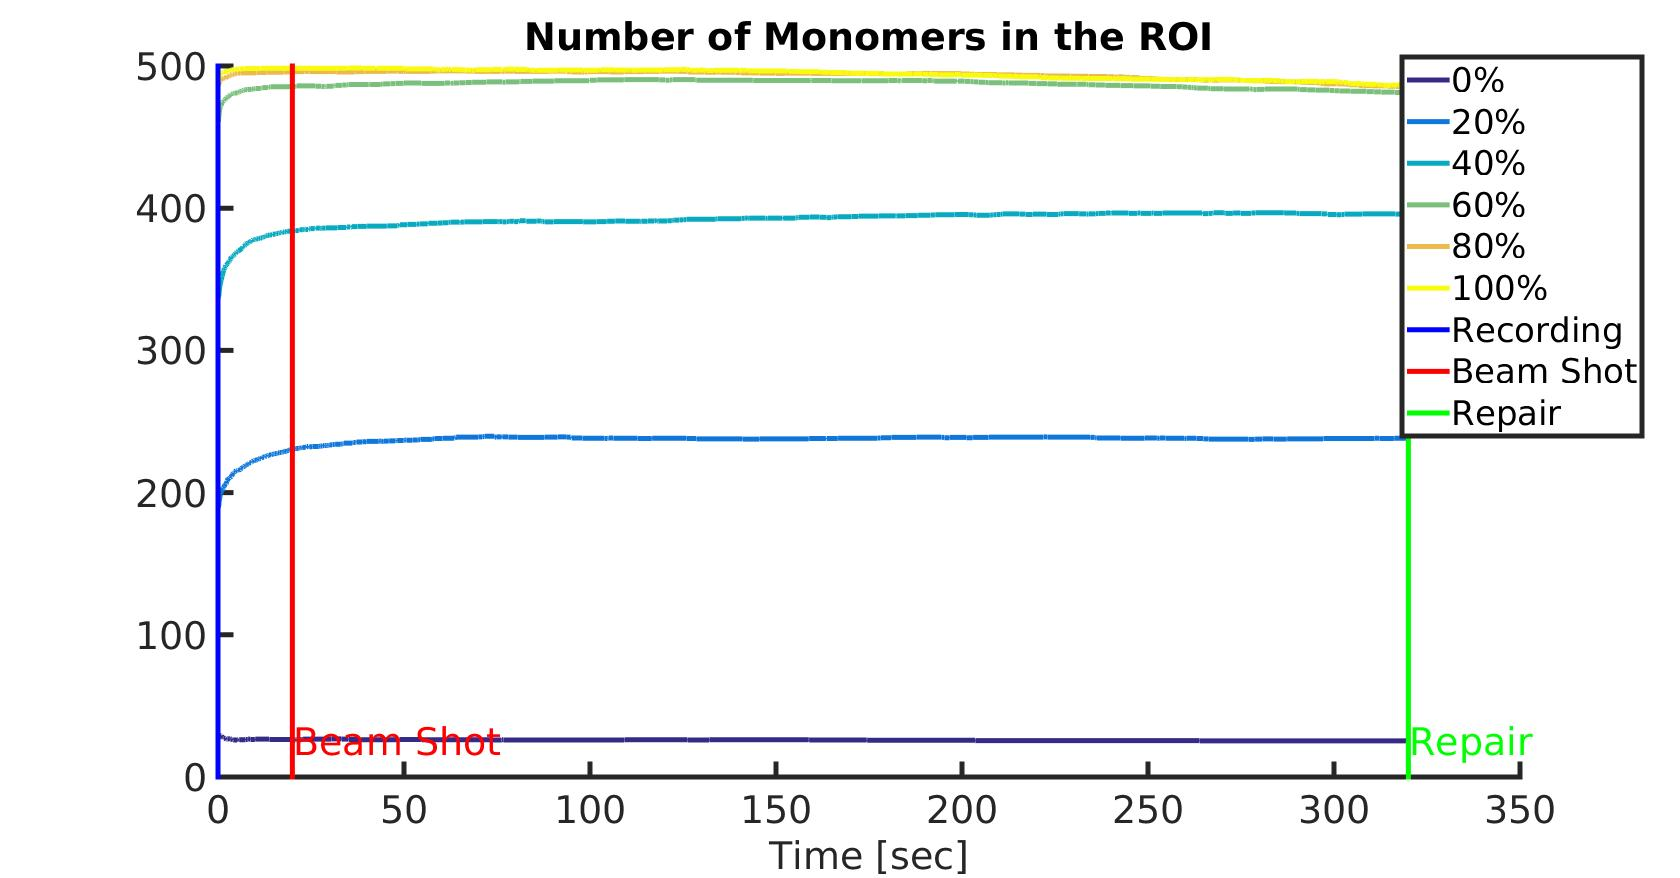
\includegraphics[width=0.5\linewidth, height=0.3\textheight]{Images/expandAffected/BreakAffectedCrosslinks/meanNumMonomersInROI}
	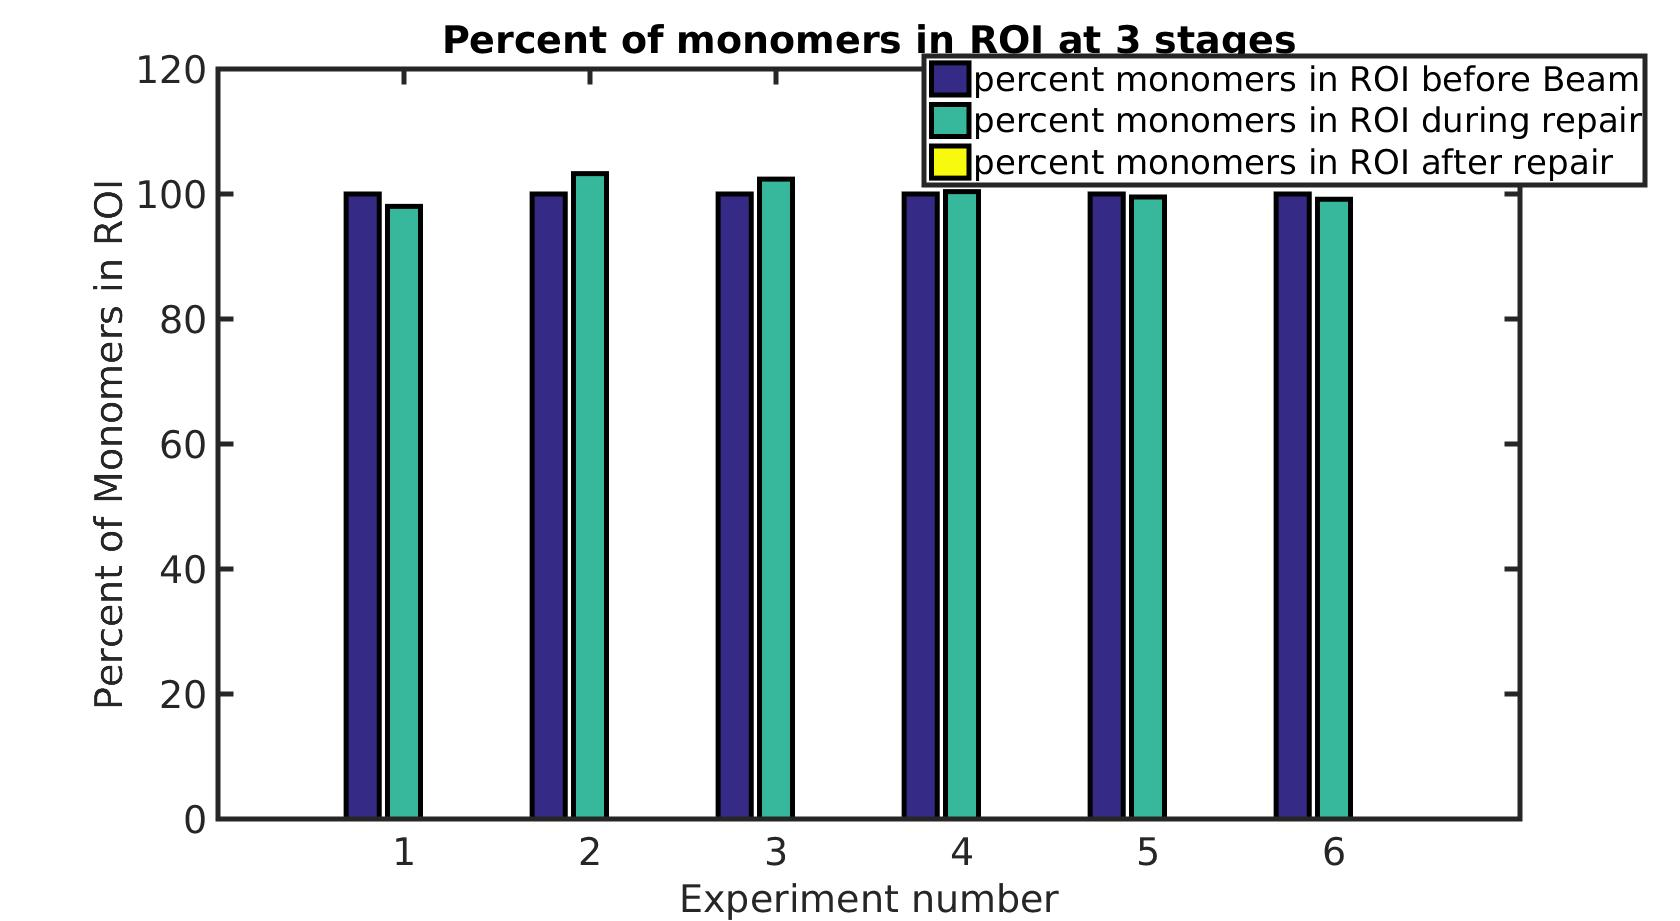
\includegraphics[width=0.5\linewidth, height=0.3\textheight]{Images/expandAffected/BreakAffectedCrosslinks/percentMonomersInROI}
	\caption{\tiny{\textbf{Number of monomers in ROI (left) and percentag (right) before and after UVC beam. No steps simulated past the repair phase. As can be seen, although the radius of the damaged monomers is increasing steadily, the number if monomers in the ROI remain roughly constant post UVC. In term of percentages, there seems to be no change.The polymer includes 500 monomers.The ROI is determined according to the damaged monomers.}}}
	\label{fig:meanNumMonomersInROI}
	\end{figure}
		
	
	\subsubsection{Keep all cross-links}
      \textbf{Experiment 1}
      
	   The radius of expansion of the damaged and non-damaged monomers was examined when no cross-links were broken post UVC. The ROI is determine according to the damaged monomers. The polymers contains 500 monomers. 
		     		     
		\begin{figure}[H]
		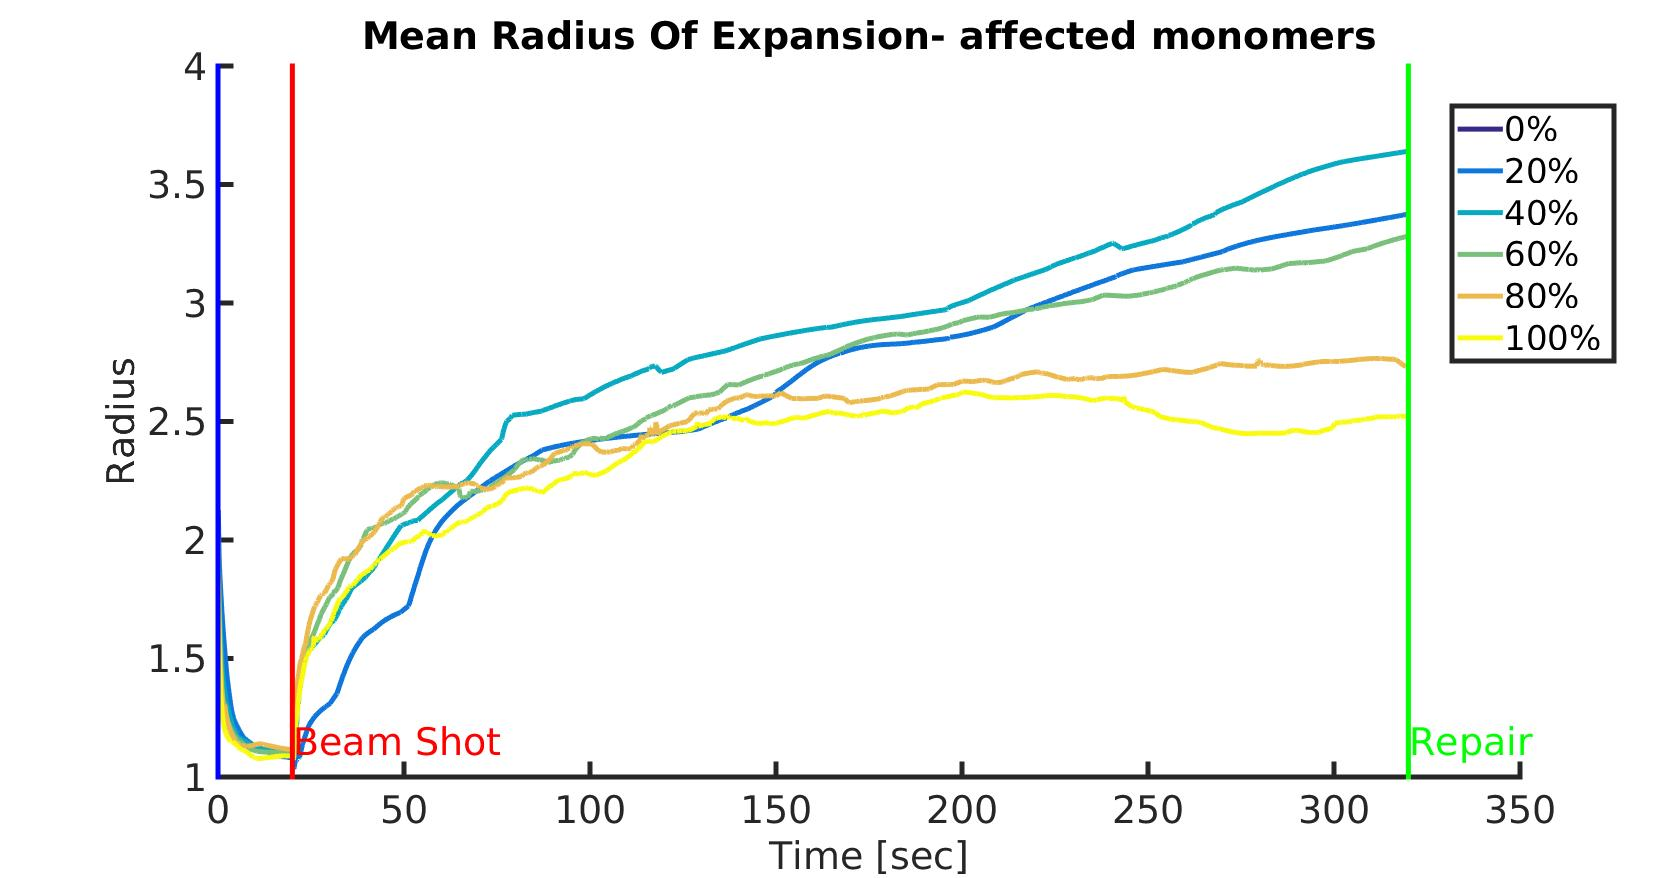
\includegraphics[width=0.5\linewidth, height=0.3\textheight]{Images/expandAffected/NoCrosslinksBroken/meanRadiusOfExpansionAffected}
		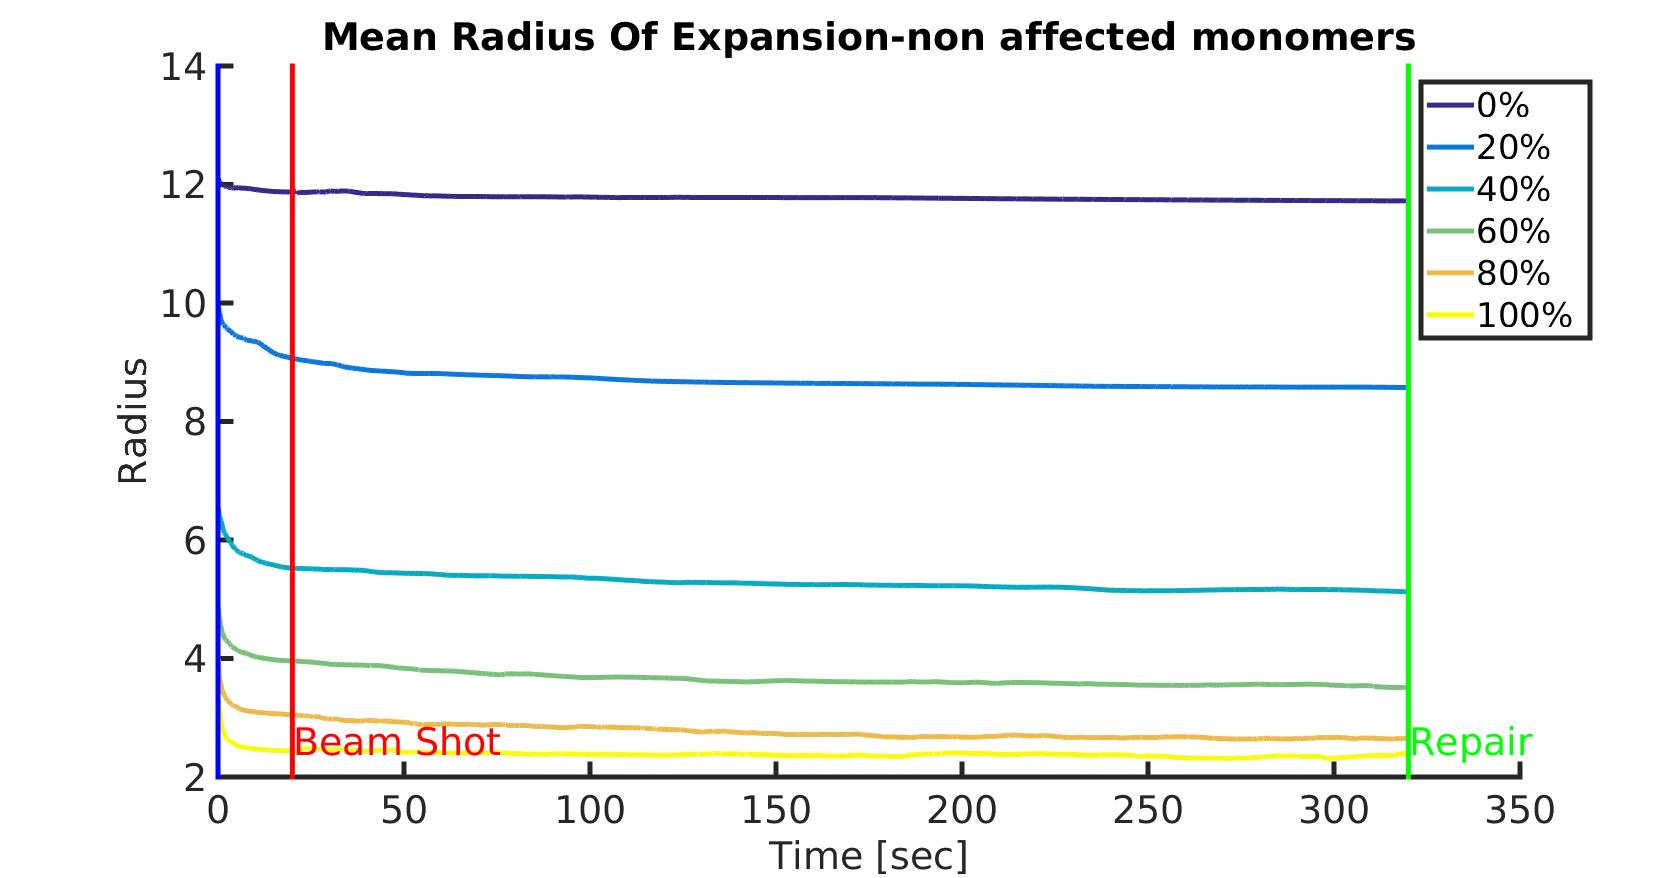
\includegraphics[width=0.5\linewidth, height=0.3\textheight]{Images/expandAffected/NoCrosslinksBroken/meanRadiusOfExpansionNonAffected}
		\caption{\tiny{\textbf{The radius of expansion for the damaged (left) and nono-damaged (right) monomers. Crosslinks are not removed after UVC. The polymer contains 500 monomers.}}}
		\label{fig:meanRadiusOfExpansionAffectedNoCrosslinksBroken}
		\end{figure}
			      
		 Examining the number and percentage of monomers in the ROI before and after UVC, we have:
		 		      
		\begin{figure}[H]
		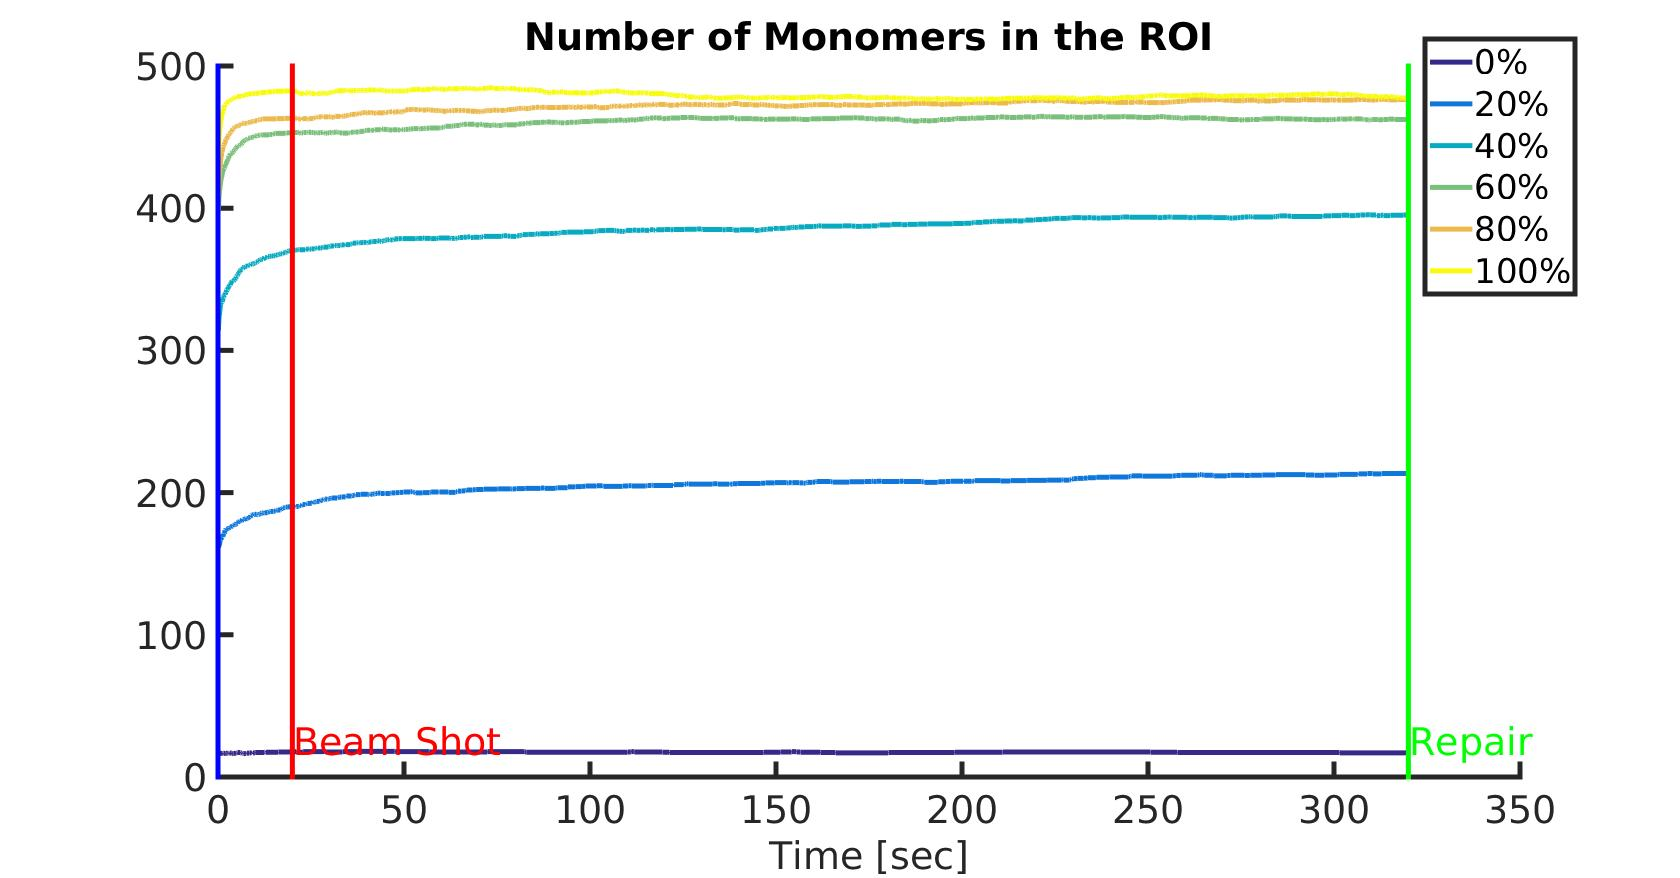
\includegraphics[width=0.5\linewidth, height=0.3\textheight]{Images/expandAffected/NoCrosslinksBroken/meanNumMonomersInROI}
		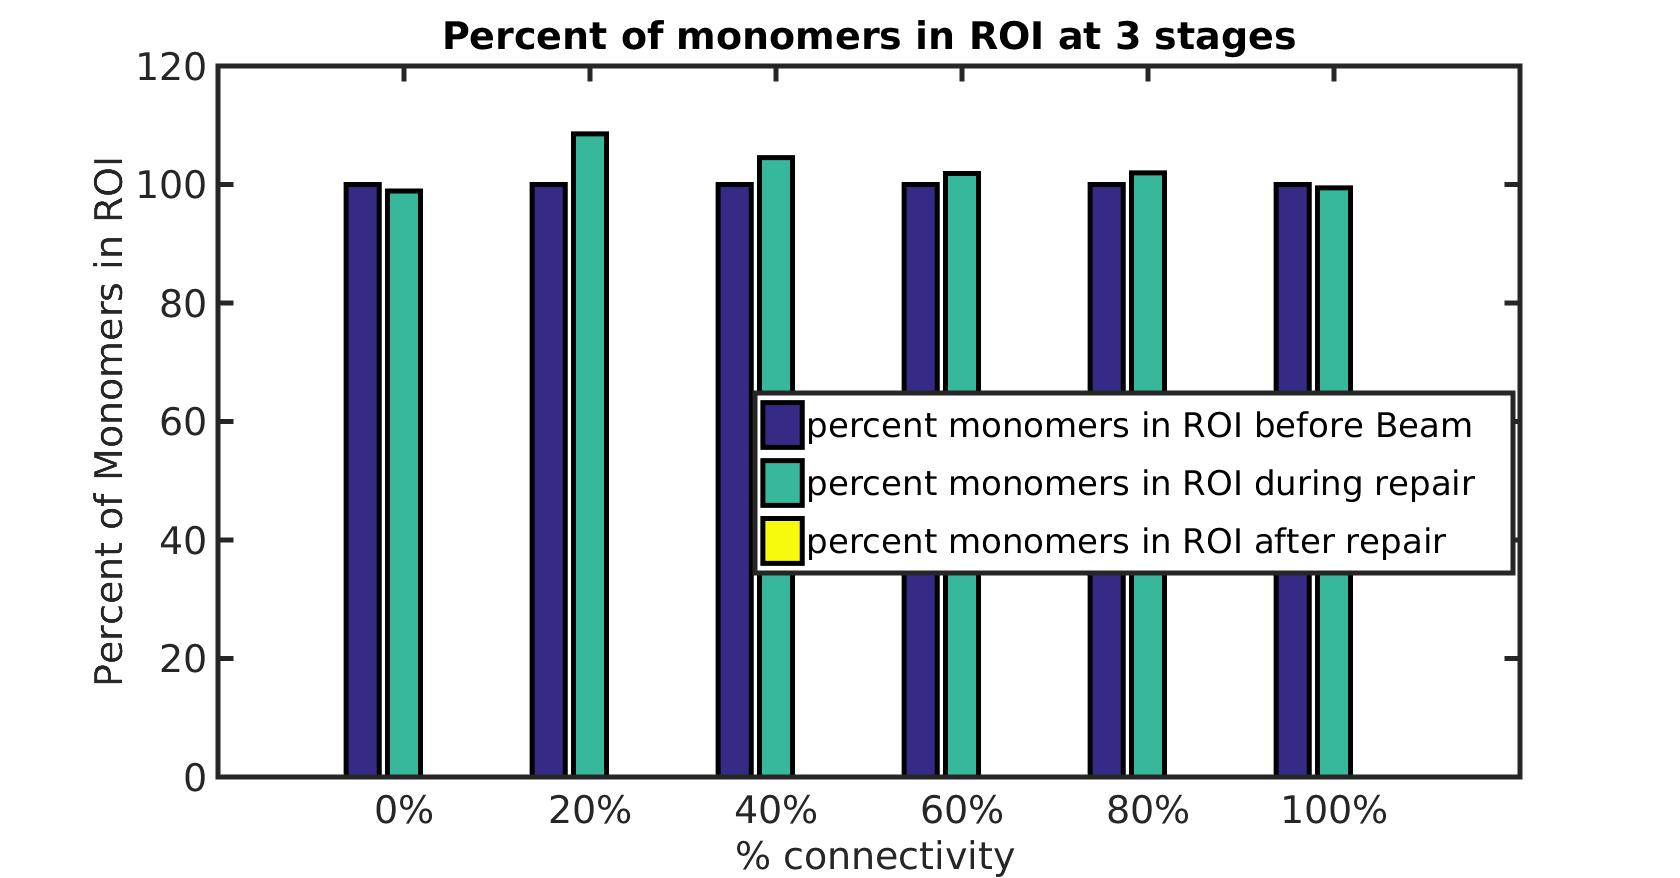
\includegraphics[width=0.5\linewidth, height=0.3\textheight]{Images/expandAffected/NoCrosslinksBroken/percentOfMonomersInROI}
		\caption{\tiny{\textbf{The number of monomers (left) and their percentages (right) in the ROI, when all crosslinks are kept after UVC. Although the radius of expansion for the affected monomers is increasing, the number of monomers in the ROI remains relatively constant. In terms of the percentages of monomers in the ROi, there seems to be no major changes. Values presented are the mean of 5 simulation with a polymer of 500 monomers for each connectivity percentage.}}}
		\label{fig:meanNumMonomersInROINoCrosslinkBroken}
		\end{figure}
		
				
	     \textbf{Experiment 2}
		     
	     We examine the radius of expansion for a more refined percentage of connectivity. When this experiment was conducted we did not yet program the ROI to be defined by the affected or non affected monomers after repair time. Therefore, the graphs of the number of monomers in the ROi and their percentages is missing. 
		     	     
	 	\begin{figure}[H]
	     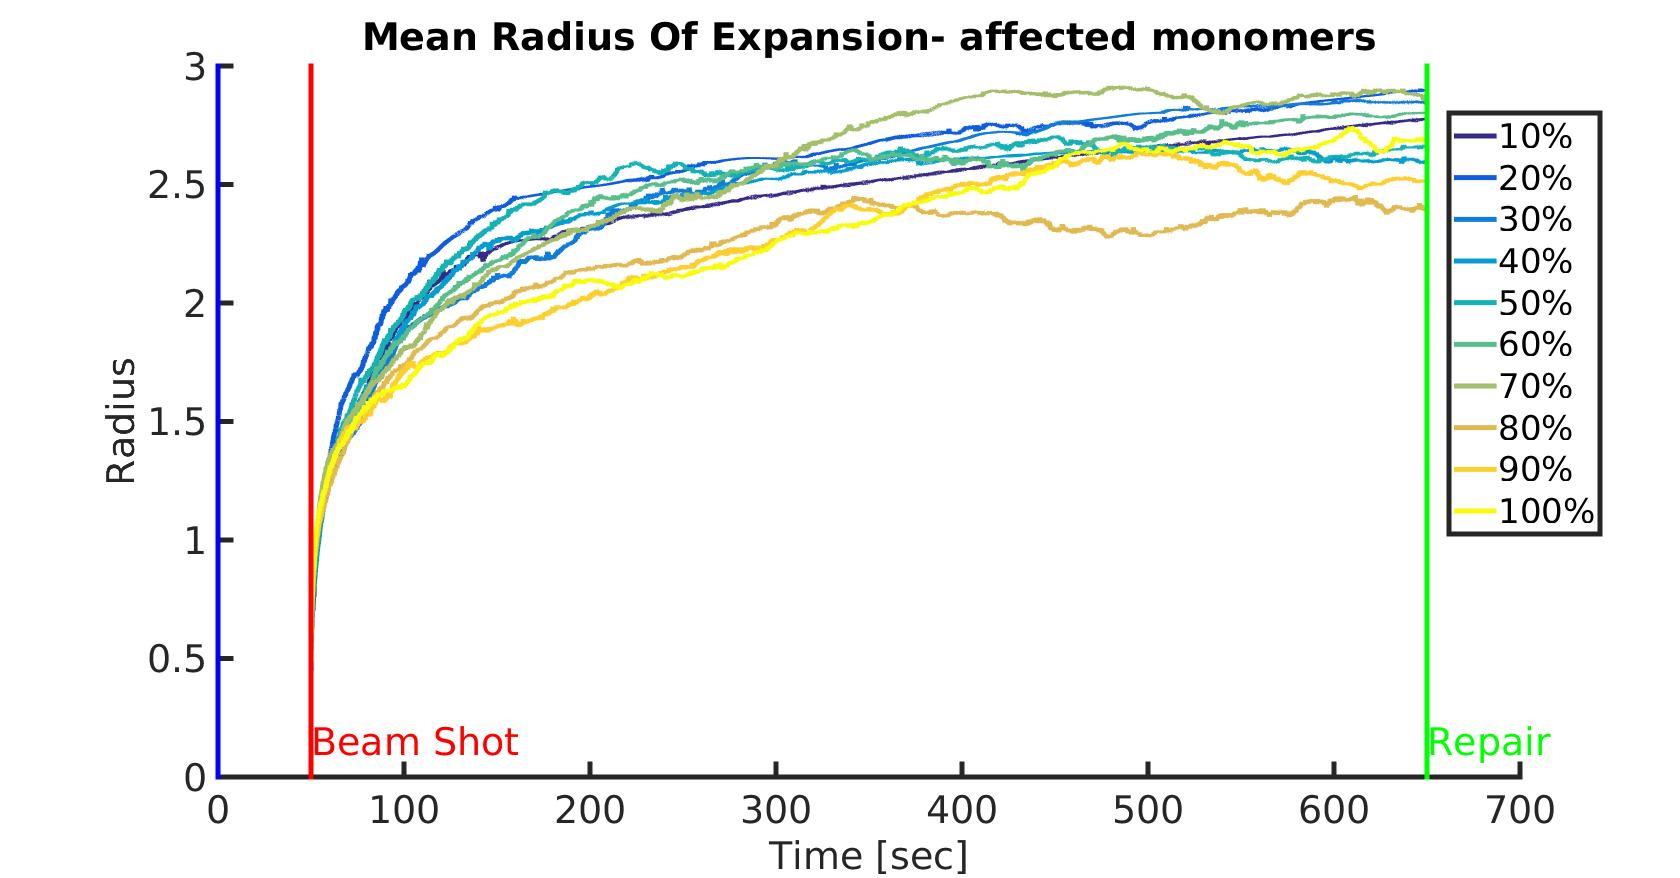
\includegraphics[width=0.5\linewidth,height=0.3\textheight]{RadiusOfExpansion500BeadsAffectedLennardJonesCrosslinked}
	     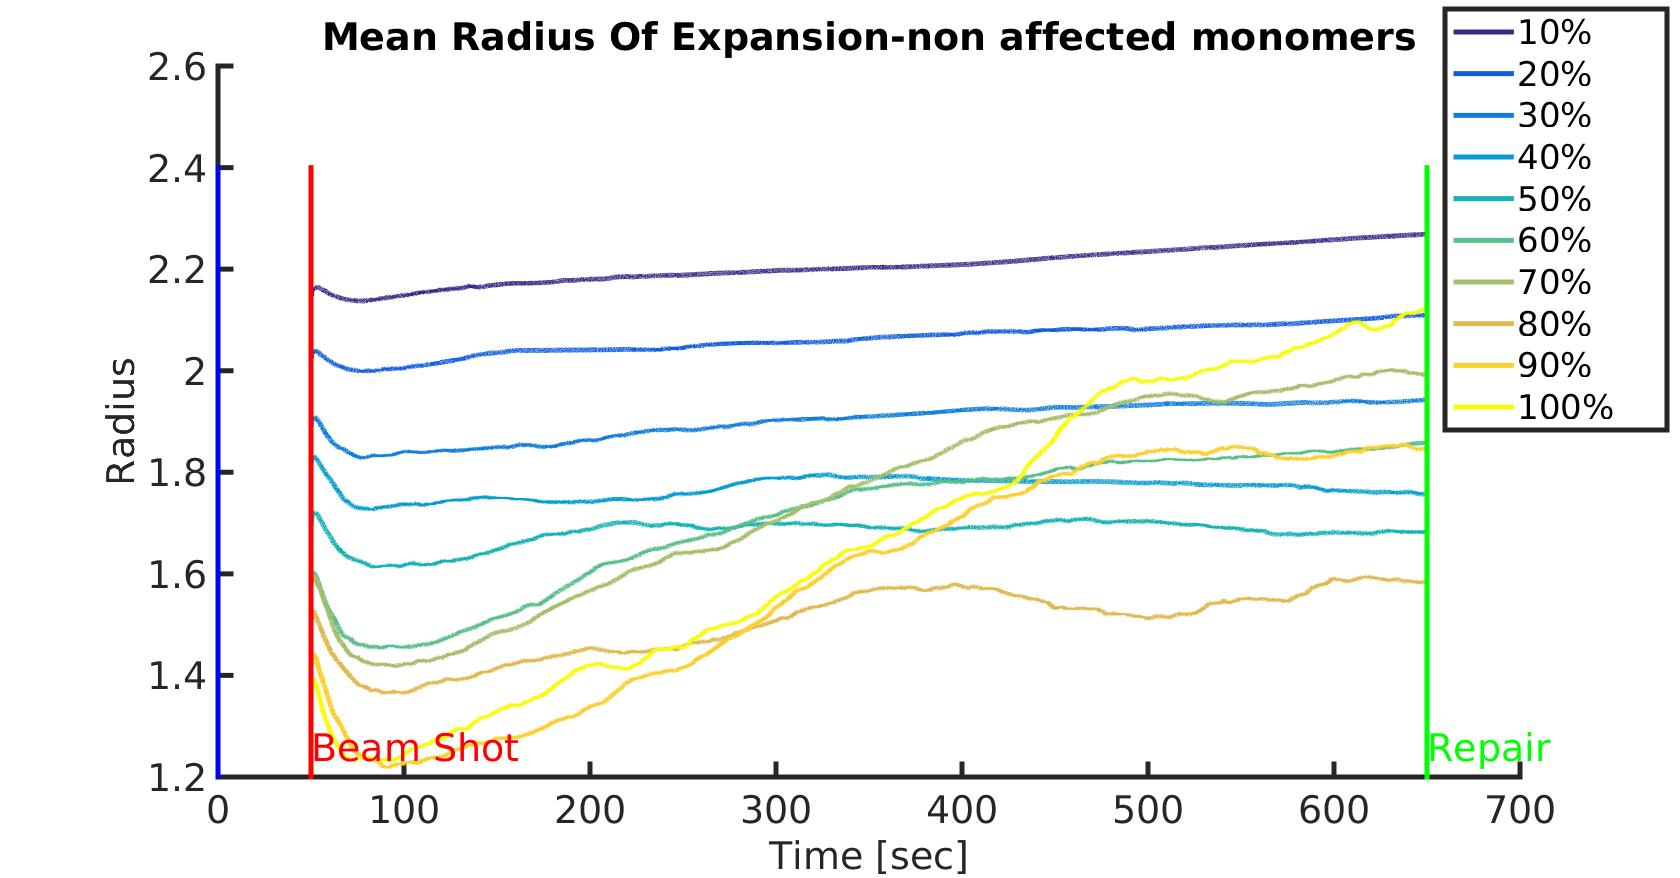
\includegraphics[width=0.5\linewidth,height=0.3\textheight]{RadiusOfExpansion500BeadsNonAffectedLennardJonesCrosslinked}
	      \caption{\tiny{\textbf{Radius of expansion for the affected (left) and non-affected (right) monomers, when the polymer is cross-linked by varying percentages. Expansion of the affected monomers is not stopped and goes beyond the non-affected expansion radius. (500 monomers with Lennard-Jones force)}}}
		     \label{fig:RadiusOfExpansion500BeadsAffectedLennardJonesCrosslinked}
    	\end{figure}
		      		
     	As can be seen from Figure \ref{fig:RadiusOfExpansion500BeadsAffectedLennardJonesCrosslinked} even with cross-links, and the given parameter set, expansion of the damaged monomers is not stopped. 
	  	Because the region of interest to measure density in is determined post-prior to the expansion, this will pose a problem, since the ROI will include also the non-damaged monomers, which do not seem to expand much in low percentages of cross-linking.
		      		
	  	This brings us to believe that high level of connectivity is needed, where both the affected and non-affected radius of expansion increases (see, for example, the curves for 80-100\% connectivity in Figure \ref{fig:RadiusOfExpansion500BeadsAffectedLennardJonesCrosslinked}). In that scenario, the ROI, which is determined at the end of the beam steps will more likely represent the expanded area seen in experiments, in which we see 20\% loss of DNA. 
		      		
	  	Two monomers of a cross-linked polymer are more likely to be found in the center. In a cross-linked polymer, after we shut-down diffusion, there is a convergence toward the center because all cross-links are pulling towards one another. This creates the situation in which the damaged monomers do not have to expand much to pass the cross-linked layer of the non-damaged monomers. 
	
	\subsection{Assign bending to non-damaged monomers}
		
		The result of the previous subsection brought us to believe that the expansion should not occur in the damaged monomers but rather in the non-damaged ones i.e. The 20\% lose in DNA density should be attributed to the non-damaged monomers. The damaged DNA remains within the repair zone, whereas non-damaged DNA is pushed aside by the repair mechanism. According to this scenario, the simulation now captures the following process:
		\begin{enumerate}
			\itemsep0em
			\item cross-linked polymer is being shot by UVC;
			\item cross-links to and from the damaged monomers are released;
			\item repair mechanism pushes the non-damaged monomers out of the way, this causes bending elasticity for the non-damaged monomers.
		\end{enumerate}
		
		An alternative to step 3 is to assign bending elasticity to undamaged monomers in the UVC beam. The two alternative will be examined next.
		
	\subsubsection{Break damaged monomers' cross-links}
     After UVC we remove all cross-links to and from any damaged monomer. No Lennard-Jones potential is used. The ROI is determined according to the expansion of the damaged monomers, whereas we assign bending elasticity to the non-damaged monomers. 
          
	\begin{figure}[H]
	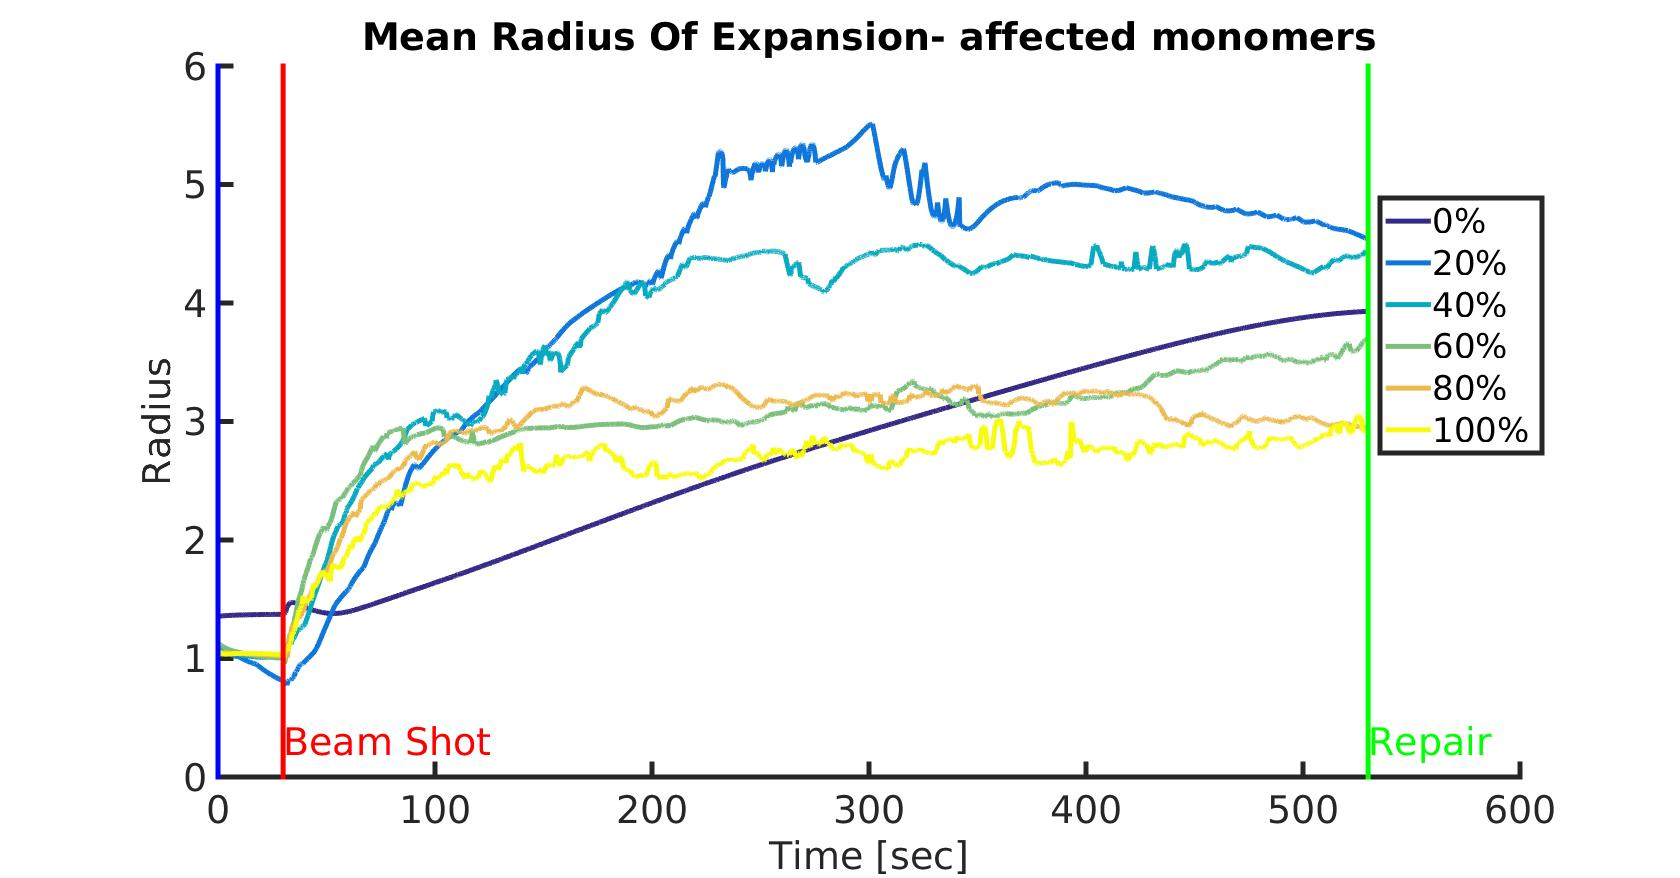
\includegraphics[width=0.5\linewidth, height=0.3\textheight]{Images/expandNonDamaged/BreakAffectedCrosslinks/04/MeanRadiusOfExpansionAffected}
    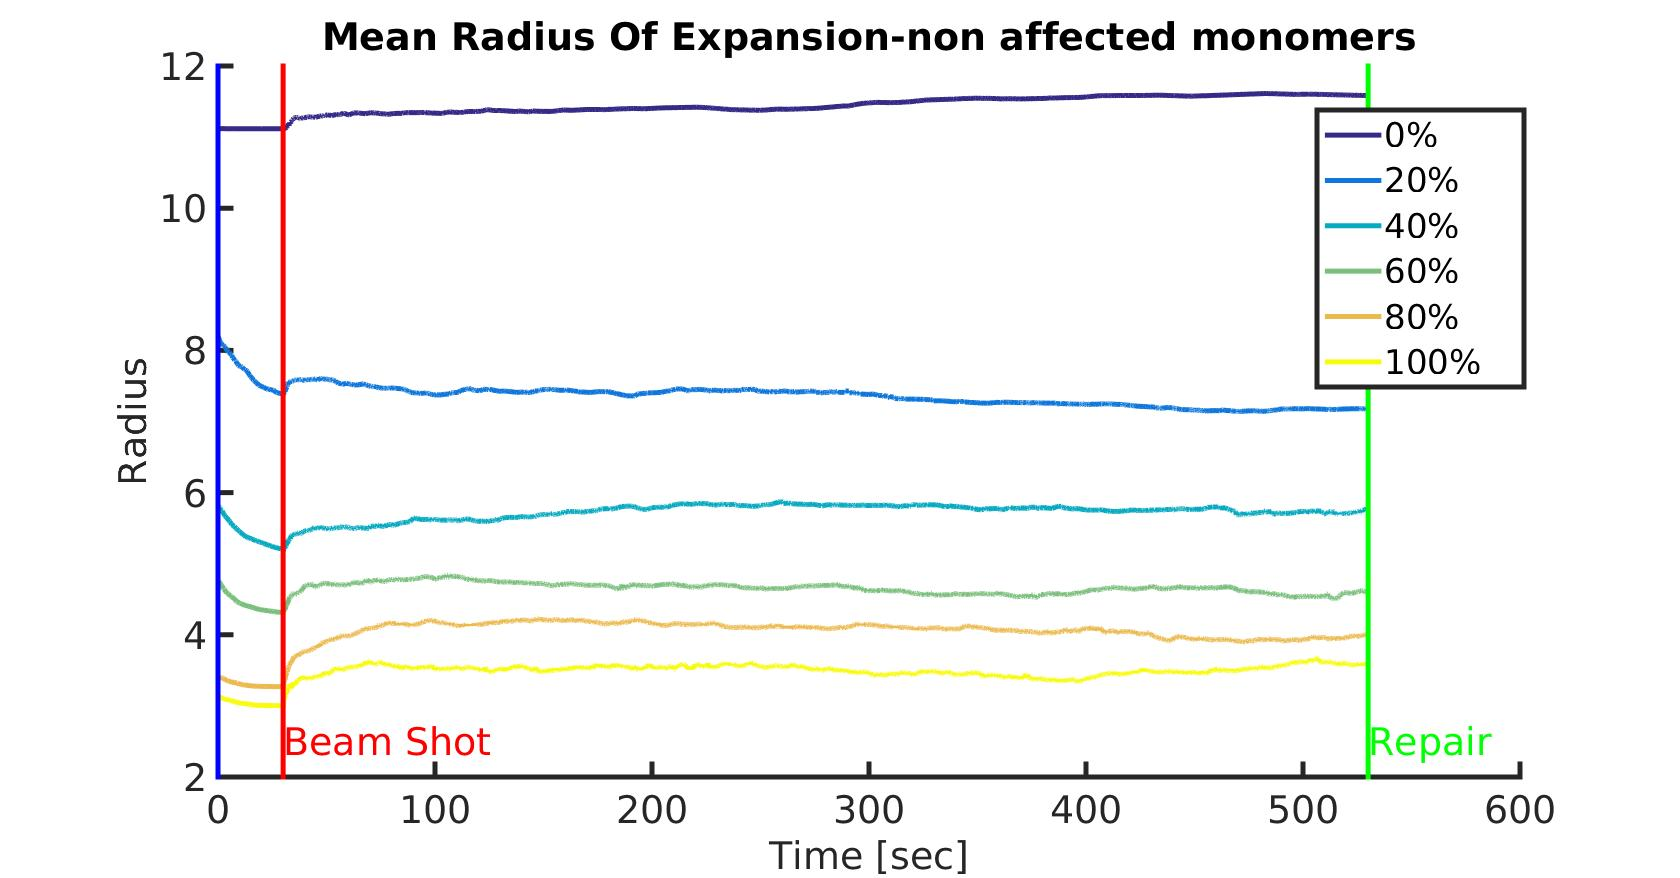
\includegraphics[width=0.5\linewidth, height=0.3\textheight]{Images/expandNonDamaged/BreakAffectedCrosslinks/04/MeanRadiusOfExpansionNonAffected}
	\caption{\tiny{\textbf{Mean Radius of expansion of the damaged (left) and non-damaged (right) monomers. As can be seen,  the radius of expansion for the affected monomers remains relatively small in comparison to the non-damaged in all experiments. (500 monomers, bending non-affected, no Lennard-Jones)}}}
	\label{fig:MeanRadiusOfExpansionAffected}
	\end{figure}
	     
	In terms of the number and percentage of monomers lose from ROI, we have:
	\begin{figure}[H]
	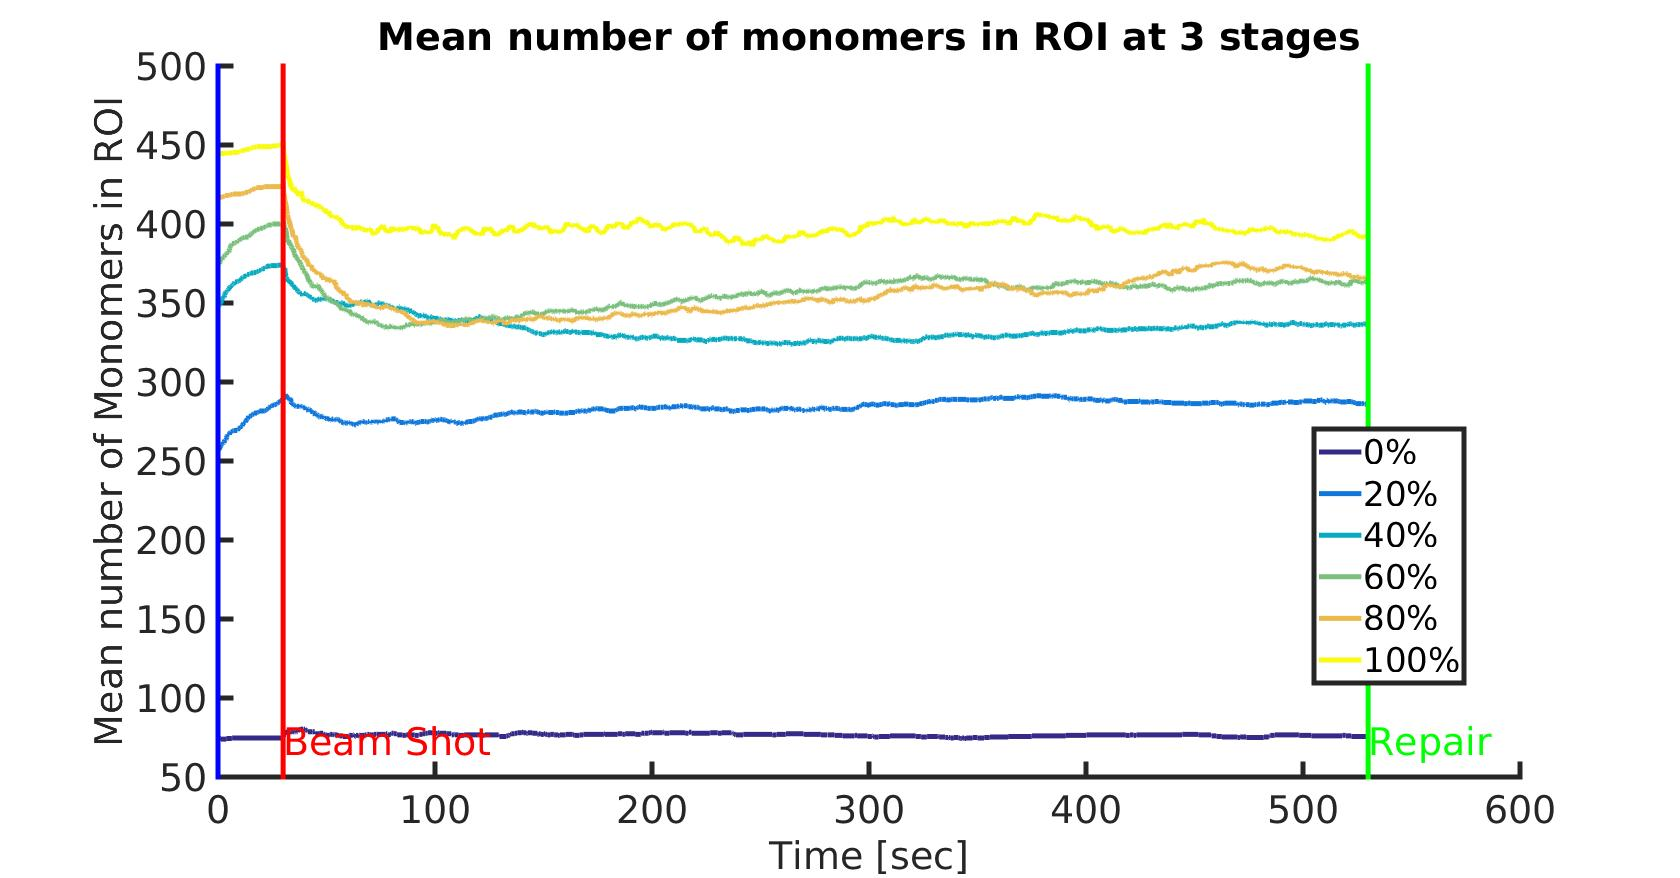
\includegraphics[width=0.5\linewidth, height=0.3\textheight]{Images/expandNonDamaged/BreakAffectedCrosslinks/04/MeanNumMonomersInROI}
	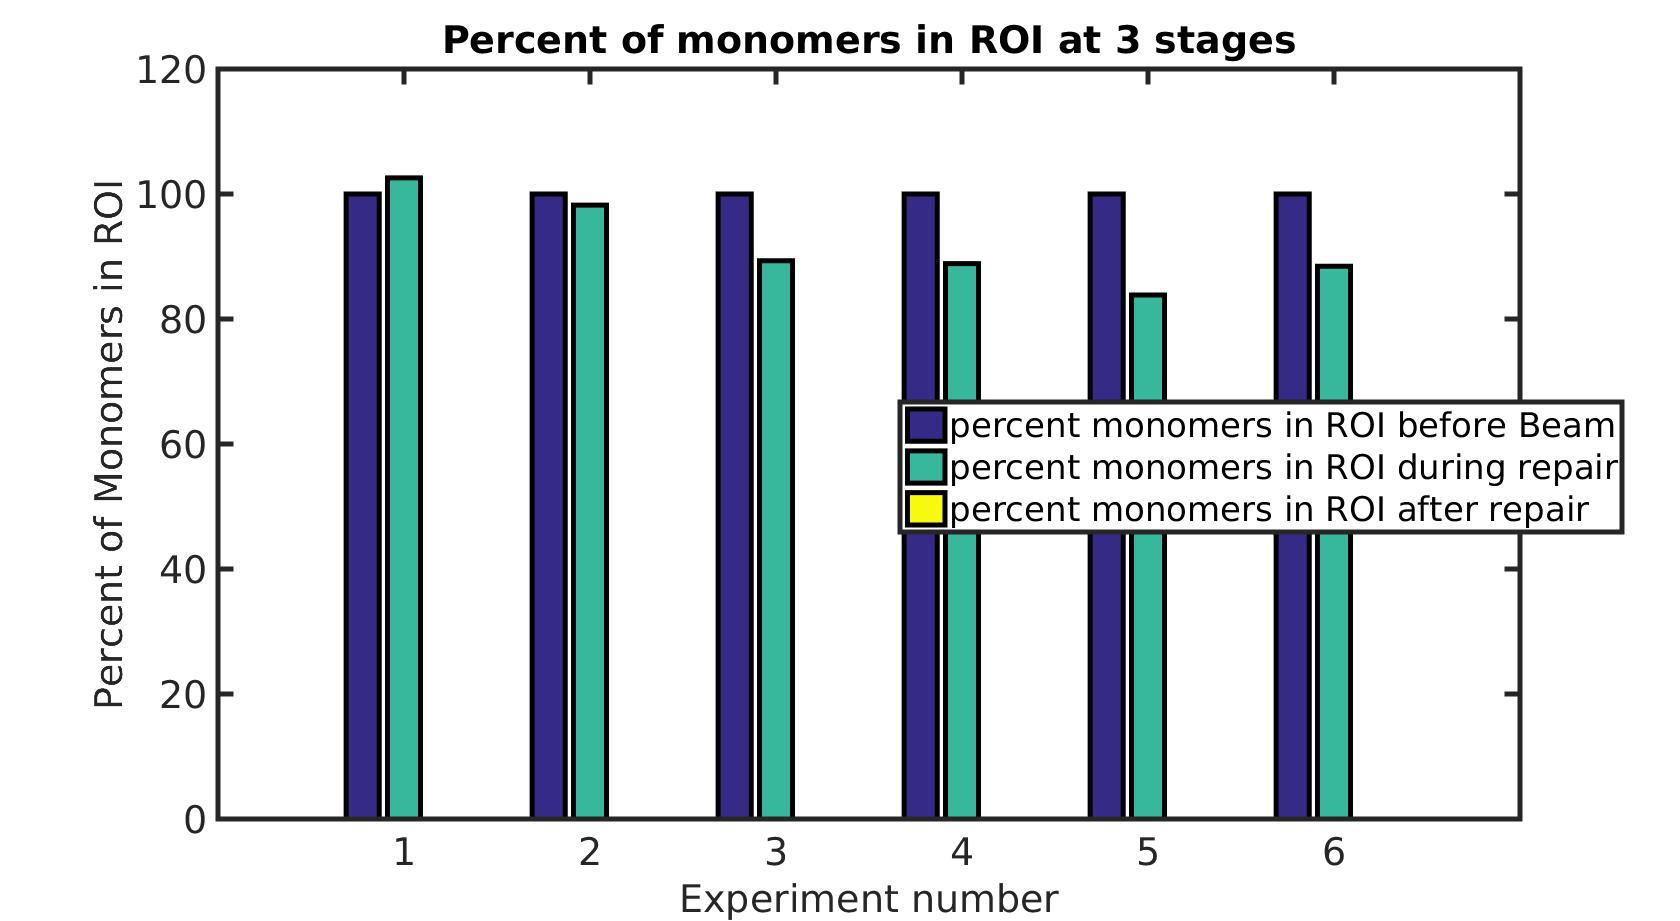
\includegraphics[width=0.5\linewidth, height=0.3\textheight]{Images/expandNonDamaged/BreakAffectedCrosslinks/04/percentOfMonomersInROI}
	\caption{\tiny{\textbf{The number of monomers in the ROI (left) with time and the overall percentage in comparison to the Recordign phase. As can be seen a loos of 20\% monomers from the ROI can be obtained with 80-100\% connectivity  (500 monomers, expanding non-affected, non Lennard-Jones)}}}
	\label{fig:MeanNumMonomersInROI}
	\end{figure}
	     For 80-100\% connectivity we can gain loss of 20\% monomers from the ROI. We now turn to explore more in-depth the parameters around 80\% connectivity. 
	     										
		\begin{figure}[H]
		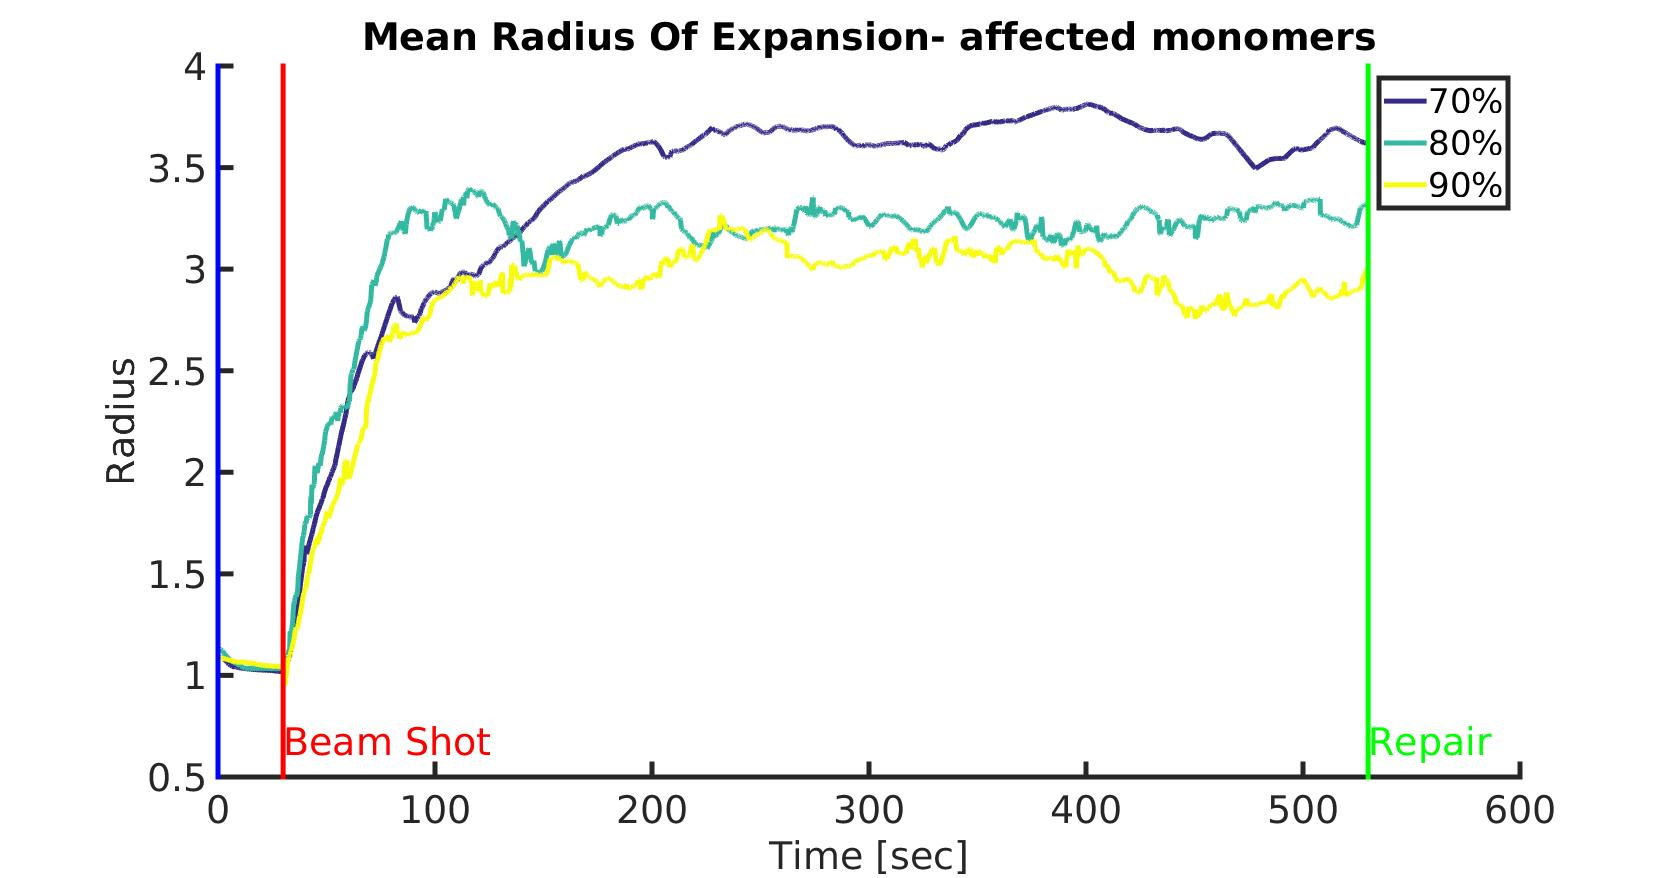
\includegraphics[width=0.5\linewidth, height=0.3\textheight]{Images/expandNonDamaged/BreakAffectedCrosslinks/05/meanRadiusOfExpansionAffected}
	    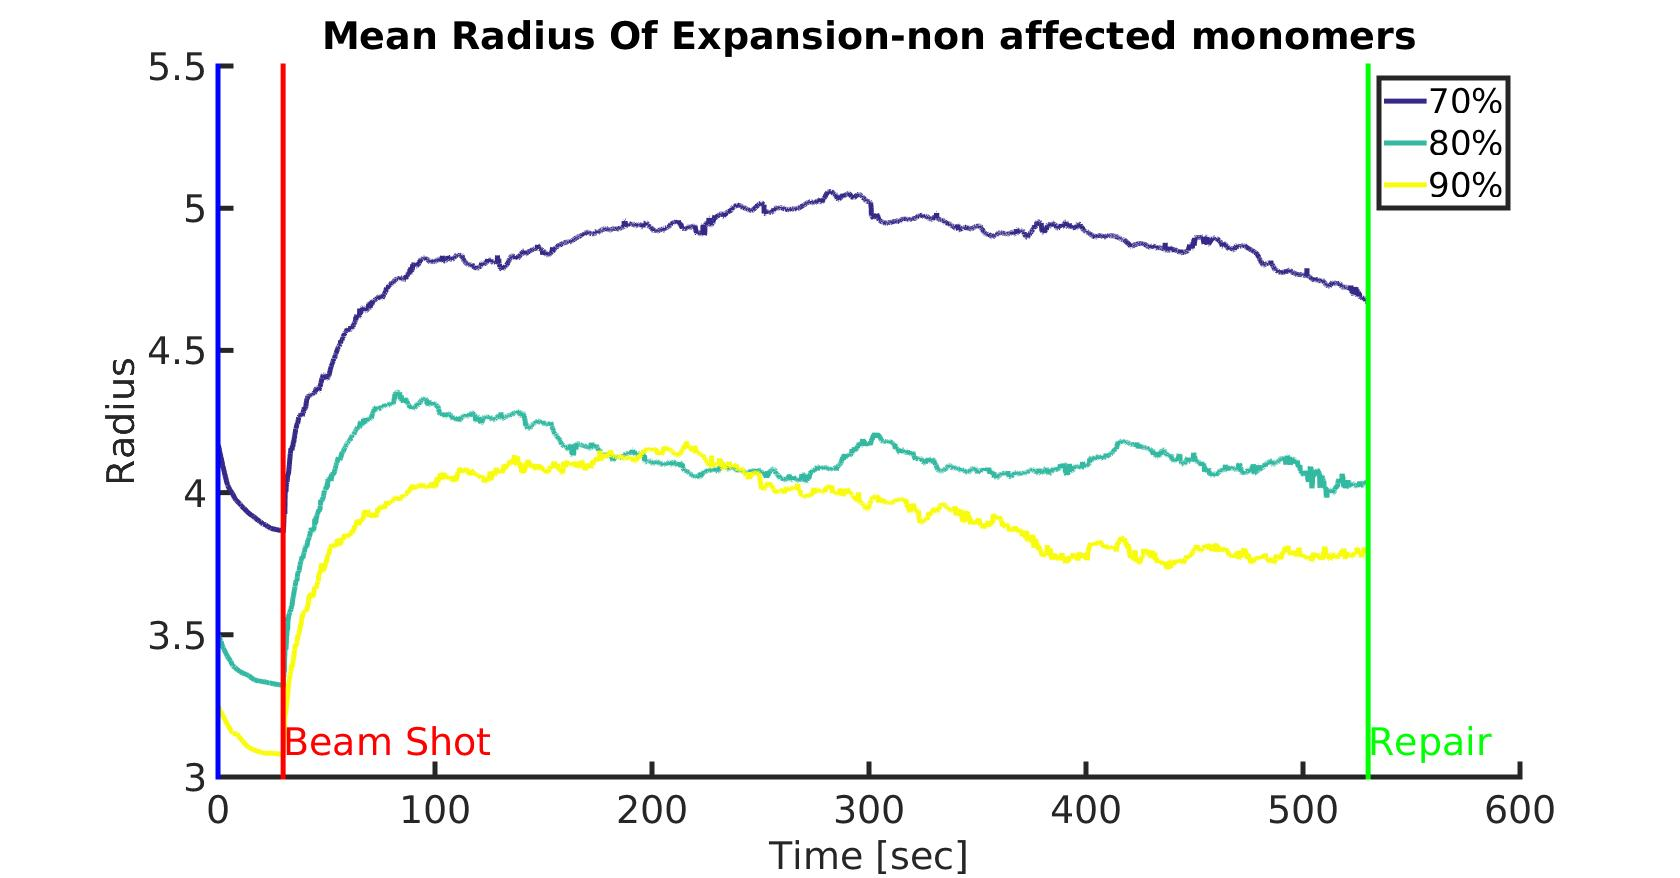
\includegraphics[width=0.5\linewidth,
		height=0.3\textheight]{Images/expandNonDamaged/BreakAffectedCrosslinks/05/meanRadiusOfExpansionNonAffected}
		\caption{}
		\label{fig:meanRadiusOfExpansionBendingNonAffectedBreakDamagedCrosslinks}
		\end{figure}
		
			
		\begin{figure}[H]
		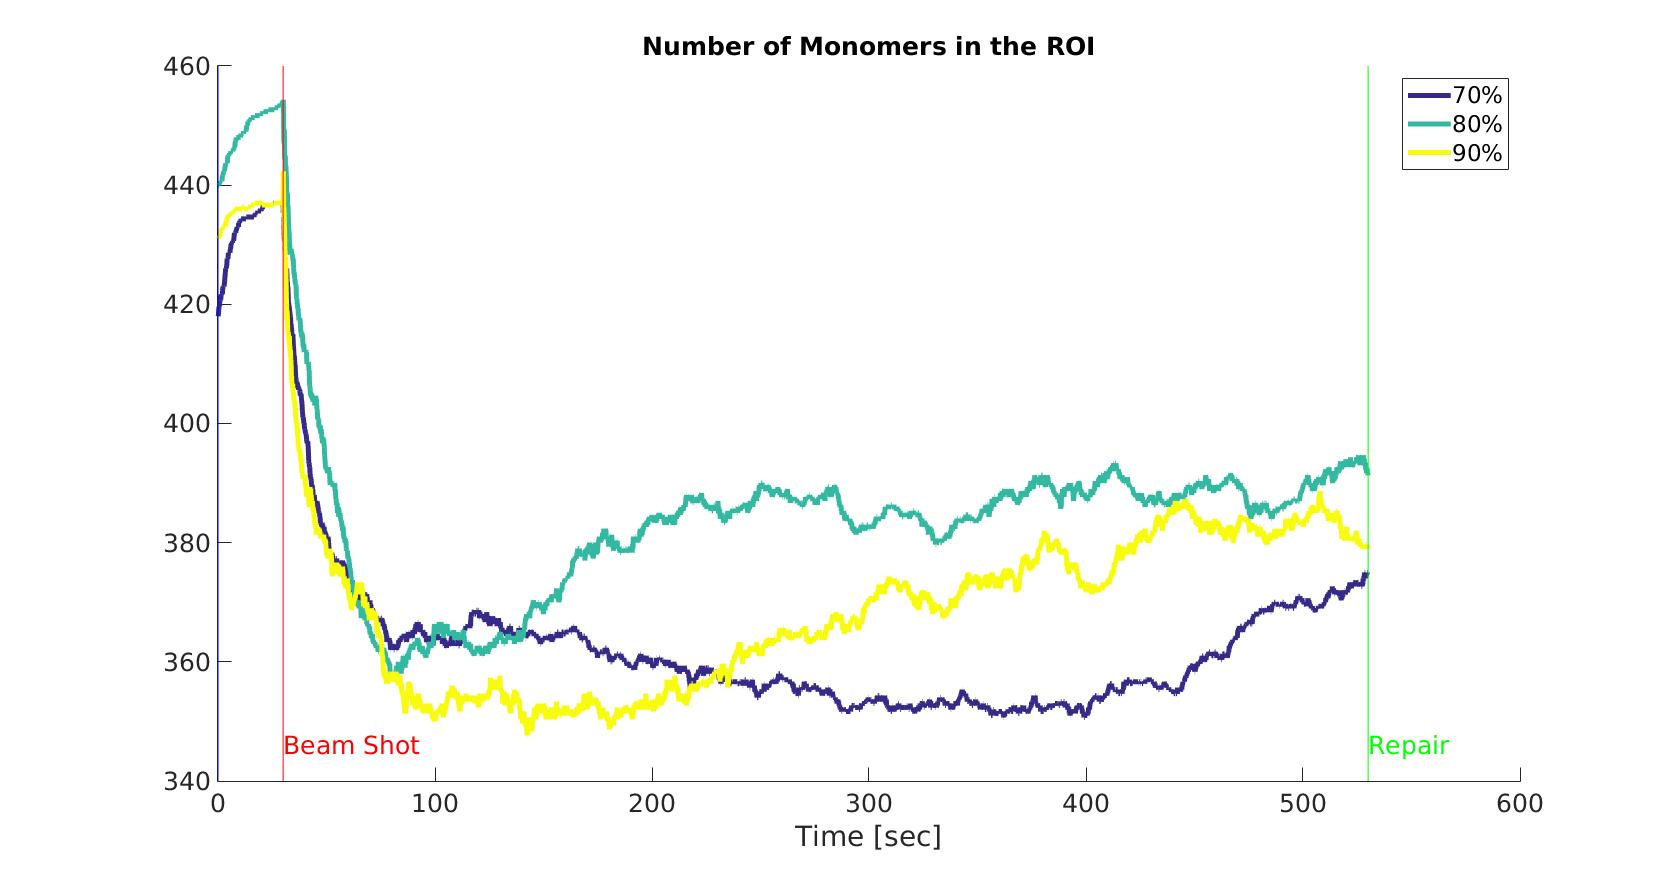
\includegraphics[width=0.5\linewidth, height=0.3\textheight]{Images/expandNonDamaged/BreakAffectedCrosslinks/05/meanNumMonomersInROI}
		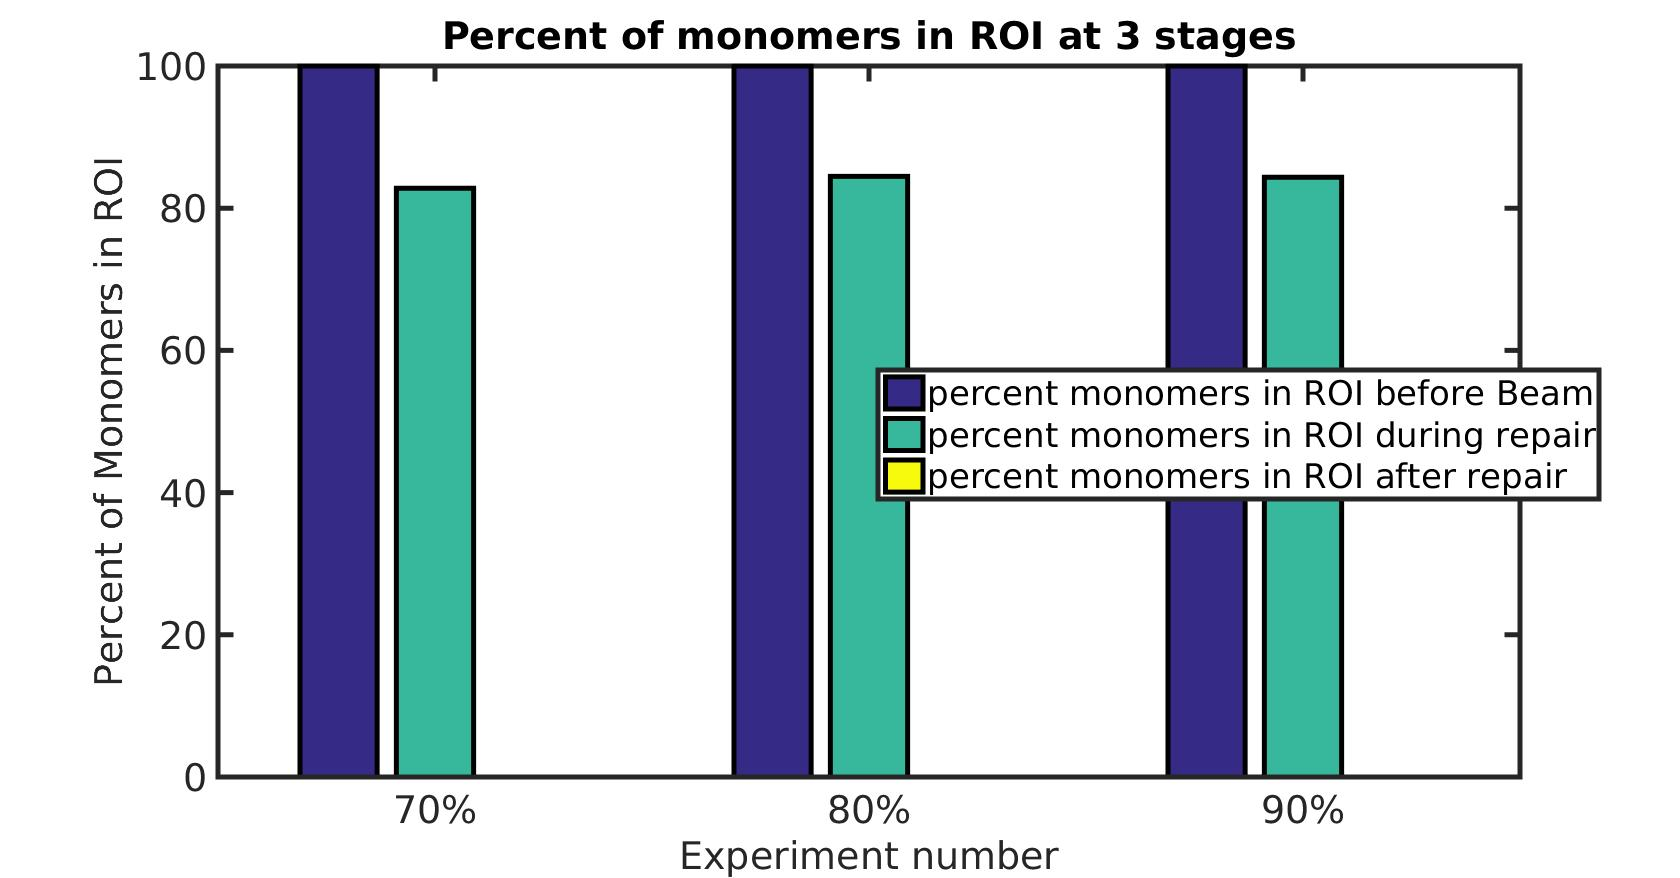
\includegraphics[width=0.5\linewidth, height=0.3\textheight]{Images/expandNonDamaged/BreakAffectedCrosslinks/05/percentageOfMonomersInROI}
		\caption{}		
		\label{fig:percentageOfMonomersInROI}
		\end{figure}
		
		
			
	\subsubsection{Keeping all cross-links after UVC}
		Keeping all cross-links, either	inside or outside the beam, while assigning bending only to non-damaged monomers we have:
		
	\begin{figure}[H]
	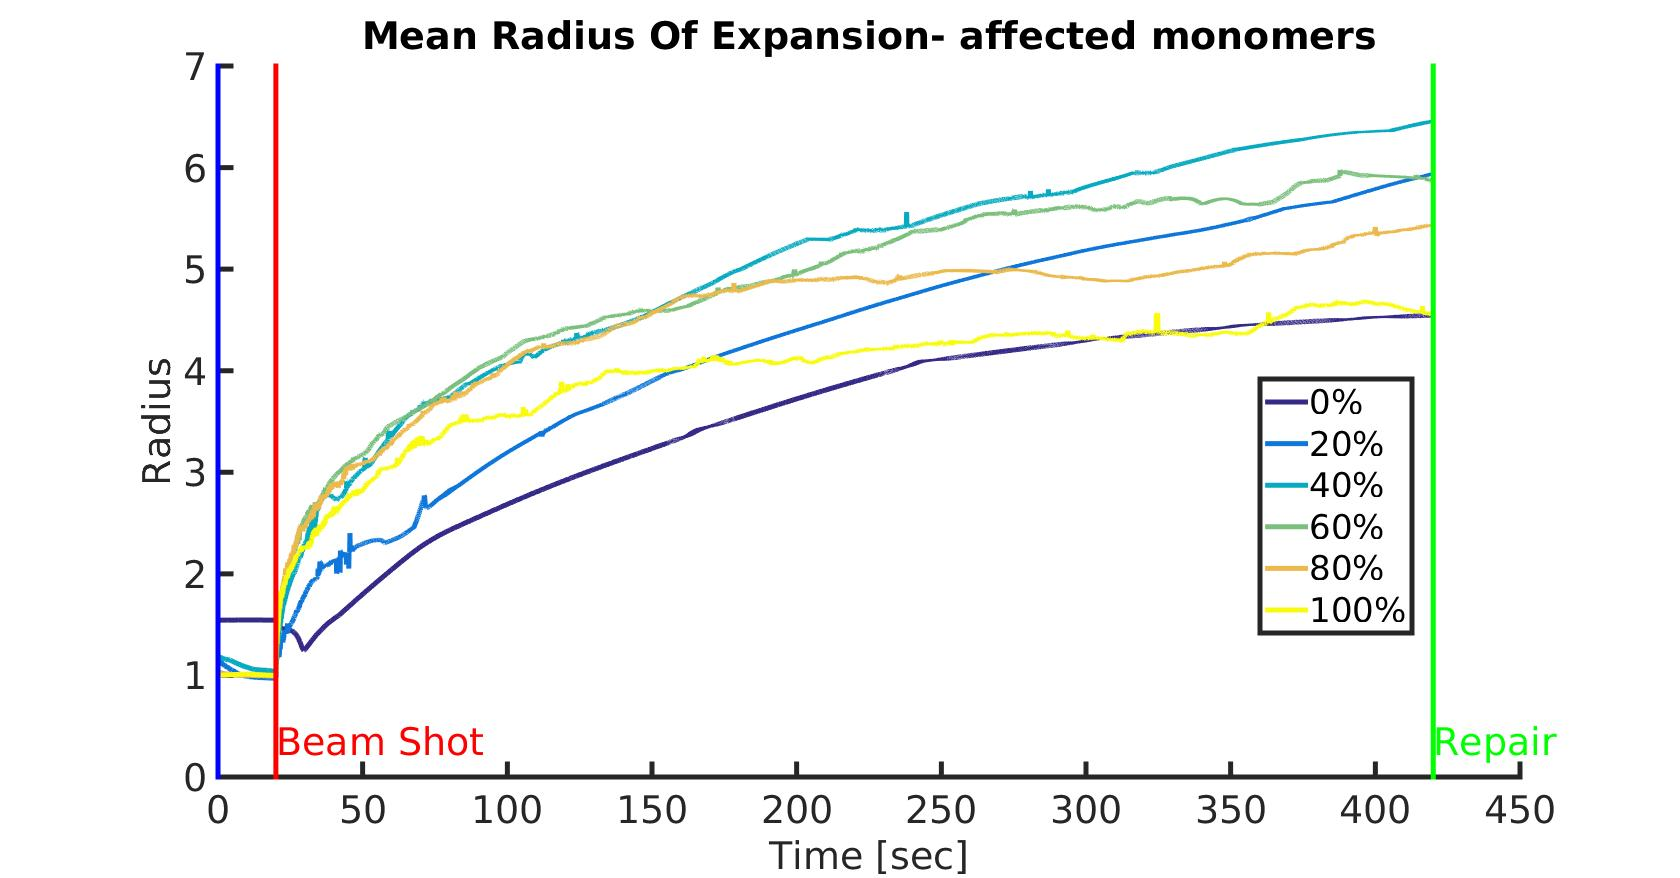
\includegraphics[width=0.5\linewidth]{Images/expandNonDamaged/NoCrosslinksBroken/meanRadiusOfExpansionAffected}
	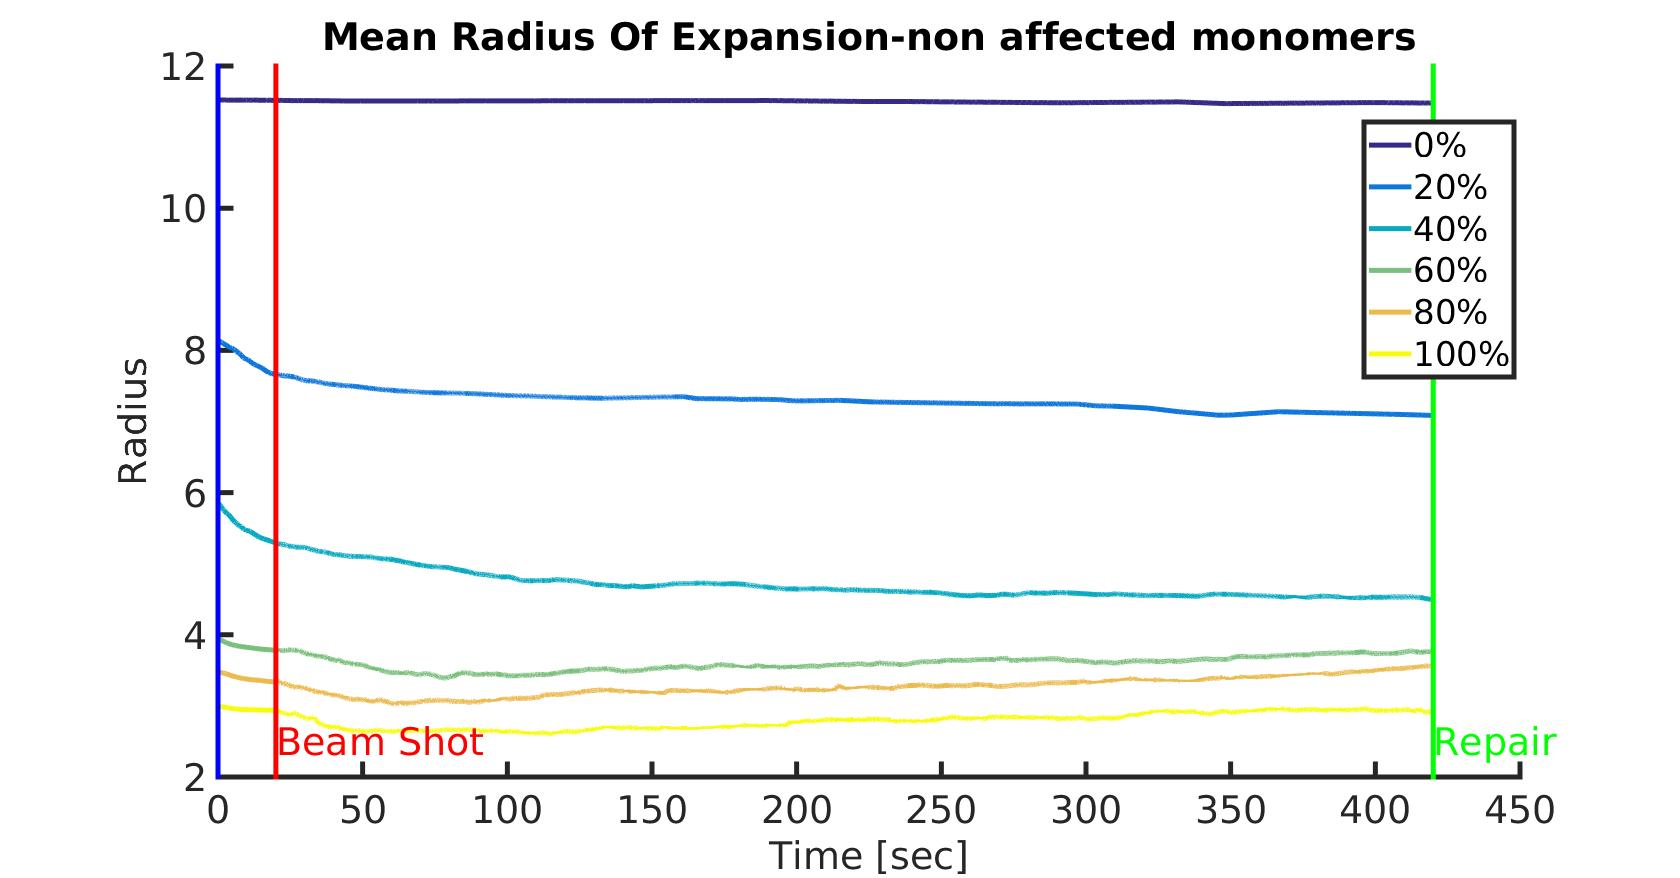
\includegraphics[width=0.5\linewidth]{Images/expandNonDamaged/NoCrosslinksBroken/meanRadiusOfExpansionNonAffected}
	\caption{\tiny{\textbf{Mean radius of expansion for the damaged (left) and undamaged (right) monomers. No cross-link is broken after UVC. The expansion of the damaged monomers is equivalent to that off the non-damaged.}}}
	\label{fig:meanRadiusOfExpansionBendingNonAffecteNoBrokenCrosslinks}
	\end{figure}
	In terms of the loss of monomers in the ROI, we have:
	
	\begin{figure}[H]
	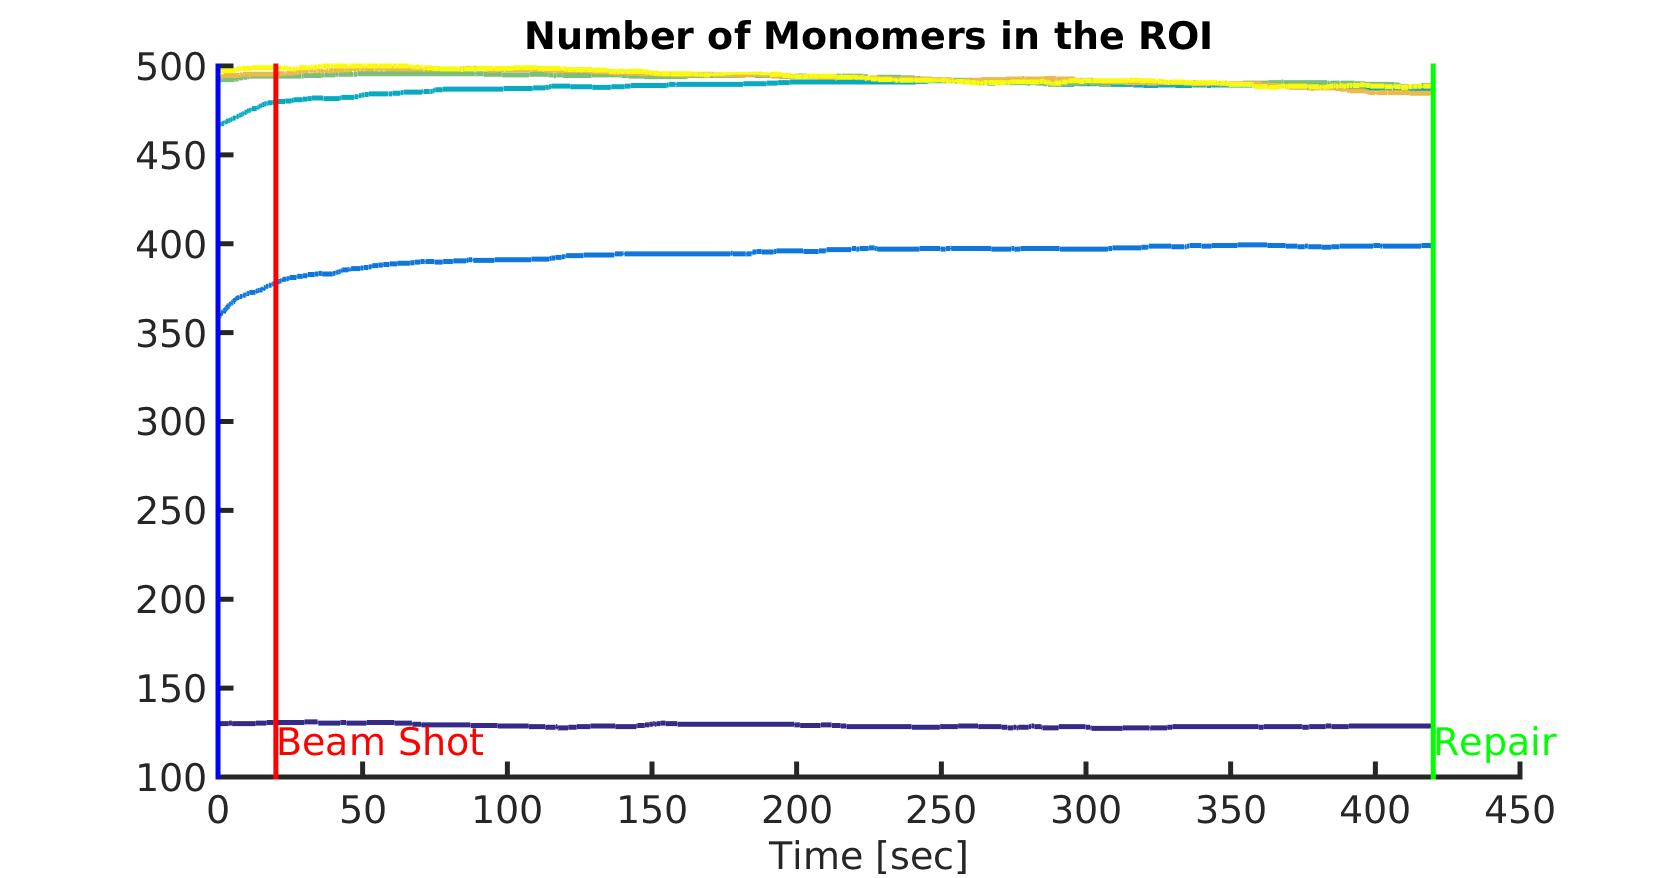
\includegraphics[width=0.5\linewidth, height=0.3\textheight]{Images/expandNonDamaged/NoCrosslinksBroken/meanNumMonomersInROI}
	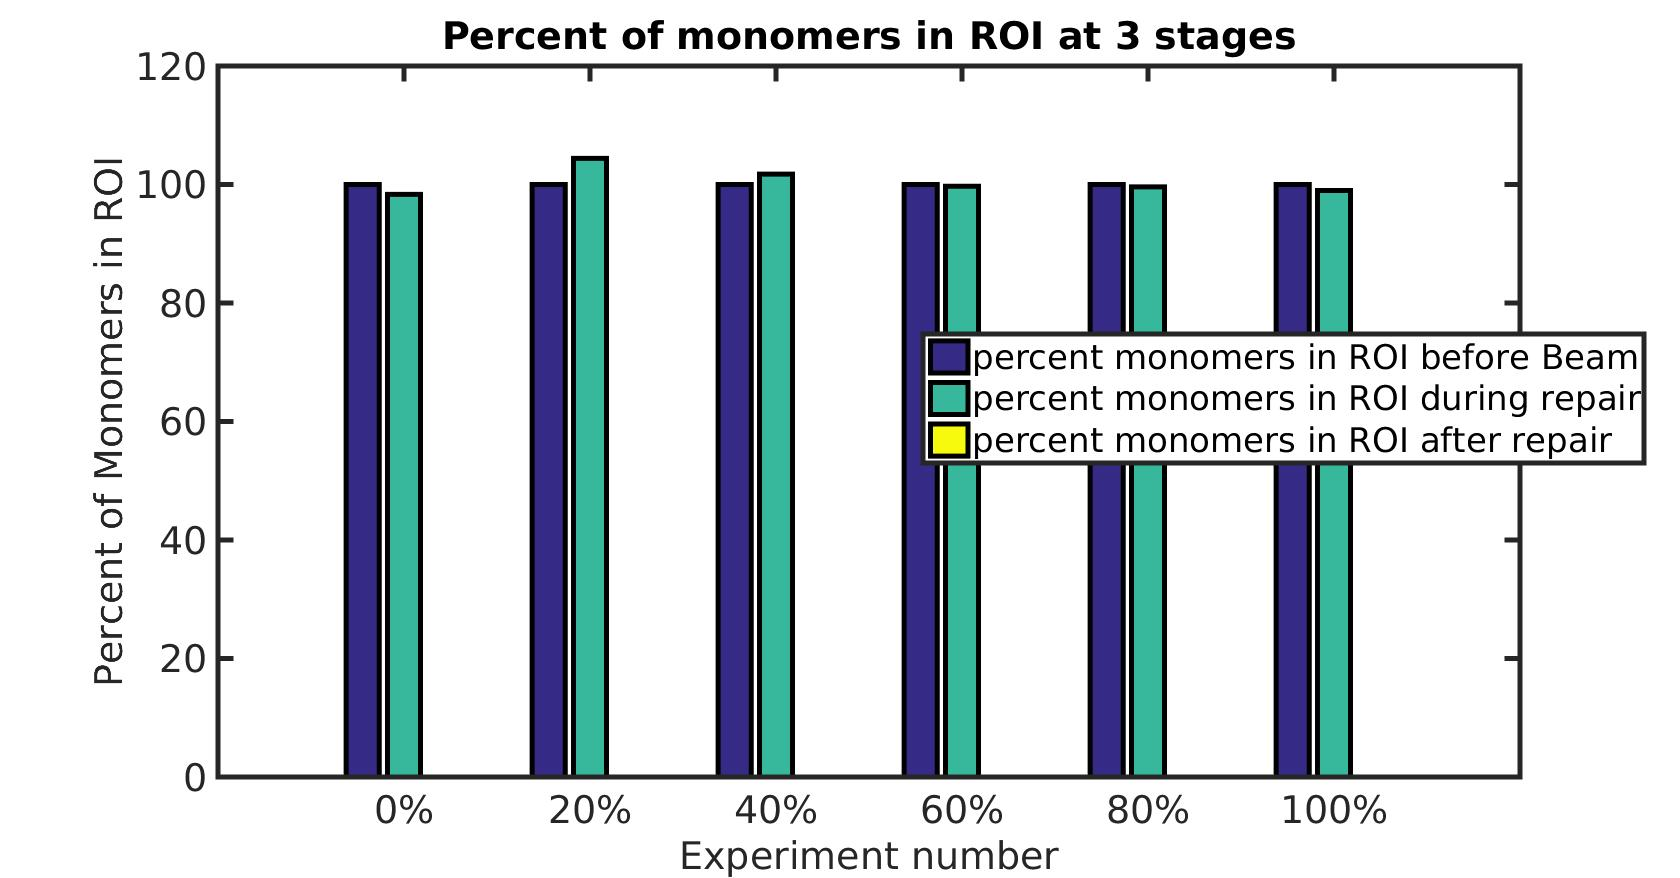
\includegraphics[width=0.5\linewidth, height=0.3\textheight]{Images/expandNonDamaged/NoCrosslinksBroken/percentageOfMonomersInROI}
	\caption{}
	\label{fig:meanNumMonomersInROINoBrokenCrosslinks}
	\end{figure}
    As can be seen in Figure \ref{fig:meanRadiusOfExpansionBendingNonAffecteNoBrokenCrosslinks}, the expansion of the damaged monomers is not stopped and it reaches that of the undamaged ones. The percentage of loss is accordingly small, since no monomers have left the ROI, which is determined by the damaged monomers radius of expansion. 
    
    
	\subsection{Assign bending to non-damaged monomers in the UVC beam}	
	 To simulate the process in which the repair mechanism proteins are recruited to the damage site, push away all non-damaged DNA and work on damage part, we assign bending elasticity force to monomers located within the damage region (beam) but those that were unaffected by the beam.
	 \subsubsection{Break damaged monomers' cross-links}
	 	 
	\begin{figure}[H]
	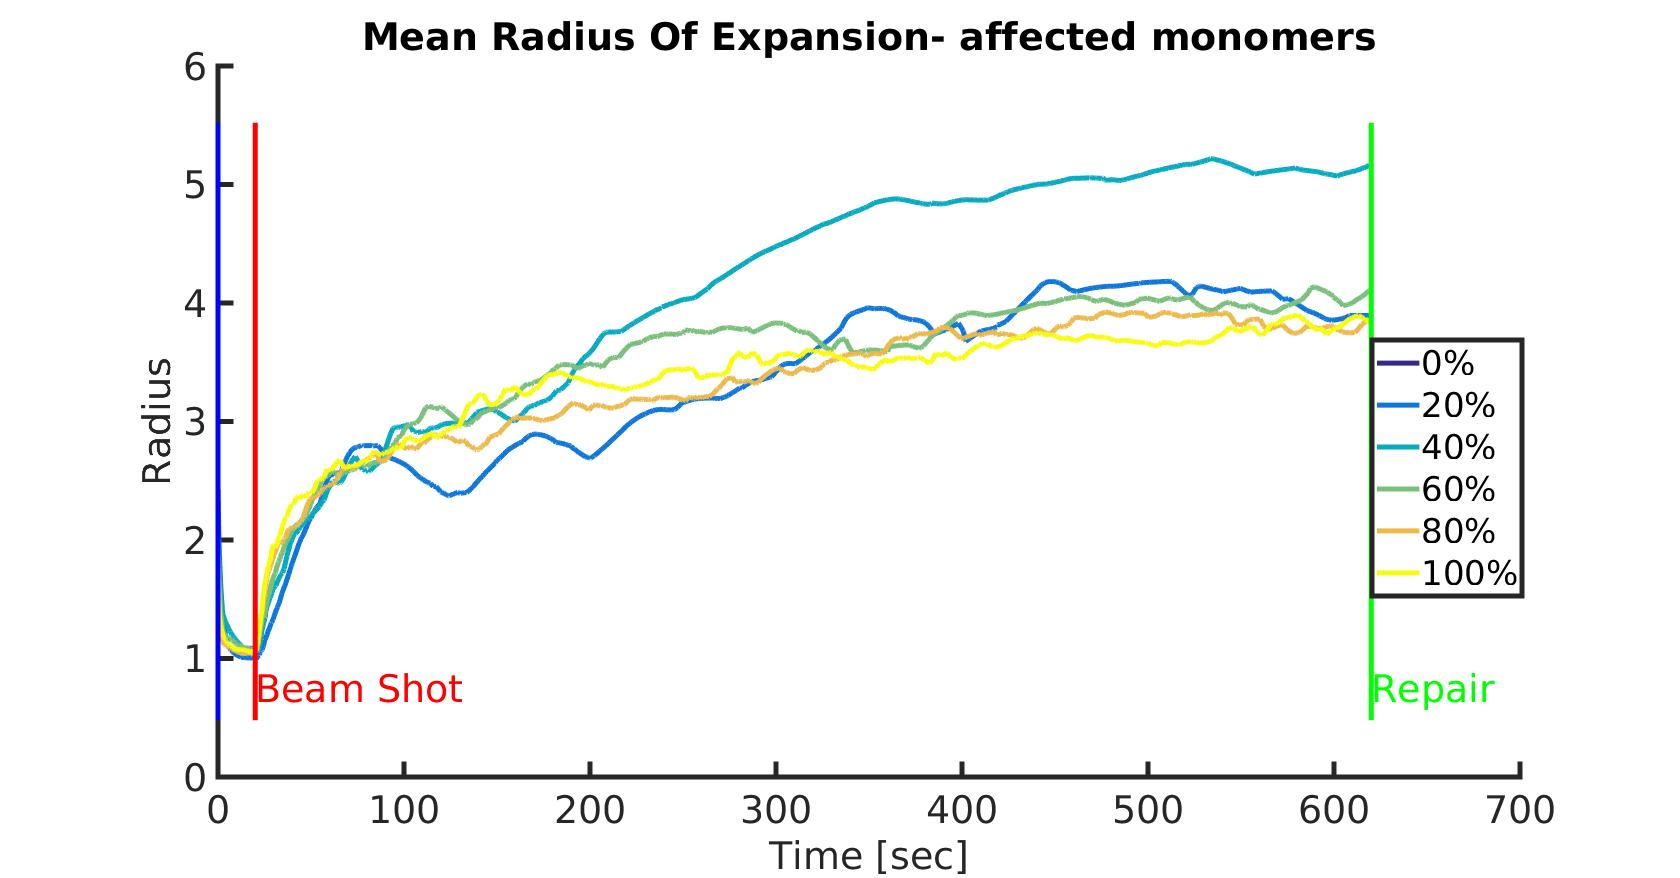
\includegraphics[width=0.5\linewidth, height=0.3\textheight]{Images/expandNonDamagedInBeam/breakDamagedCrosslinks/meanRadiusOfExpansionAffected}
	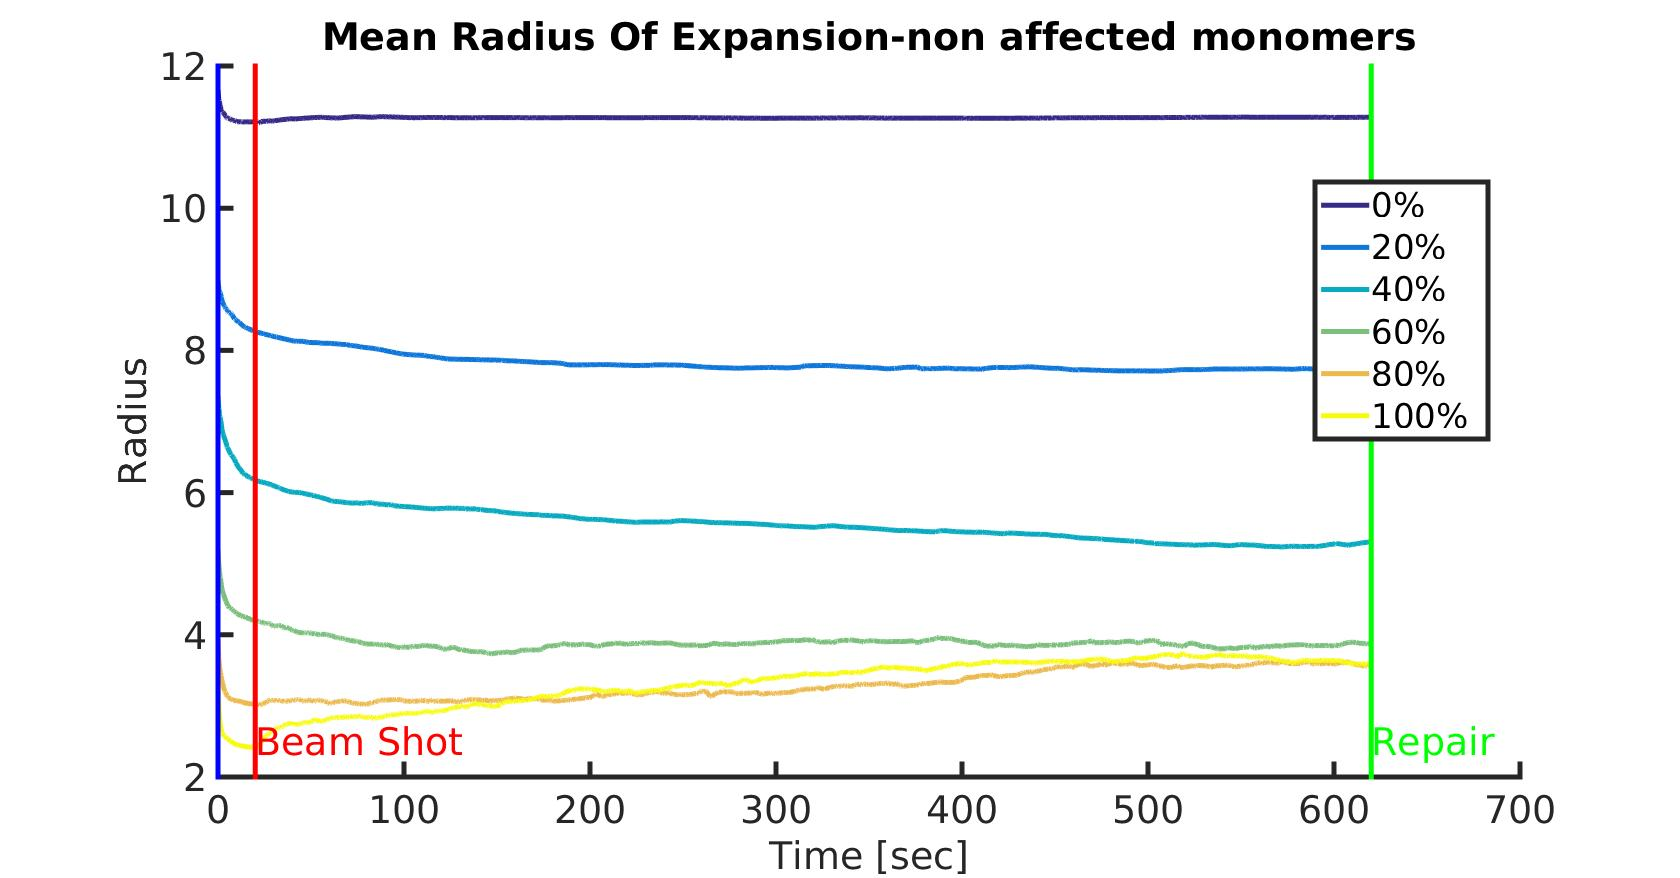
\includegraphics[width=0.5\linewidth, height=0.3\textheight]{Images/expandNonDamagedInBeam/breakDamagedCrosslinks/meanRadiusOfExpansionNonAffected}
	\caption{\tiny{\textbf{The radius of expansion for the affected (left) and the non-affected (right) monomers. The radius of the affected monomers expands roughly 3-times its initial value and converages to that of the non-affected monomers. There were non affected monomers in the case of 0\% conectivity, therefore the curve is not shown. (500 monomers, no Lennard-Jones, bending potential assigned to non-damaged monomers in the ROI)}}}
	\label{fig:meanRadiusOfExpansionAffected}
	\end{figure}
	 
	 \subsubsection{Keep all cross-links after UVC}
	 [Not tested]
	 
	 
	 \subsection{Region of exclusion around damaged monomers}
	 To simulate the arrival and crowding of repair mechanism in the damage site, we apply a mechanical pushing force around each damaged monomer after UVC beam shot. This force will operate in a finite range around each damaged monomers. Multiple force foci are updated simultaneously at each simulation step, where each force locus is placed on a damaged monomer. The force is derived from a truncated harmonic potential, and it acts as a spring at distances bellow its resting point at the exclusion radius. We test the expansion and DNA loss in the ROI similarly to the previous subsection. The ROI is determined according to the expansion of the damaged monomers, and we test two scenarios: one with cross-linked removed from and to the damaged monomer post UVC, and the second with all cross-links kept after UVC damage. 
     
     Description of the mechanical exclusion potential:
     \begin{equation*}
     U_m(r_i)= \frac{k_m}{2}\sum_{i,j}(R_e^2-\|r_i-c_j\|^2)^2 (H_0(\|r_i-c_j\|^2)-H_{R_m}(\|r_i-c_j\|^2)
     \end{equation*}
     where $R_m$ is the radius of force operation- above which the force zeros-out, $c_j$ is the $j^{th}$ force center, and $r_i$ is the position of the $i^{th}$ monomer. The function $H(x)$ is the Heaviside function.
     
     The force acting on monomers at each step as a result of the mechanical exclusion potential is similar to harmonic potential only truncated at a distance, which makes the harmonic potential repulsive.
     \begin{equation*}
     F_m=\frac{\partial U_m}{\partial r_i}=2k_m\sum_{i,j}(R_m^2-\|r_i-c_j\|^2)(r_i-c_j)(H_0(\|r_i-c_j\|^2)-H_{R_m}(\|r_i-c_j\|^2)
     \end{equation*}               
     
	 \subsubsection{Break damaged monomers' cross-links}
	 When we break the cross-links to and from damaged monomers post UVC
	 
	\begin{figure}[H]
	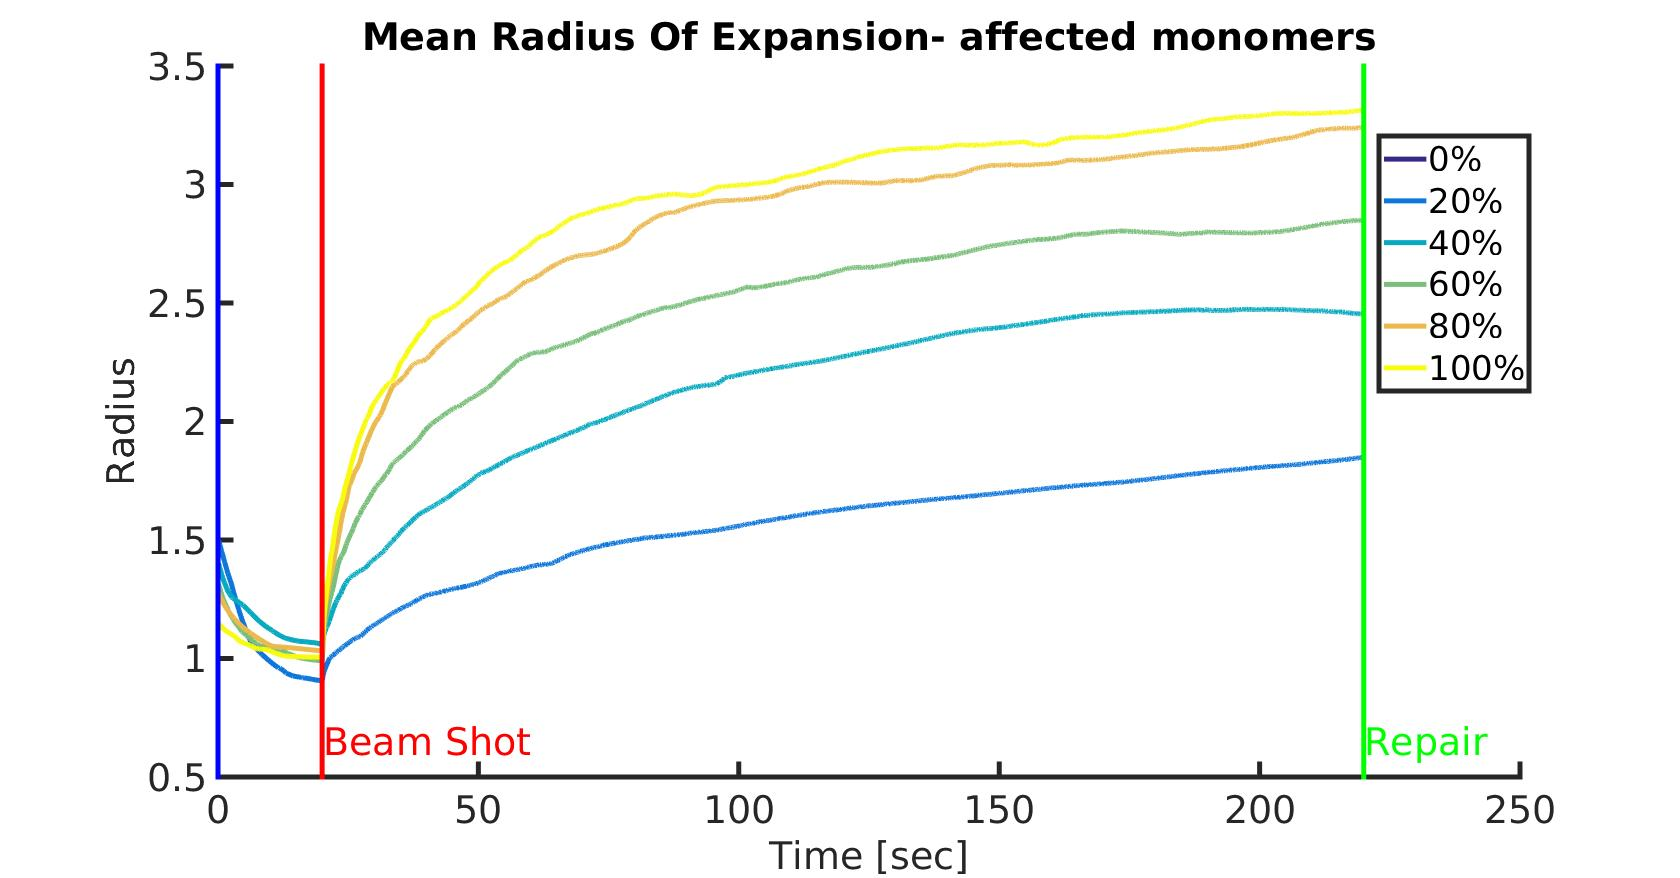
\includegraphics[width=0.5\linewidth, height=0.3\textheight]{Images/ExludeAroundDamagedMonomers/BreakDamagedCrosslinks/00/meanRadiusOfExpansionAffected}
		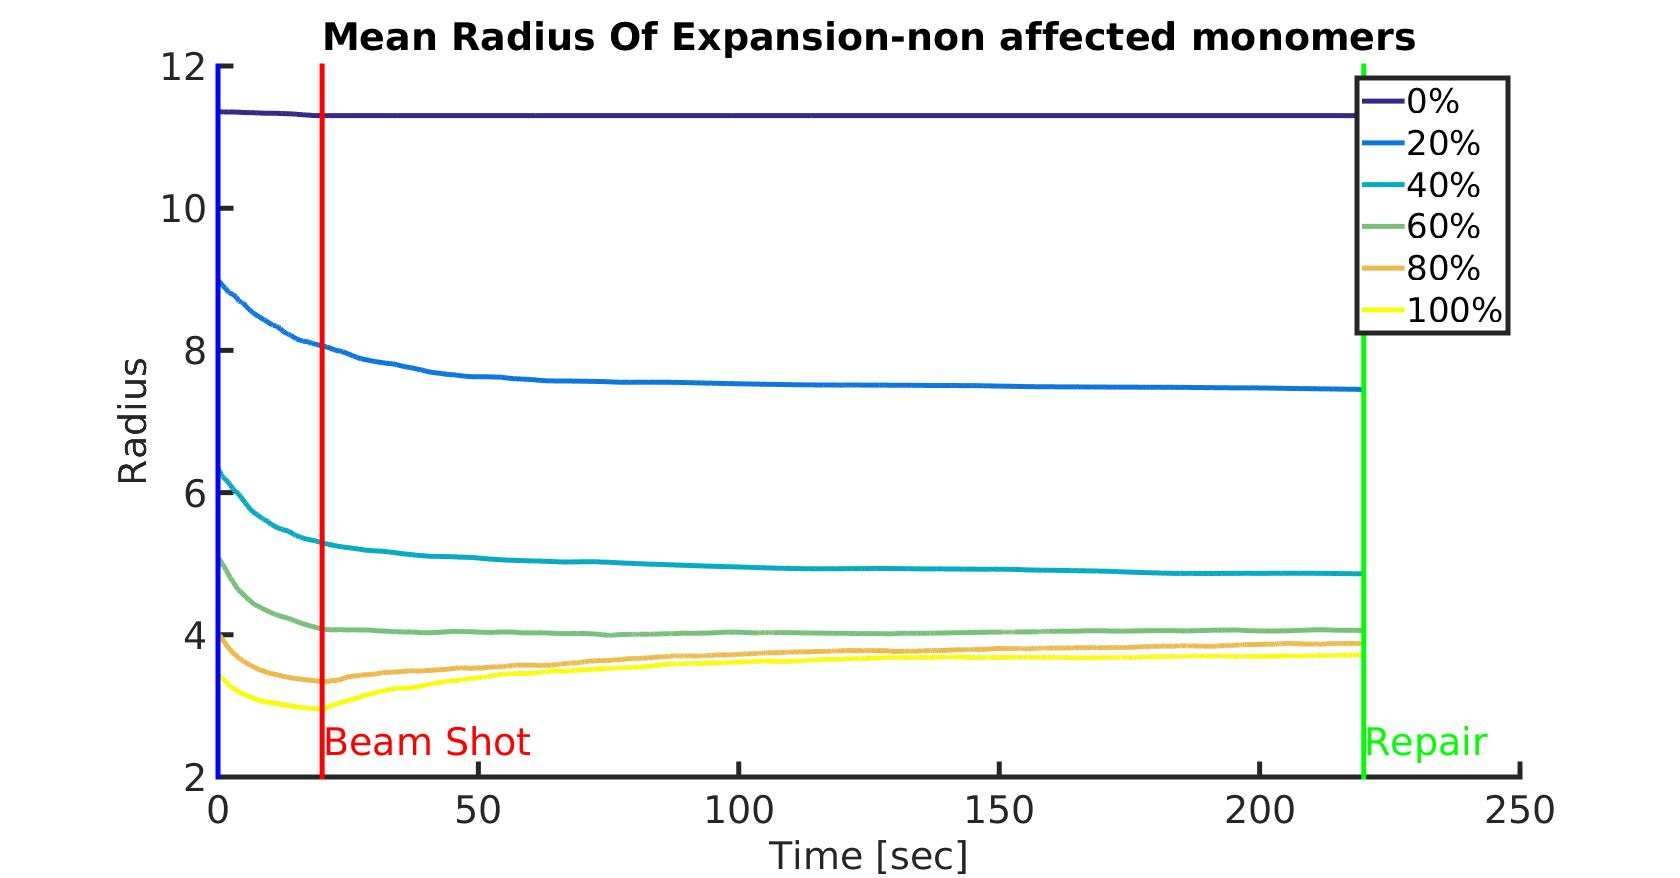
\includegraphics[width=0.5\linewidth, height=0.3\textheight]{Images/ExludeAroundDamagedMonomers/BreakDamagedCrosslinks/00/meanRadiusOfExpansionNonAffected}
	\caption{}
	\label{fig:meanRadiusOfExpansionAffectedVolumeOfExclusion}
	\end{figure}
	 In terms of DNA loss in the ROI
	 
	\begin{figure}[H]
	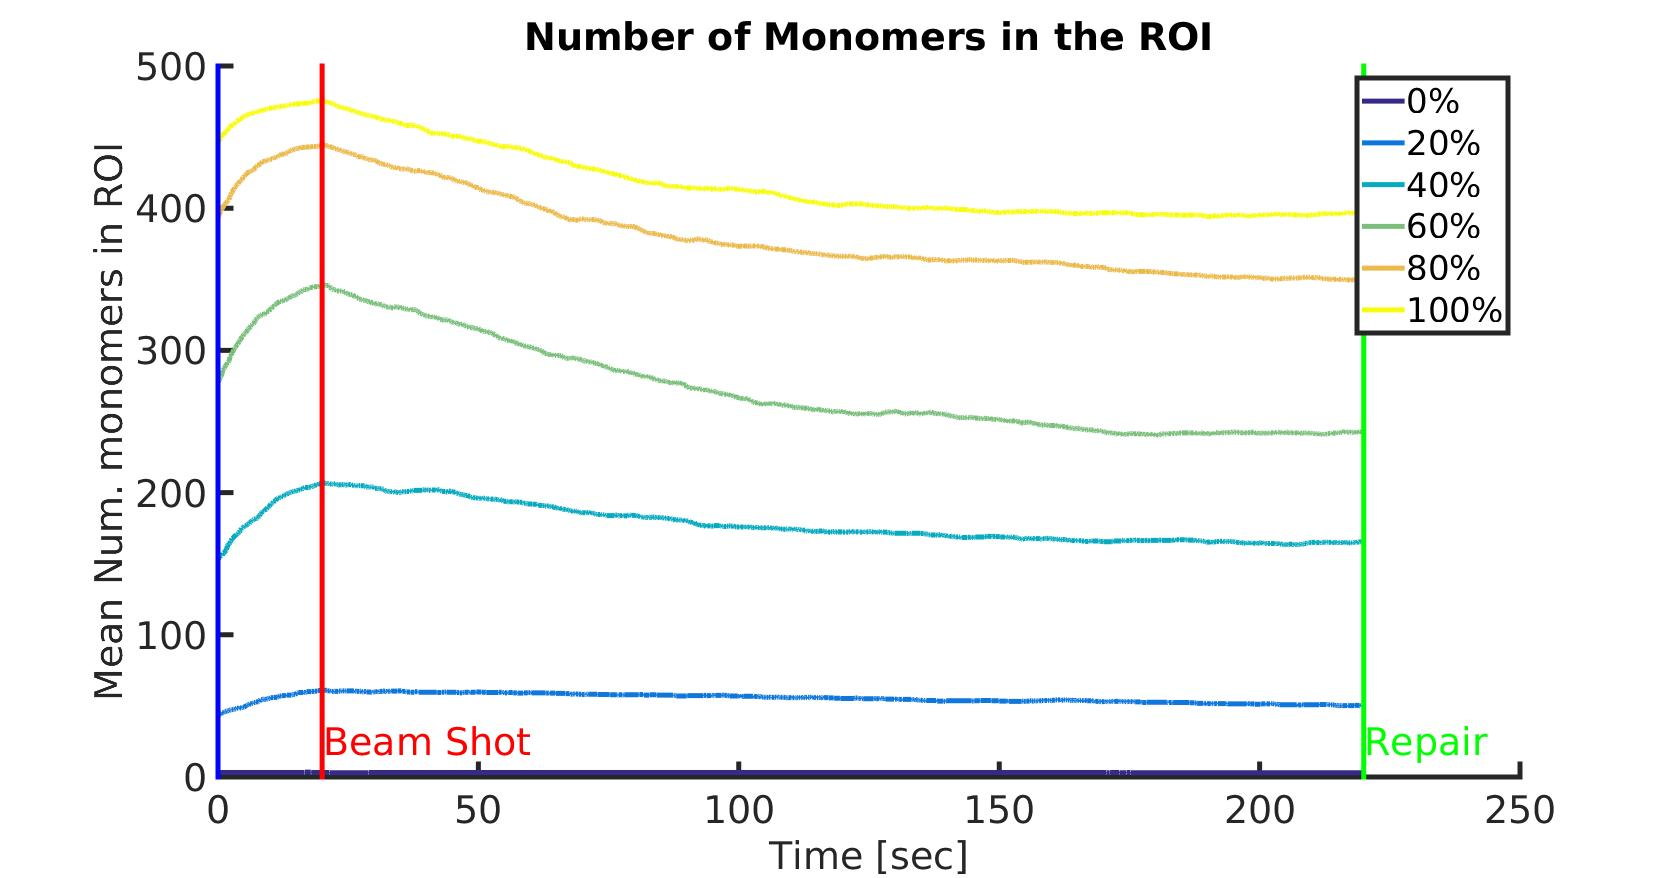
\includegraphics[width=0.5\linewidth, height=0.3\textheight]{Images/ExludeAroundDamagedMonomers/BreakDamagedCrosslinks/00/meanNumberOfMonomersInROI}
	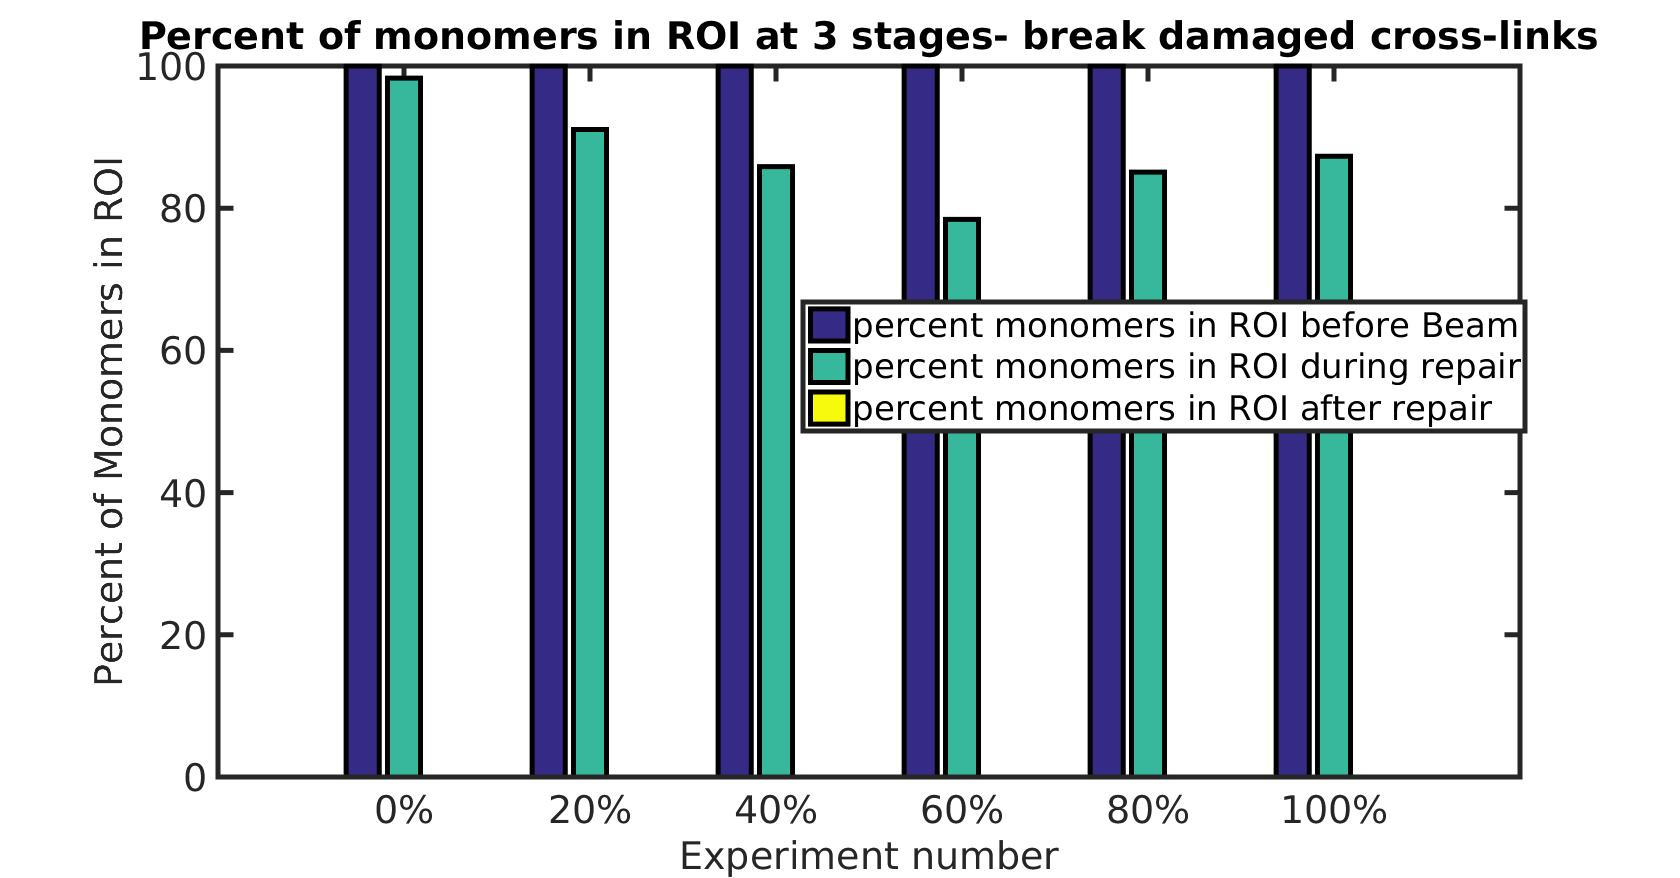
\includegraphics[width=0.5\linewidth, height=0.3\textheight]{Images/ExludeAroundDamagedMonomers/BreakDamagedCrosslinks/00/percentOfMonomersInROI}
	\caption{The number of monomers in the ROI (left) and the overall percentage of monomer loss (right) at the end of repair stage for various percentage of cross-linking.}
	\label{fig:meanNumberOfMonomersInROIVolumeOfExclusion}
	\end{figure}
	 
	 
	 \subsubsection{No cross-links broken}
	 When we do not break the cross-links to and from the damaged monomers post UVC, result show:
	 	 
	\begin{figure}[H]
	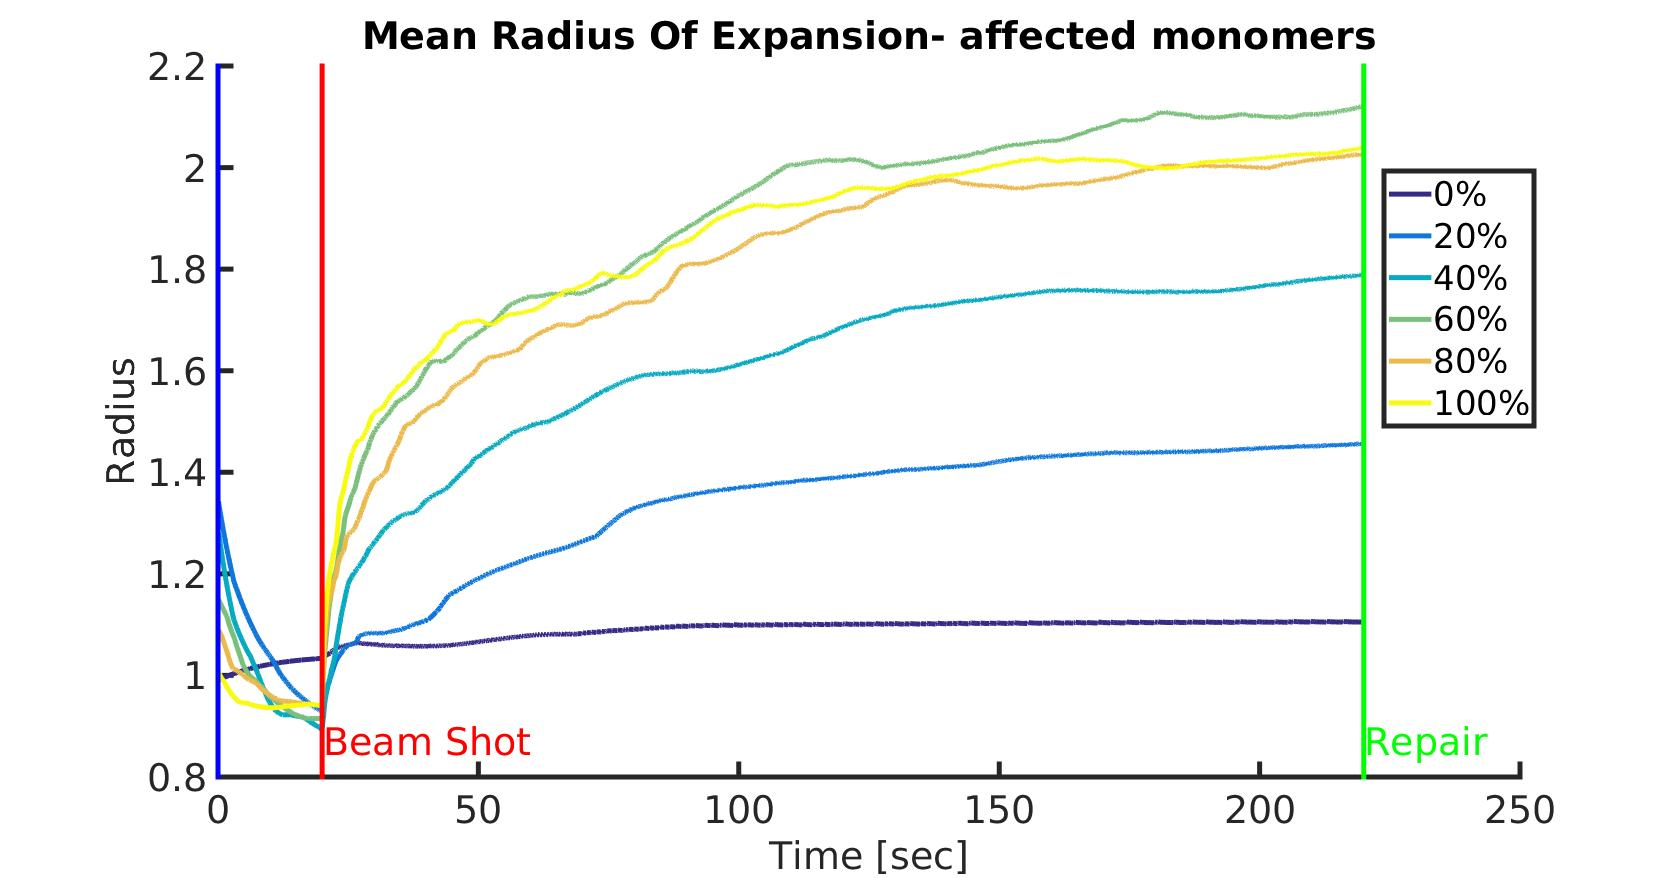
\includegraphics[width=0.5\linewidth, height=0.3\textheight]{Images/ExludeAroundDamagedMonomers/NoCrosslinksBroken/00/meanRadiusOfExpanssionAffected}
	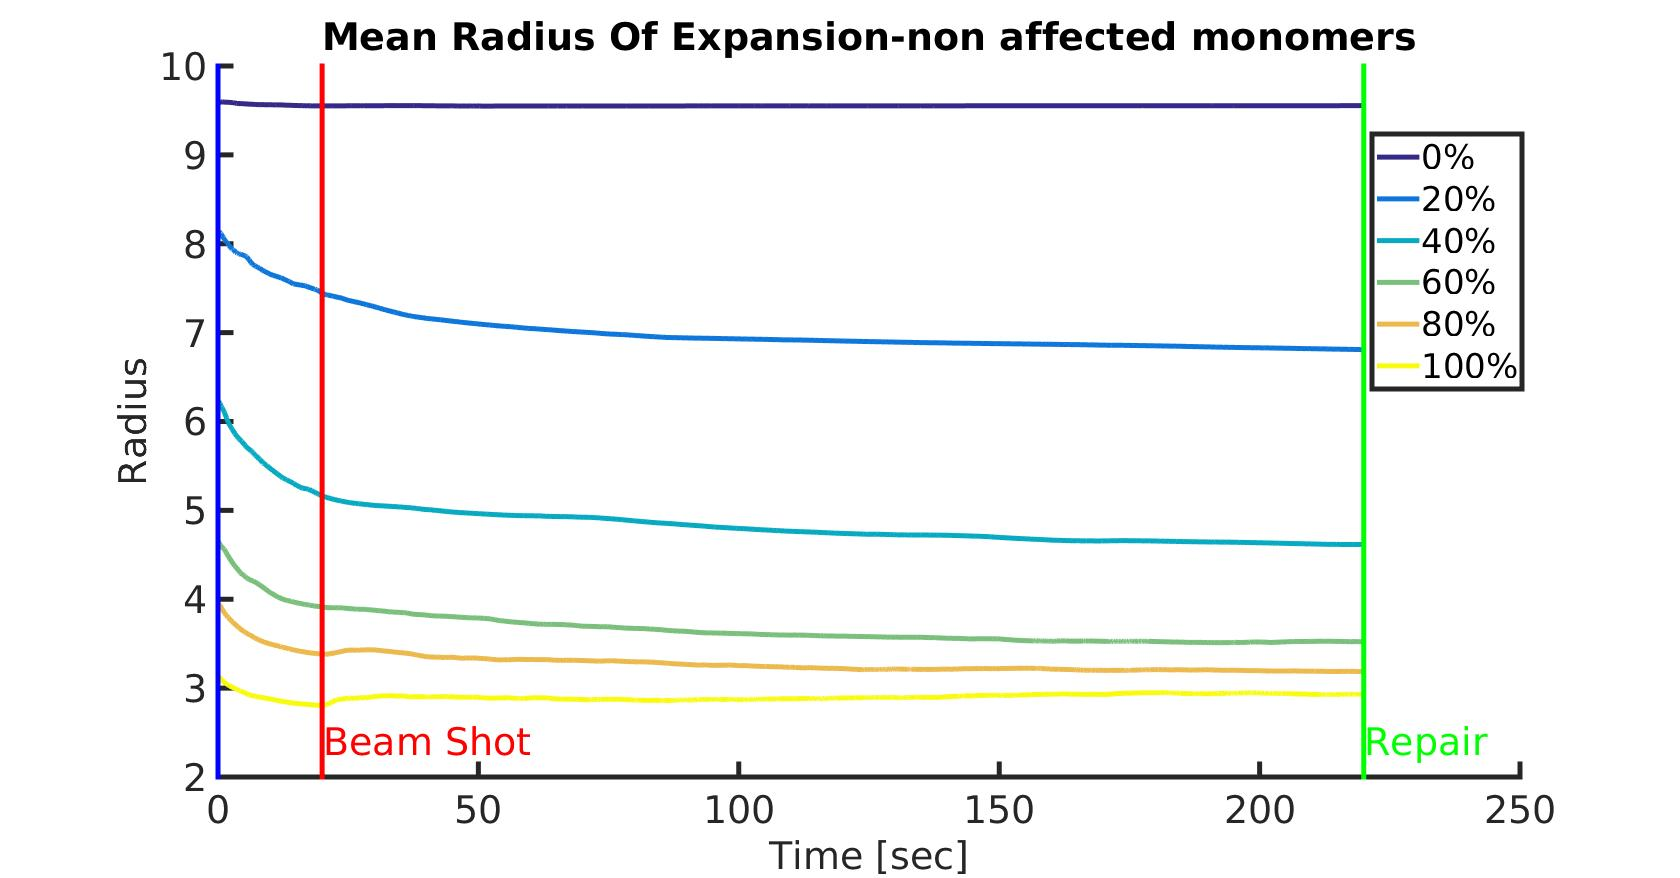
\includegraphics[width=0.5\linewidth, height=0.3\textheight]{Images/ExludeAroundDamagedMonomers/NoCrosslinksBroken/00/meanRadiusOfExpanssionNonAffected}
	\caption{\tiny{\textbf{The mean radius of expansion for the damaged (left) and non-damaged (right) monomers for different percentage of cross-linking. Post UVC a circle of exclusion is drawn around the position of each damaged monomers and a pushing force is applied to all monomers located within the circle. . this force serves to simulated the recruit and crowding of the repair mechanism at the damage site. The radius of expansion of the damaged monomes converges for all percentages of cross-linking and never exceeds those of the non-damaged.in all cases, the expansion converges to roughly twice that of the initial radius of expansion at UVC initiation. (400 monomers. No Lennard-Jones, no bending potential, all cross-links are kept post UVC)}}}
	\label{fig:meanRadiusOfExpanssionAfectedVolumeOfExclusion}
	\end{figure}
	
	In terms of the DNA loss, we get 	
	\begin{figure}[H]
	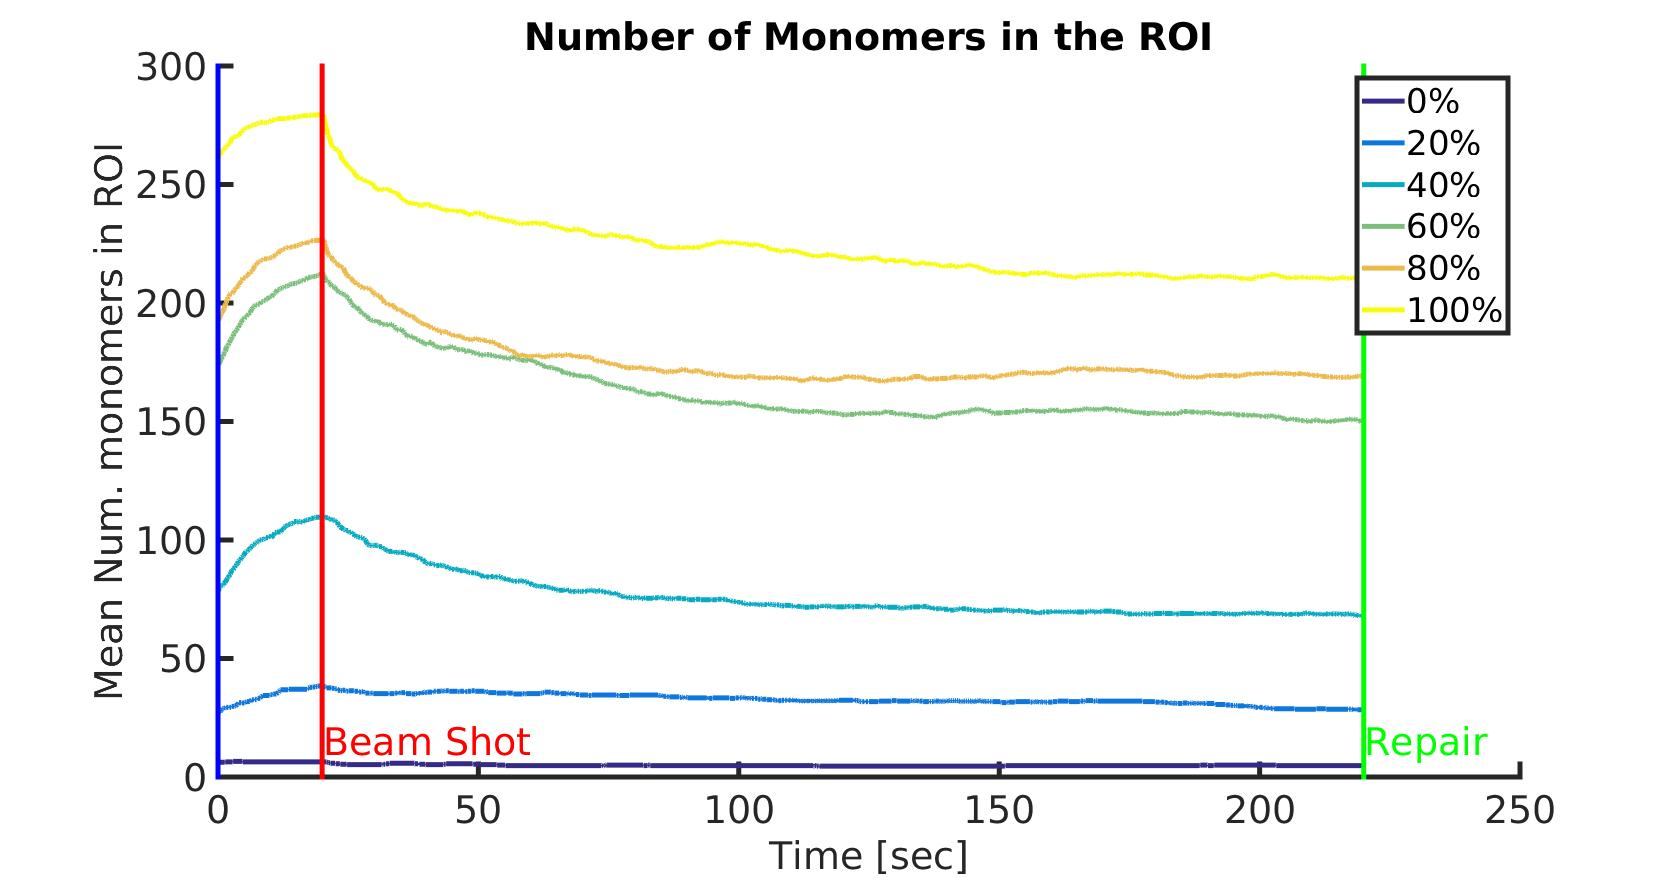
\includegraphics[width=0.5\linewidth, height=0.3\textheight]{Images/ExludeAroundDamagedMonomers/NoCrosslinksBroken/00/meanNumMonomersInROI}
	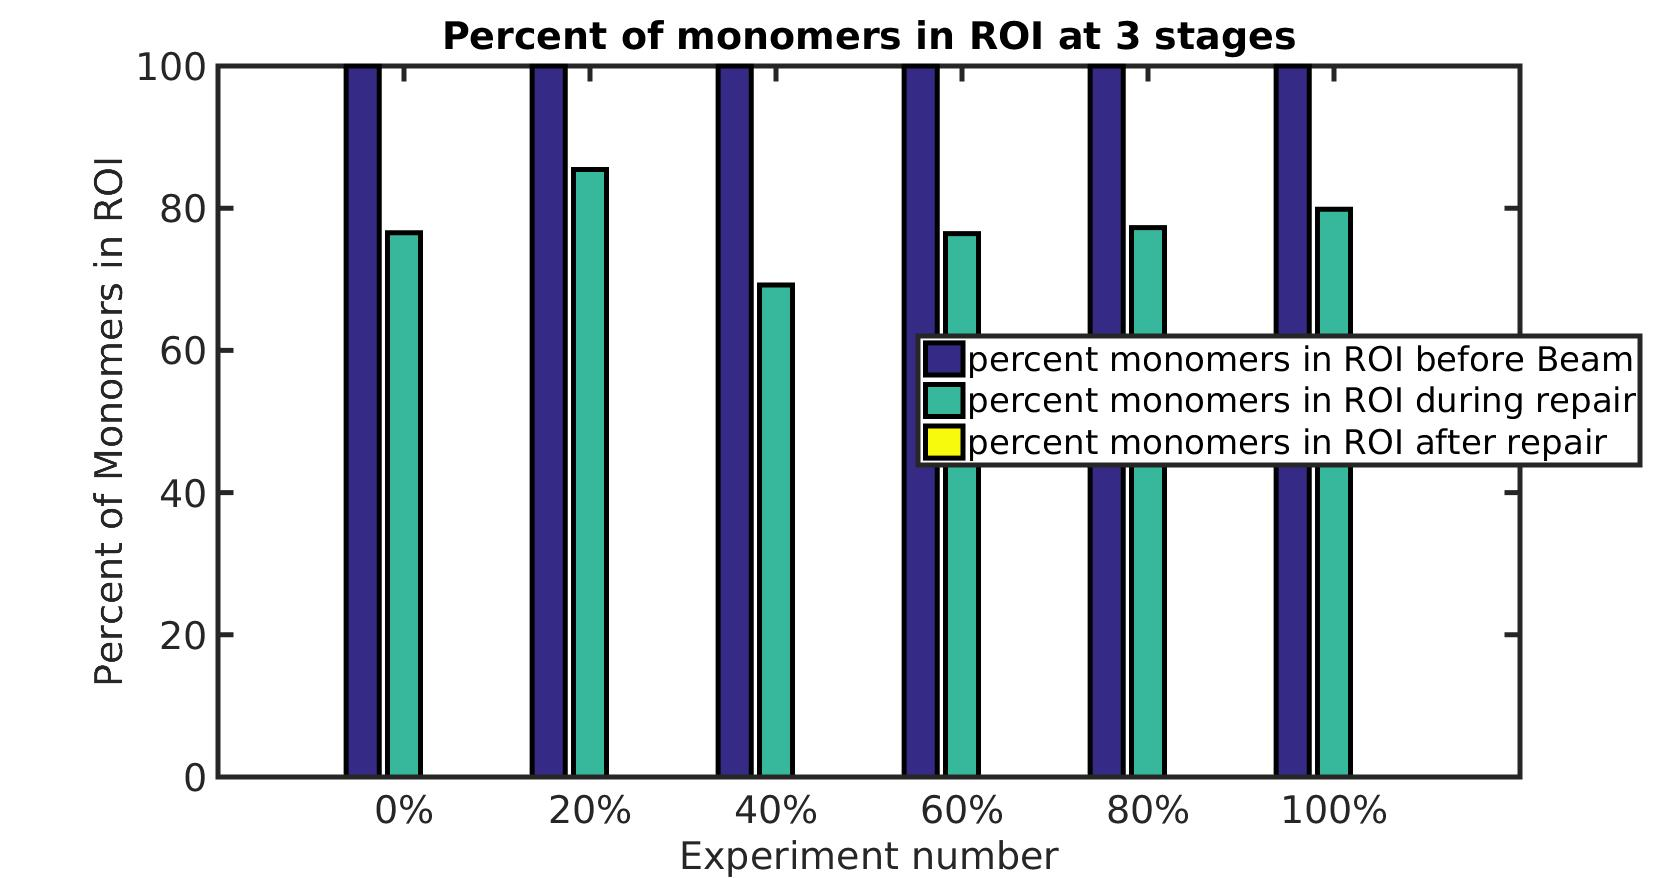
\includegraphics[width=0.5\linewidth, height=0.3\textheight]{Images/ExludeAroundDamagedMonomers/NoCrosslinksBroken/00/percentOfMonomersInROI}
	\caption{\tiny{\textbf{The absolute number of monomers in the ROI (left) and the percentage of loss at the end of simulation (right). For low degree of connectivty we have little to no change in the number of monomers in the ROI. Low level of conectivity turns out to be less reliable due to the fact that initialy less monomes are located near the center of mass of the polymer, where the beam is shot through. For high degree of connectivity (60-100\%, we see decrease roughly around 20\%. (400 monomers. No Lennard-Jones, exclusion around damaged monomers. no bending potential. All cross-links are kept post UVC)) }}}
	\label{fig:meanNumMonomersInROIVolumeOfExclusion}
	\end{figure}
	
	
	
  \subsubsection{Parameter fitting}
   \textbf{The radius of Exclusion} \\
  
   From the result of simulating the process with cross-links broken for the damaged monomers, we see that ~20\% loss of DNA can be achieved for 60-80\% connectivity. However, the radius of expansion tends to be roughly 3 times the initial radius, which do not agree with experimental observations. In experiments the damaged area (repair zone) expands three-folds in area, which is $\sqrt{3}$ in radius. We now take 80\% connectivity and explore the values of the exclusion volume around each damaged monomer and the expansion constant and fit them to experimental observations. 
   
   We vary the value of the radius of exclusion around damaged monomers from 0.6 to $\sqrt{2}/2$ while keeping 80\% cross-linking. 
   
   
	\begin{figure}[H]
	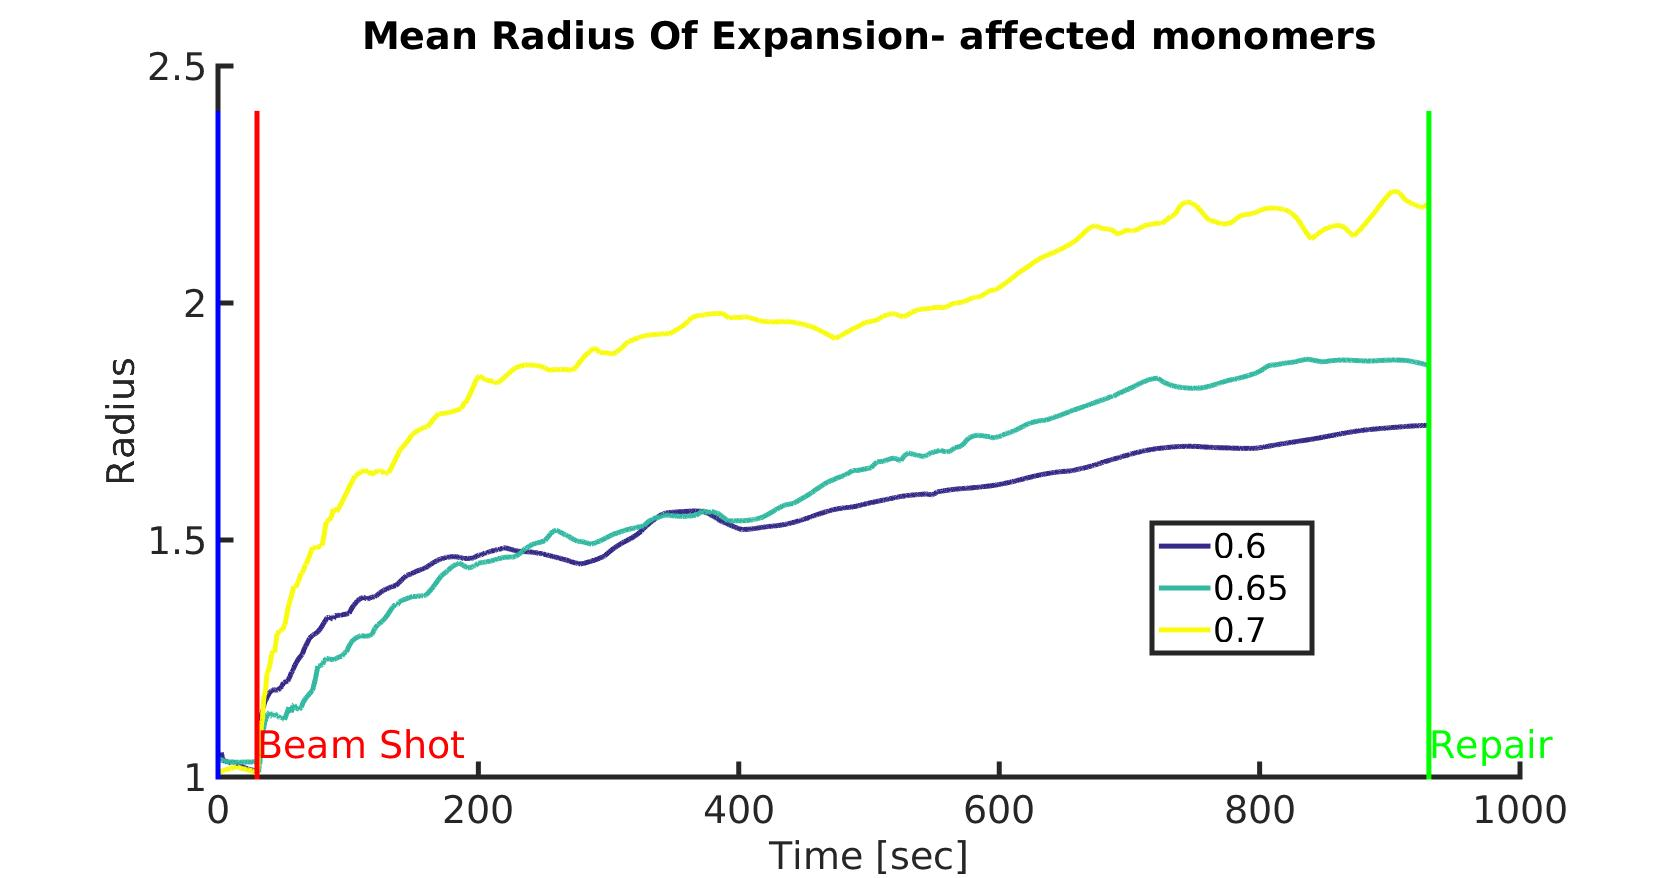
\includegraphics[width=0.5\linewidth, height=0.3\textheight]{Images/ExludeAroundDamagedMonomers/BreakDamagedCrosslinks/06/meanRadiusOfExpansionAffected}
	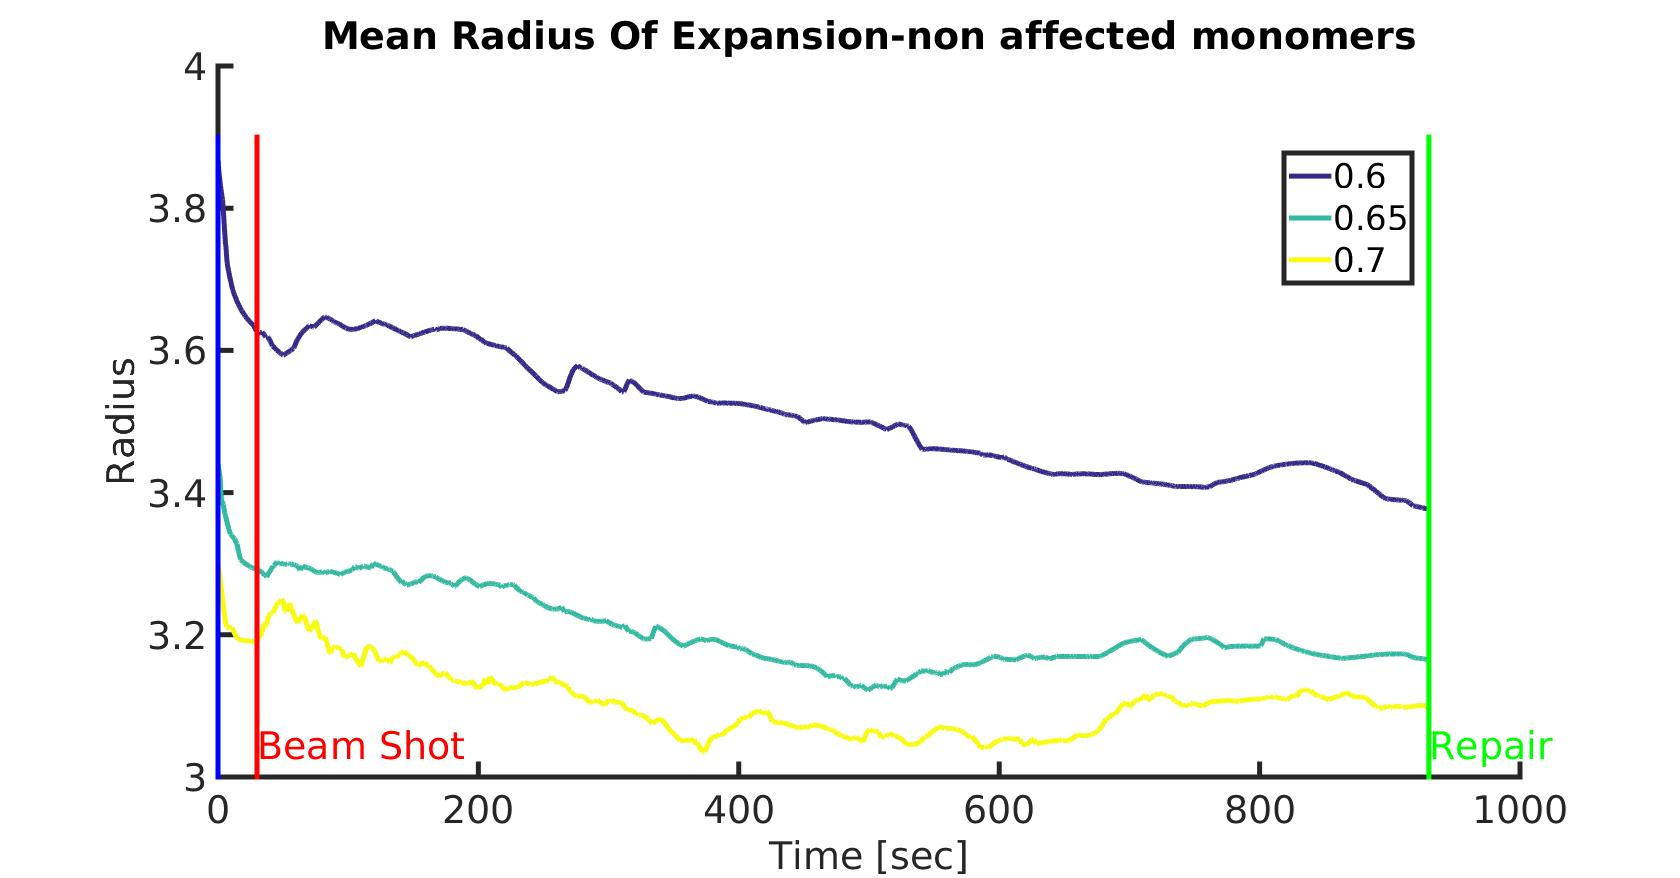
\includegraphics[width=0.5\linewidth, height=0.3\textheight]{Images/ExludeAroundDamagedMonomers/BreakDamagedCrosslinks/06/meanRadiusOfExpansionNonAffected}
	\caption{\tiny{\textbf{Mean radius of expansion for the damaged (left) and non-damaged (right) monomers for 3 values of radius of exclusion around damaged monomers (legend). The cross links to and from each damaged monomers were removed post UVC. An expansion of ~1.7 is observed for radius of 0.65 (blue curve). The polymer included 500 monomers. 3 replicas of the experiment were made for each value of exclusion radius. simulation were performed for 9000 steps with a time step of 0.1, which results in 15 minuts.}}}
	\label{fig:meanRadiusOfExpansionAffectedVolumeOfExclusionParameterFitting}
	\end{figure}
   
   The number of monomers in the ROI remained stable for all 3 values of the radius of exclusion.
   
	\begin{figure}[H]
	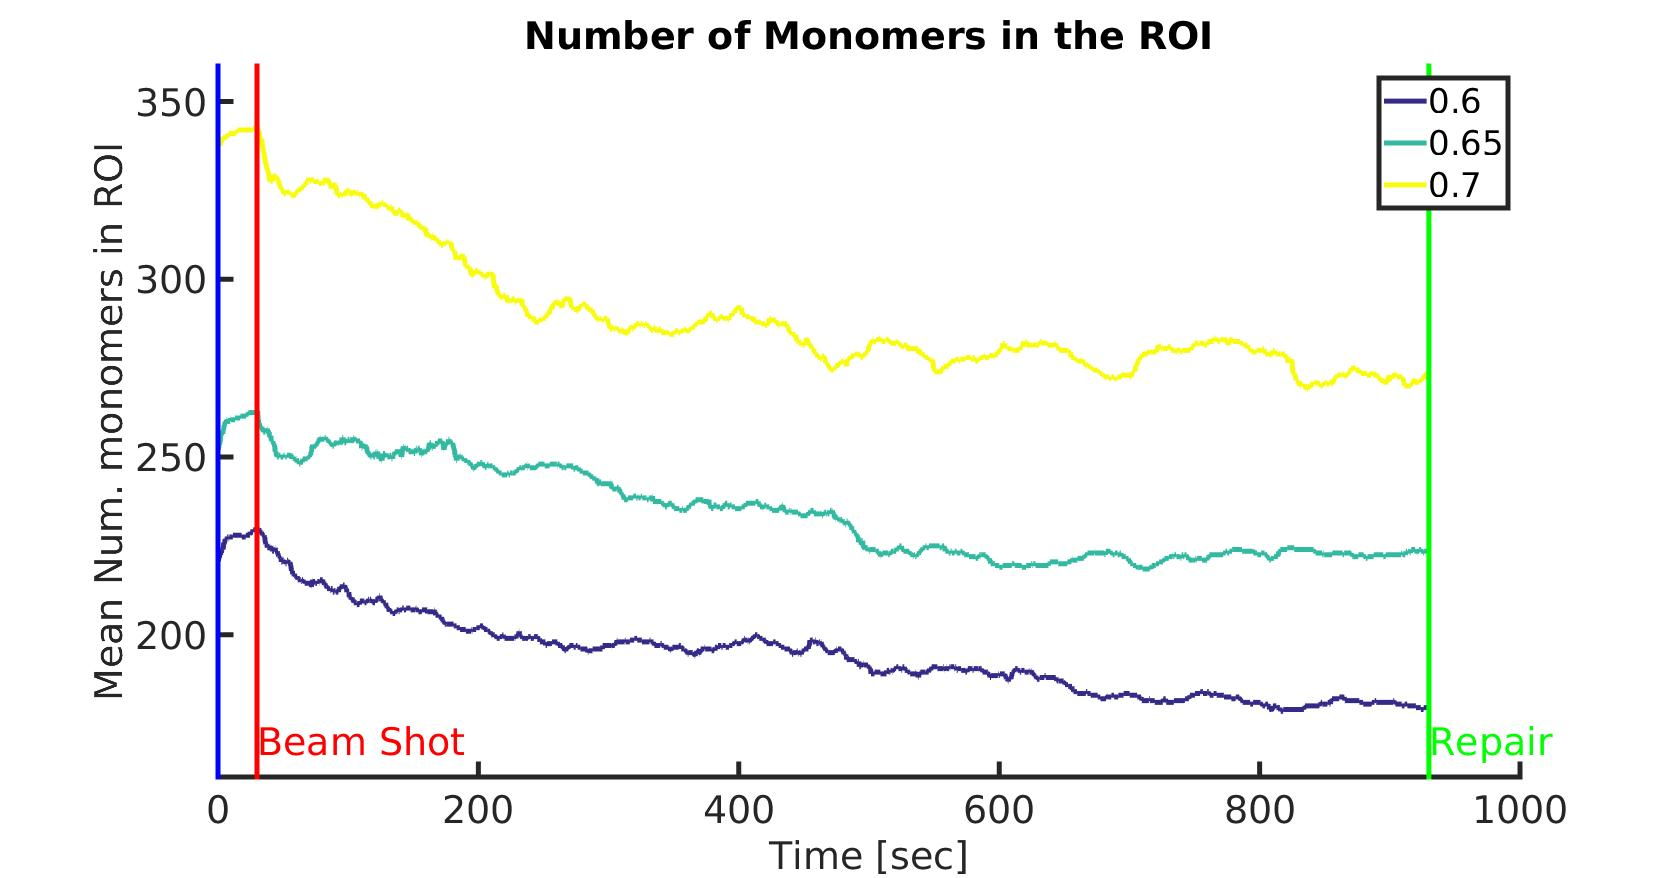
\includegraphics[width=0.5\linewidth,height=0.3\textheight]{Images/ExludeAroundDamagedMonomers/BreakDamagedCrosslinks/06/meanNumMonomersInROI}
	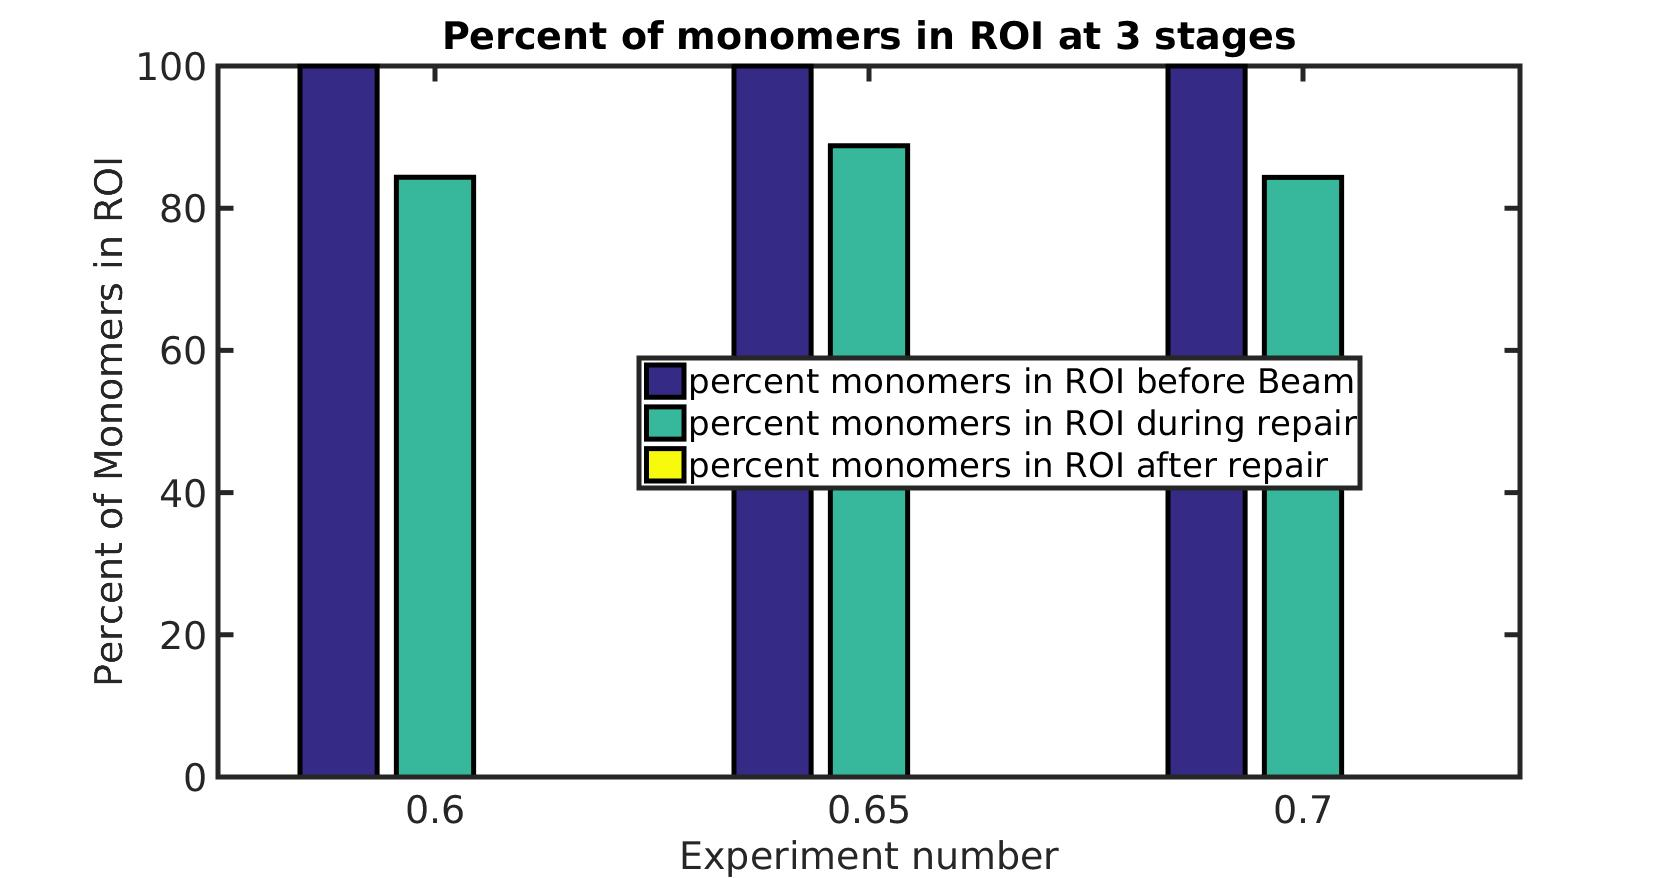
\includegraphics[width=0.5\linewidth,height=0.3\textheight]{Images/ExludeAroundDamagedMonomers/BreakDamagedCrosslinks/06/percentOfMonomersInROI}
	\caption{\tiny{\textbf{The mean number of monomers in the ROI (left) and their percentage out of the total (right) for 3 values of the exclusion volume shows stability in the loss percentages (mean of 3 replicas). However, the value 0.65, which showed a radius of expansion 1.7 times the initial radius of the damaged monomerrs (see previous figure) has shown a slightly lower loss percentages than the others. This could be a result of the few experiments performed. more replicas might be needed. the polymer includede 500 monomers and ran for 900 step with time step of 0.1 second}}}
	\label{fig:meanNumMonomersInROIVolumeOfExclusionParameterFitting}
	\end{figure}
	   
   We see from the figures above that a radius of exclusion $R_e=0.6$ provides us with an expansion of roughly $\sqrt{3}$, and allow 20\% loss of monomers from the ROI. \\
         
   \textbf{\large{Relationship between radius of exclusion and expansion}}   
   In essence, we should be able to predict the magnitude of the radius of expansion if we know the number of monomers damaged due to UVC in the volume exclusion model. 
   The redius of expansion of the damaged monomers should depend on the radius of the UVC beam, the total number of monomers and the probability of a monomer to be damaged (time of UVC exposure).
   An exclusion around each damaged monomers converges over time to a geometrical arrangement with damaged monomers roughly equidistant from one another. Assuming equidistant (mean) model, we assume the expansion of damaged monomers to be in a square region rather than a circular (see figure), and we approximate the radius of expansion to be half the diagonal of this square region. Therefore, the relationship between the radius of expansion, the number of monomers, the UVC beam radius and the radius of exclusion should roughly follow
   \begin{equation*}
   \left[\frac{[pNF_{cm}^c(R_b)]^{0.5}}{2}-1 \right]R_e = R_b\alpha
   \end{equation*}
   
   with $N$ the number of monomers,$R_b$ the radius of the UVC beam, $F_{cm}^c(R_b)$ the probability function for a monomer to be at a distance less than $R_b$ from the center of mass with cross-linking percentage $c$, $R_e$ the radius of exclusion around each damaged monomer,$p$ the probability of a monomer to be damaged given its distance from center-of-mass, and $\alpha$ is the ratio between the radius of expansion at the end of repair stage and that at initiation of UVC beam, and is based on experimental observations. Note that $NF_{cm}^c(R_b)$ is the expected number of monomers in the region around the center of mass. 
   
	\begin{figure}][H]
	\centering
	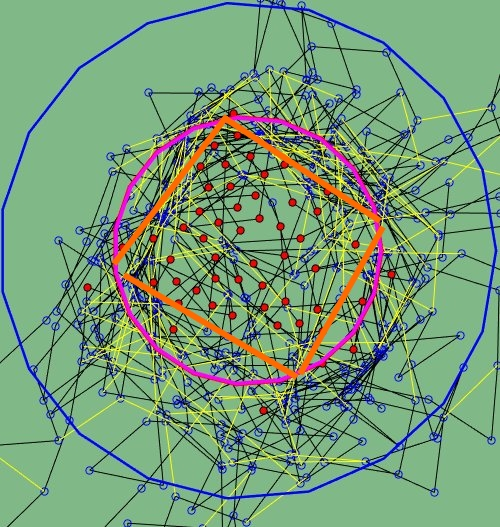
\includegraphics[width=0.4\linewidth]{Images/ExludeAroundDamagedMonomers/BreakDamagedCrosslinks/testExpansion/snapshotForExampleOfExpansionEstimation}
	\caption{\tiny{\textbf{A snapshot from one of the siulaton depicting the square approximatino to the distribution of the damaged monomers (red circles). The damaged monomers (red) expand to a circle (magenta) at the end of simulation. The Orange lines are hand drawn to depict the approximation of the radius of expansion with half the diagonal of this rectangle. A model with 500 monomers and 80\% crosslinking}}}
	\label{fig:snapshotForExampleOfExpansionEstimation}
	\end{figure}
   We do not have direct access to the probability density of monomers in a cross-linked polymer and so $F_{cm}^c$ is at the moment unknown. However, we noe empirically that with the parameters we chose, the expected number of monomers hit by UVC is 10\% of the total number of monomer, $N$ (given the UVC radius is 1). 
   
   The radius of the damaged monomers at initiation of UVC is roughly equivalent to that of the beam, because the probability of a monomer to be damaged is high.  But in general, damage probability follows a Gaussian distribution. Therefore, to be more accurate, we replace $R_b$ with the standard deviation of the Gaussian $\sigma_{b}$. This brings us to 
    
    \begin{equation*}
    \left[\frac{[pNF_{cm}^c(\sigma_b)]^{0.5}}{2}-1 \right]R_e = \sigma_b\alpha
    \end{equation*}
    
   To complete the calculation, it remains to evaluate $F_{cm}^c(\sigma_b)$, which will be dealt with later.
   
   \textbf{Example}:\\
   To estimate the value of the radius of exclusion for damaged monomers in a 500 monomer chain, such that the radius of expansion for the damaged monomers will increase $\alpha =\sqrt{3}$ its initial size (as observed in experiments), We assume that the UVC beam radius is $R_b=1$. Following the first approximation, with  $pNF_{cm}^c(R_b)=50$ we get 
   \begin{equation*}
   R_e =2\sqrt{3}/(\sqrt{50} -2) = 0.68
   \end{equation*}
   plugging $R_e=0.68$ in our simulations we get
   
	\begin{figure}[H]
	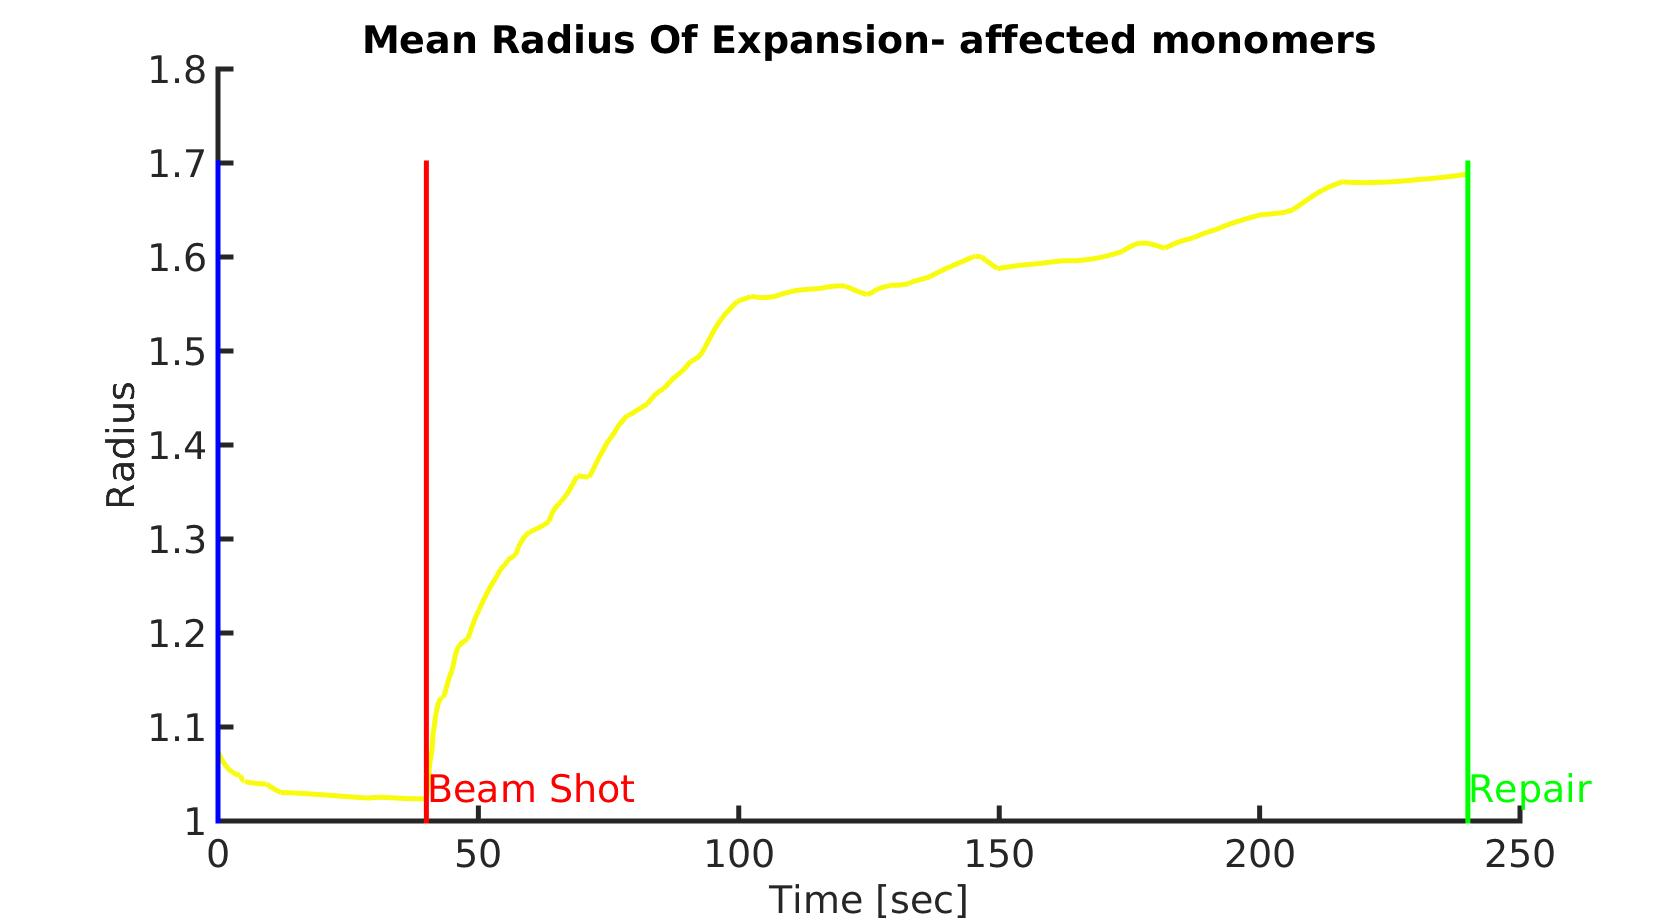
\includegraphics[width=0.5\linewidth, height=0.3\textheight]{Images/ExludeAroundDamagedMonomers/BreakDamagedCrosslinks/testExpansion/meanRadiusOfExpansionDamagedMonomers}
	\caption{\tiny{\textbf{validating prediction of radius of expansion. Plugging $R_e=0.68$ in a model with 500 monomers and beam radius of 1 $\mu$m, we see that the simple approximation made in this section fits excellently to the observations. Over time the radius has expanded to $\sqrt{3}$ time its initial value of 1}}}
	\label{fig:meanRadiusOfExpansionDamagedMonomers}
	\end{figure}
	 Although we see good agreement with simulations, the percent of monomers lost the ROI in this model with $R_e=0.68$ in about 30\% at the end of repair stage.
	 
	\begin{figure}[H]
	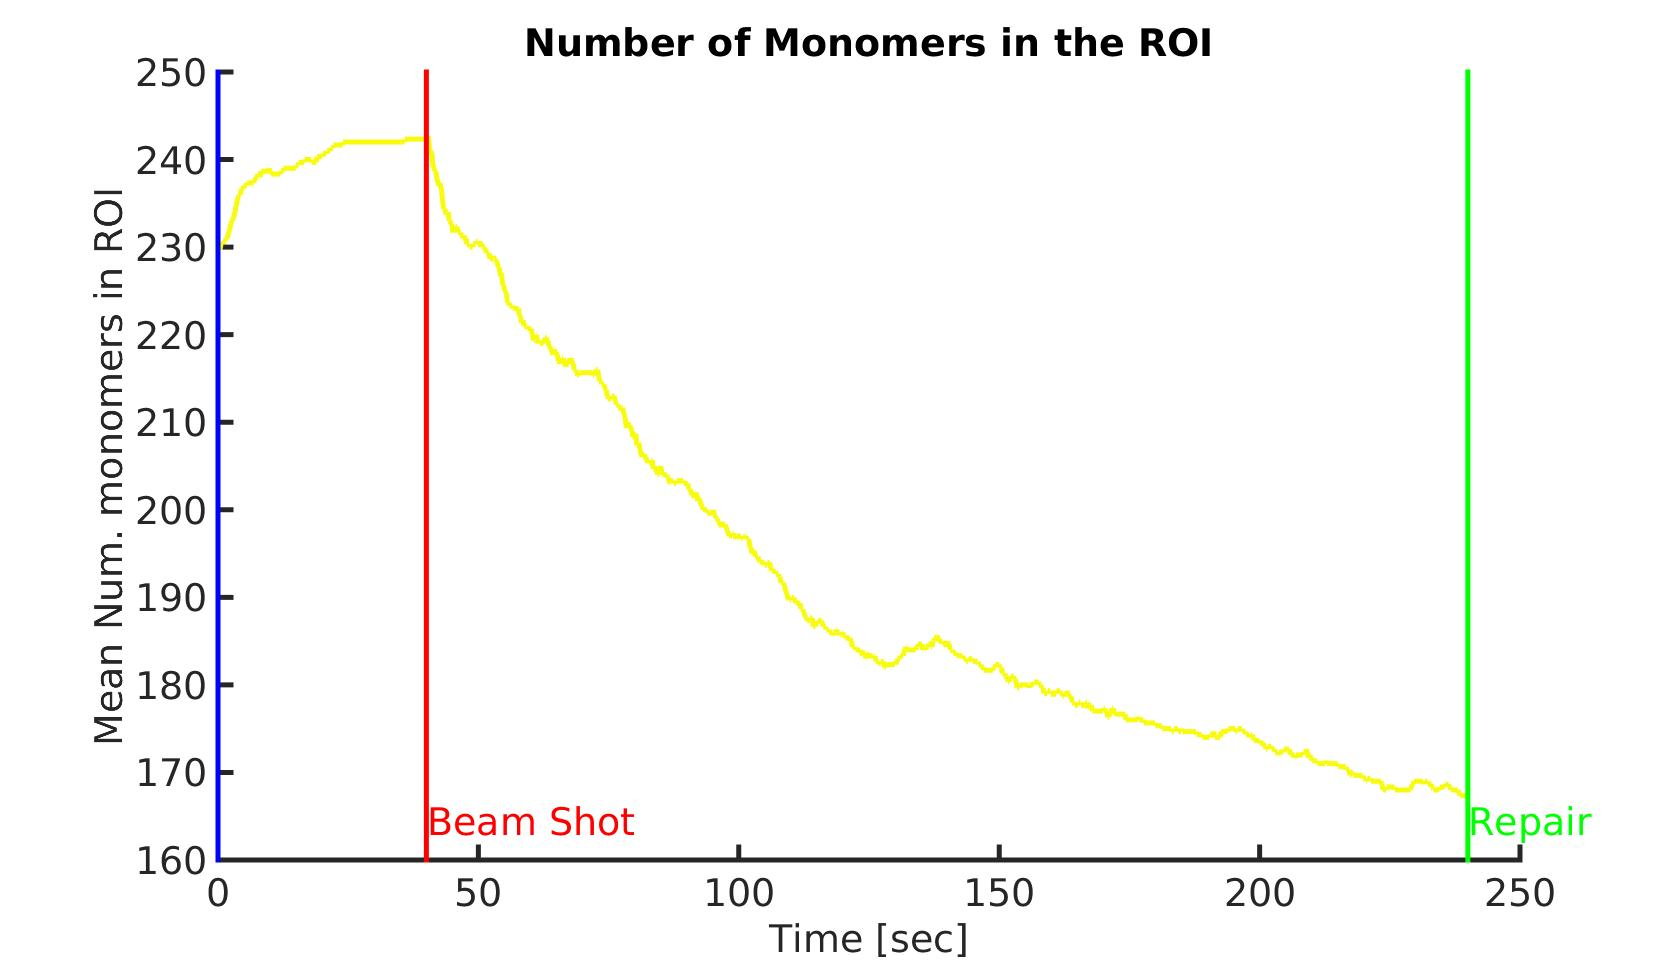
\includegraphics[width=0.5\linewidth, height=0.3\textheight]{Images/ExludeAroundDamagedMonomers/BreakDamagedCrosslinks/testExpansion/meannumberOfMonomersInROI}
	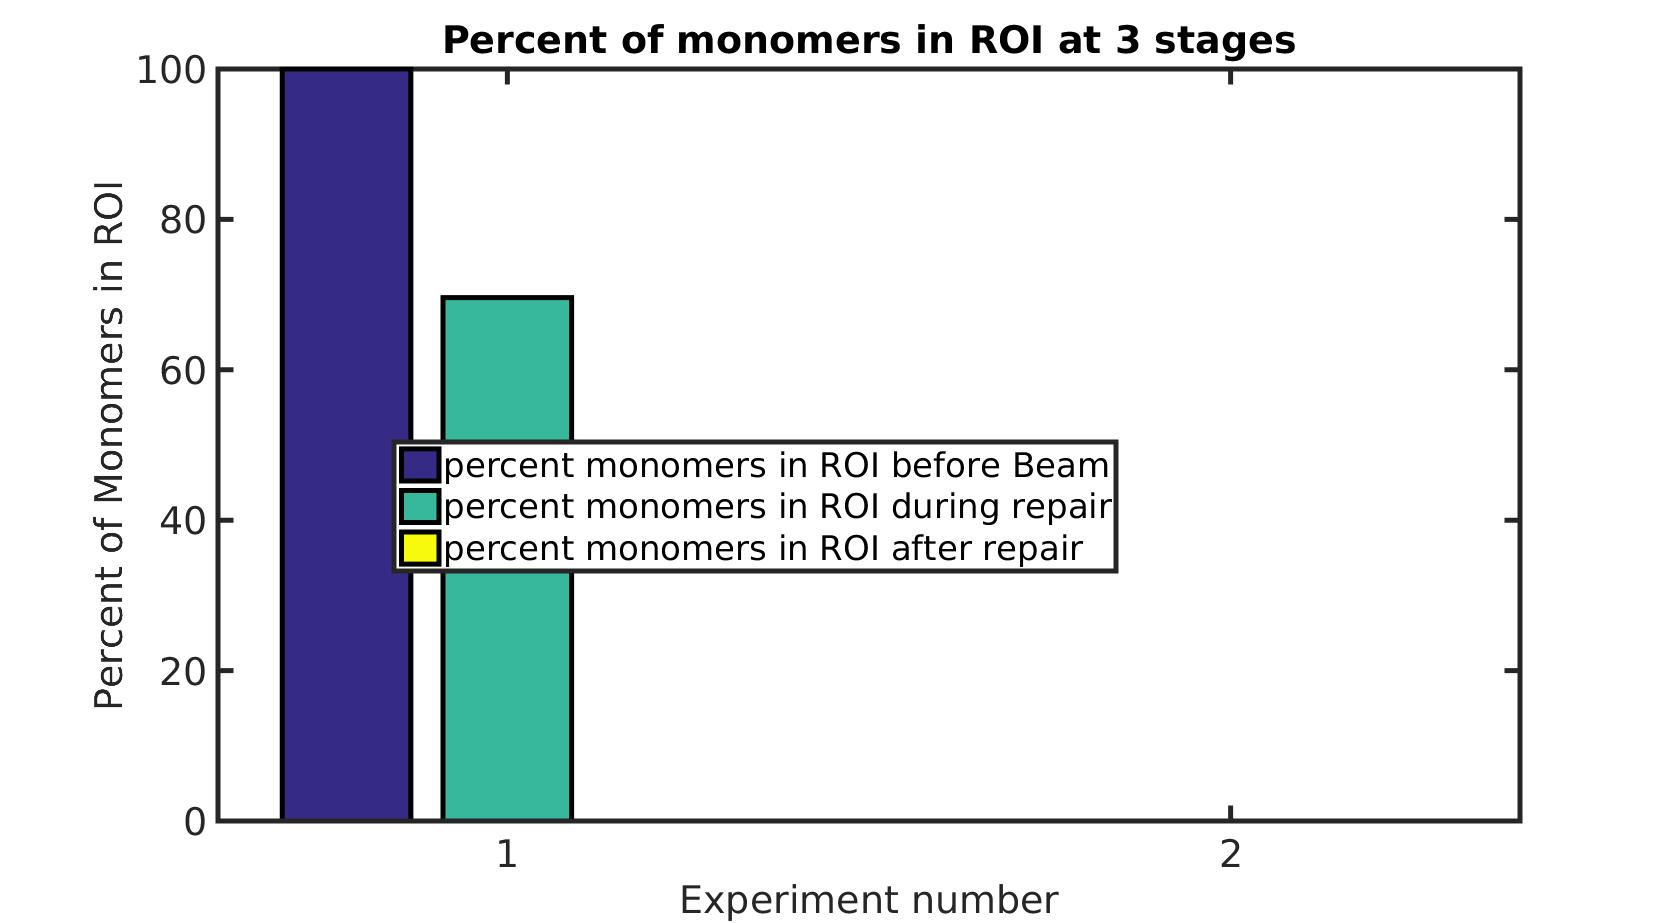
\includegraphics[width=0.5\linewidth, height=0.3\textheight]{Images/ExludeAroundDamagedMonomers/BreakDamagedCrosslinks/testExpansion/percentOfMonomersInROI}
	\caption{\tiny{\textbf{The number of monomers in ROI (left) and the percent of monomers (right) in the ROI. As can be seen, a 30\% loss is achieved with $R_e=0.68$.}}}
	\label{fig:meannumberOfMonomersInROI}
	\end{figure}
	 Although the loss reached 30\%, we should not worry about this too much because we can adjust the rate of the loss using the exclusion parameters, to fit experimental observations 15 minutes post UVC.
	 
   \textbf{\large{constant of exclusion $k_e$}}\\
   In all experiments we keep the exclusion constant equal $k_e=\frac{2k_bT}{b^2}$\\ 
   
   \subsubsection{Length of DNA in ROI}
   The polymer model we use describes the chromatin as beads connected by springs. Because during repair stage, after UVC, we stop diffusion and let the chain relax, all bonds (springs) reach roughly a constant minimal allowed length, making the chain effectively a bead-spring model. In later stages, when nucleusomes will be placed on bonds and will have dynamics, we will expect the loss after UVC to be 40\%. That means nucleusomes should slide or be displaced by some mechanism along the contour of the polymer away from damage sites (not including on cross-links). In the model we make for the chromatin, several nucleusomes will be grouped together and moved after UVC. due to this grouping, we should prevent unrealistic crowding of nucleosomes on a single bond. Therefore, the expected number of nucleosomes loss post UVC will be a function of the resting length of the bonds, the number of monomers damaged, and the nucleosome crowding limit we set. Although we expect a correlation between monomer loss and bond length in the ROI, we set out to examine what is the total length of bonds in the ROI after UVC. 
   This should give us an indication of how many nucleosomes are displaced post UVC based on the allowed density of nucleosomes in a bond. 
   
   Interestingly, although the bond length in ROI and the number monomers are correlated, the percentages of loss are different. We set experiments in which 80\% connectivity is chosen and we vary the radius of exclusion from 0.2 to $\sqrt{2}/2$.  While monomer loss reaches 20\%, the total bond length losses up to 5\%. This phenomena is caused by the fact that the boundaries of the ROI are being densely populated with non damaged monomers after UVC and the exclusion area is effective in a finite range. That is, monomers are being pushed away from damaged monomers but stop when they are out of reach of the pushing force. In contrast, bonds are not completely affected
   
   

  \subsection{Summary of Damage Stage}
	 We have examined several scenarios in which a UVC beam was shot through the center-of-mass of a polymer. As a result, an expansion of the polymer is seen in the damage region. To simulate this expansion, we have assigned bending elasticity to either one of the four groups of monomers: the damaged monomers (and their nearest neighbors) the non-damaged monomers, the non-damaged monomers found in the UVC beam, and both the damaged and non-damaged alike. 
	 
	 It was observed that when the damaged monomers were assigned bending elasticity post UVC, an uncontrolled expansion has occurred (measured by the mean radius around the damaged monomers' center of mass). To keep the polymer from expanding, we have randomly added cross-links between pairs of monomers. The degree of cross-linking was determined by percentages of added connectivity in relation to the total number of monomers. These cross-links were either broken or kept post UVC, both scenarios have been examined. 
	 
	 Keeping all cross-links post UVC indeed stopped the expansion of the damaged monomers. However, instead of loss in the repair region, the polymer collapsed onto itself and an increase in the number of monomers was observed at the end of simulation. Similarly, breaking cross-links for damaged monomers showed and increase in radius of expansion and no significant lose of monomers was seen at the end of simulation. However, we favor the scenario by which damaged cross-links were broken post UVC, which is much more plausible in biological setting. 
	 
	 Breaking cross-links from damaged monomers agrees with observations by which repair mechanism loosens the connection between molecules such as CTCF and cohesin and makes the damage region more flexible. This flexibility in the damaged can be thought of the result of crowding of repair mechanism, recruited to the damaged zone. Indeed, by breaking the cross-links of damaged monomers the mean distance between monomers increases, which can be seen as the result of the presence of repair mechanism related proteins in the vicinity of each damaged monomer. 
     
     It was shown that when bending is assigned to the damaged monomers, the radius of expansion is larger than that of the non-damaged ones. Because we determine the region of interest according to the damaged monomers' radius of expansion, it then shows immediately that there could be no loss of monomers in the region, since it include most of them (both damaged and non-damaged). In contrast, assigning bending to the non-damaged monomers (while keeping non-damaged cross-links, and breaking damaged cross-links) proved to supply exactly the result we have anticipated: the damaged monomers redistribute, since the cross-links are broken), the non-damaged monomers leave the ROI determined by the damaged monomers, and so allow a reduction of 20\% (if the cross-linking percentage exceeds 70\%). Assigning bending elasticity to the non-damaged can be justified by the fact that repair protein, who enter the region after UVC damage, push aside all irrelevant (non-damage) DNA.
     
     In addition, a second feasible model has proven to agree with experimental observations. The model, as its former, includes random cross-linking of monomers and breaking the damaged cross-links after UVC. However, instead of assigning bending elasticity force, a circular area around each damaged monomer is used for exclusion of other monomers by mean of harmonic force. This was made to mimic the recruitment, binding and crowding around damaged site, by repair mechanism related proteins.
     
          
     Which ever one of the two model represents real experiments is left for biological validation. however, the principle remains similar in both, the non damaged monomers are the mobile one and by their dynamics post UVC are responsible for the 20\% loss seen n experiments. The damaged monomers (regions) remain within the repair zone and are less mobile due to the attachment of repair proteins. 
          
\section{Microscopic Description of DNA and Nucleusome Loss}
\subsection{1D model of nucleosome sliding and chromatin expansion}\label{subsection:1dModelOfNucleosomeSliding}
   To provide a microscopic description of nucleosome loss in the ROI, we need to state some observations and assumptions:
   \begin{enumerate}
   	\itemsep0em
   	\item histone- wrapped DNA is 3 times more probable to be damaged by UV than the linker DNA;
   	\item repair mechanism presence indicate damage site;
   	\item the repair zone is roughly circular;  
   	\item repair must occur on a naked DNA, with no histones on it; 
   	\item histone sliding on a damage site can be slided again to expose the damage site;
   	\item histones can be pushed any distance;
   	\item histones can slide over damage sites (since they have damages on the DNA that is wrapped around them);
   	\item length of linker DNA=50bp, length of histone-wrapped DNA=150bp;
   	\item we consider nuclesome to be the linker + the histones as a unit.   
   \end{enumerate}
   With these assumptions and observations, I'll present a simplified 1D model which accounts for 40\% loss of histones, and 20\% loss of DNA, in a region expanding $\beta$ times its initial size. 
   
   We start with a 1D model of a DNA strand with nucleosomes embedded in it. The leftmost point of the strand will be the origin. In this model, a UV beam damages a portion of size $L$ of the strand containing $N$ nucleosomes. Assume the rightmost damage point,$S$, is located at $L$. According to the assumption, repair can take place only on naked DNA. Therefore, in order to repair all damages, the repair proteins need to slide histones away from high concentration of damage sites. Assuming the focal point of the beam is above the origin, sliding direction will be to the right. From symmetry arguments, a mirror situation can be to extended to the left of the beam focal point.     
   
   The first principle to take into account is that sliding histones over any point of the DNA displaces that point several bp to the right (Figure \ref{fig:histoneSlidingSingle}). The actual distance it is displaced depends on the number of bp wrapped around each histone. It is important to note that this displacement is not a displacement of the point on the actual DNA, but rather measured by the aerial distance from the origin to the point. This displacement is caused by the sliding histones over the DNA.
   
   Assume now that the repair proteins have slided enough histones to reach a geometrical arrangement such that al damage sites are exposed. If we look at the rightmost damage point ,$S$, initially located at a distance of $L$ from the origin, then as a result of histones sliding, $S$ has been displaced from $L$ to $\beta L$. 
   
   For the point $S$ to reach $\beta L$ we need to displace $S$ a distance equivalent to of $(\beta-1)L$. Assume that a single nucleosome units (linker + histone) occupies a length of $\alpha_1$, and with each sliding of the histone over a point, we displace this point a length fo $\alpha_2$. The ratio $\alpha_1/\alpha_2 =\alpha$ will be used in the calculation. Then, The number of times we have to slide a histone over the point $S$ is thus $(\beta-1)N\alpha$.
   The number also indicates the number of histones transfered from the left to the right side of the point $S$ as it is being translated towards $\beta L$.
   In the region $\beta L$ we initially have $\beta N$ nucleosomes. After the point $S$ has reached $\beta L$ the region contains $N-(\beta-1)N$ nucleosomes plus the amount crossing over from left to right of $S$. 
   
   Since the point $S$ is a damage site, we expect to find tagged repair proteins around it, and so also at $\beta L$. Therefore, the  boundaries of the ROI, which are determined by presence of repair protein, will be at $\beta L$ with the point $S$. 
   
   The percent of DNA loss from the ROI due to sliding is thus 
   \begin{equation}
   \frac{(\beta-1)}{\beta}
   \end{equation}
   All nucleosomes to the right of the point $S$ are lost, and in addition all nucleosomes which were slided from left to right of $S$ are lost. This brings the total percentage of nucleosome loss to 
   \begin{equation*}
   \frac{(\beta-1) +\alpha(\beta -1)}{\beta}= \frac{(\alpha+1)(\beta -1)}{\beta}
   \end{equation*}
   which is independent of $N$.
   
   Experimental result show 20\% of DNA loss, therefore we equate the loss of DNA to 0.2 
   \begin{equation*}
   \frac{(\beta -1)}{\beta}=0.2, \quad \Rightarrow \beta = 1.25
   \end{equation*}     
   Histone loss is 40\%, which immediately gives $\alpha =1$.
   
   The value $\alpha=1$ has geometrical meaning and is the ratio of the distance we displace a point to the length of DNA wrapped on a histone. 
   
   Experimental observations show a growth of 1.7 in the radius of expansion. This is in no agreement with $\beta=1.25$ found in the 1D analytical calculation. We therefore have to incorporate information related to the spatial organization of the DNA. 
   
   
   \begin{figure}
   	\centering
   	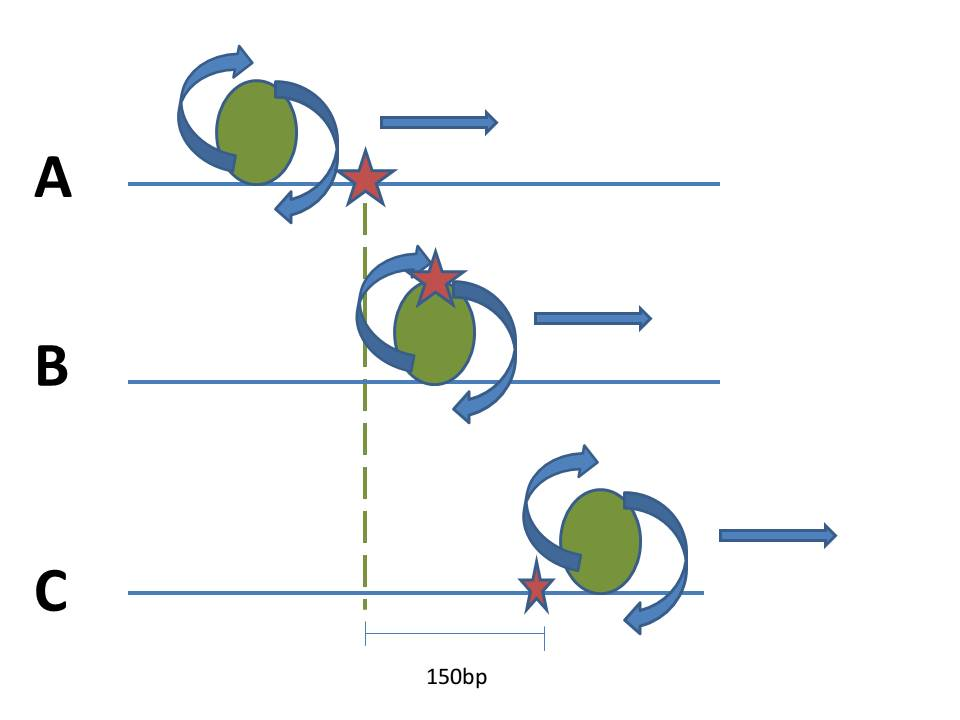
\includegraphics[width=0.7\linewidth]{histoneSlidingSingle}
   	\caption{{Three time points during a displacement of damage site (red star) caused by histone rolling. The displacement of the damage site is equivalent to the length of DNA wrapped on a histone. A displacement is relative to some reference point, like the origin, and does not refer to an actual motion on the DNA}}
   	\label{fig:histoneSlidingSingle}
   \end{figure}
   
   \begin{figure}
   	\centering
   	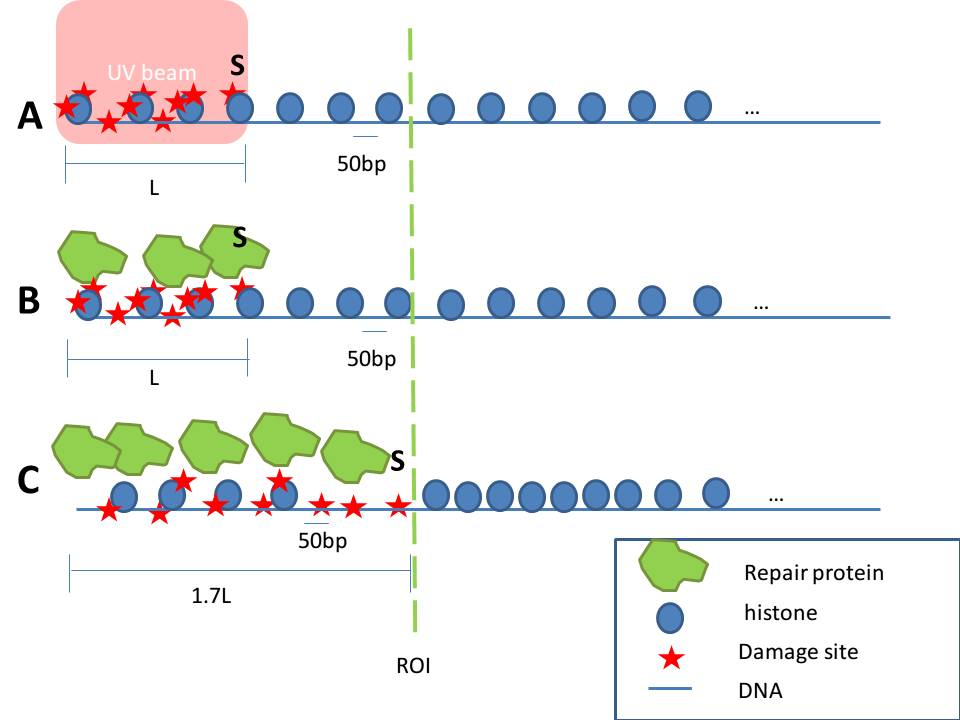
\includegraphics[width=0.7\linewidth]{histoneSlidingMulti}
   	\caption{Expansion of the ROI due to nucleusome rolling. \textbf{A}. a UV beam (transparent red) damages DNA, with the point $S$ being the rightmost damage site \textbf{B}. Repair proteins (green polygons) are recruited to the damage site and start to expose the DNA in order the repair damages. \textbf{C}. Sliding the nucleosomes to the right in order to expose damage sites, translates the point $S$ to the right until $S$ reached $\sqrt{3}L$. Repair proteins are present at the new location. The presence of repair proteins in $\beta L$ indicates the ROI's boundary (vertical dashed green line). All DNA and histones to the right of $S$ are lost}
   	\label{fig:histoneSlidingMulti}
   \end{figure}
   
\subsection{2D model- incorporating experimental observations}\label{subsection:2dModel}
To generalize the simple 1D model into 2D we have to take into account the geometry of the problem. In the 1D model expansion of the damage zone occurs by sliding alone. As seen there, the radius of expansion required to reach 40\% loss of nucleosome signal is only 1.25 times the initial UV beam radius. However, in experimental results we see an expansion of the size 1.7. We then have to attribute some of the expansion to repair protein crowding in the repair region. The contribution of crowding will be explored in this subsection. 

We start by observing the marked patch of nucleosomes at time 0 and 15 minutes post UVC. The patch area at time 0 is 20$\mu m^2$, which yields a radius of 2.52$\mu m$. After expansion at 15 minutes post UVC, the patch radius grows by 30\% to 3.28$\mu m$ (measured manually). We further assume that there is no loss in the signal of marked nucleosomes during 15 minutes post UVC stemming from the patch. The absolute expansion of the patch is $3.28-2.52=0.756\mu m$. This is roughly equivalent to the radius of expansion of the damage zone, which is 0.73 $\mu m$. We interpret this observation as the non compressibility of the chromatin. All chromatin pushed by crowding from the damage zone, are pushing further away to expand the patch equivalently. In this sense, we cannot determine the relative contribution of crowding and histone sliding to the expansion of the patch. 

From the graphs of concentric old H3.3 signal around the damage site, we now calculate the loss/gain of signal relative to the signal in the patch at time 0. The signal in the patch will from as a reference to the signal 15 minutes post UVC. dividing the signal at time 15 with the signal at time 0 as a function of the radius from the center, we obtain to following graph

\begin{figure}[H]
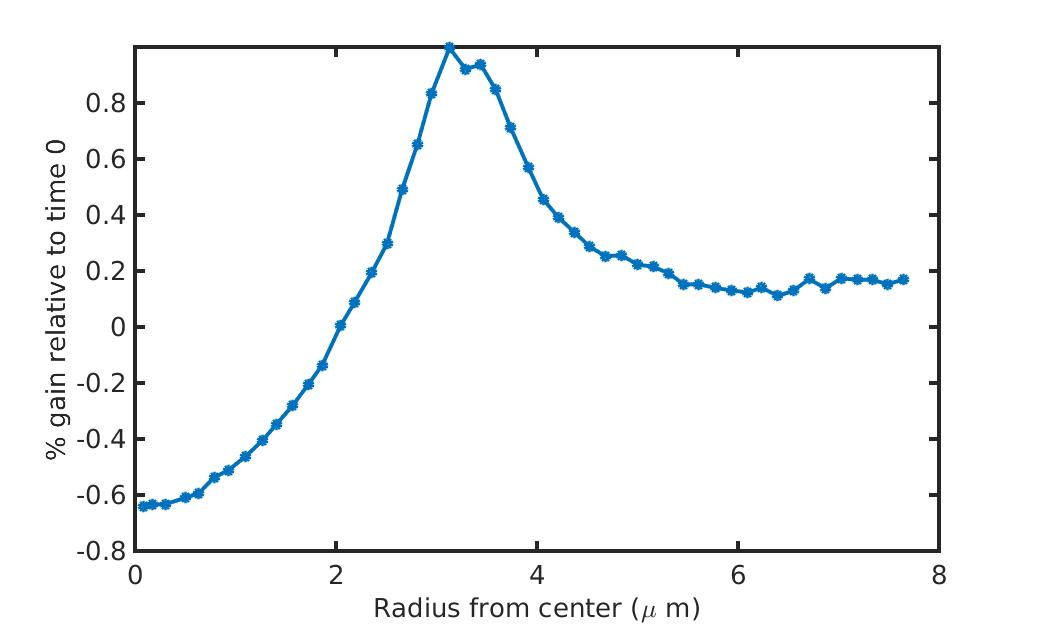
\includegraphics[width=0.5\linewidth, height=0.3\textheight]{Images/patchExpansion/relativeGainNucleosomesConcentric}
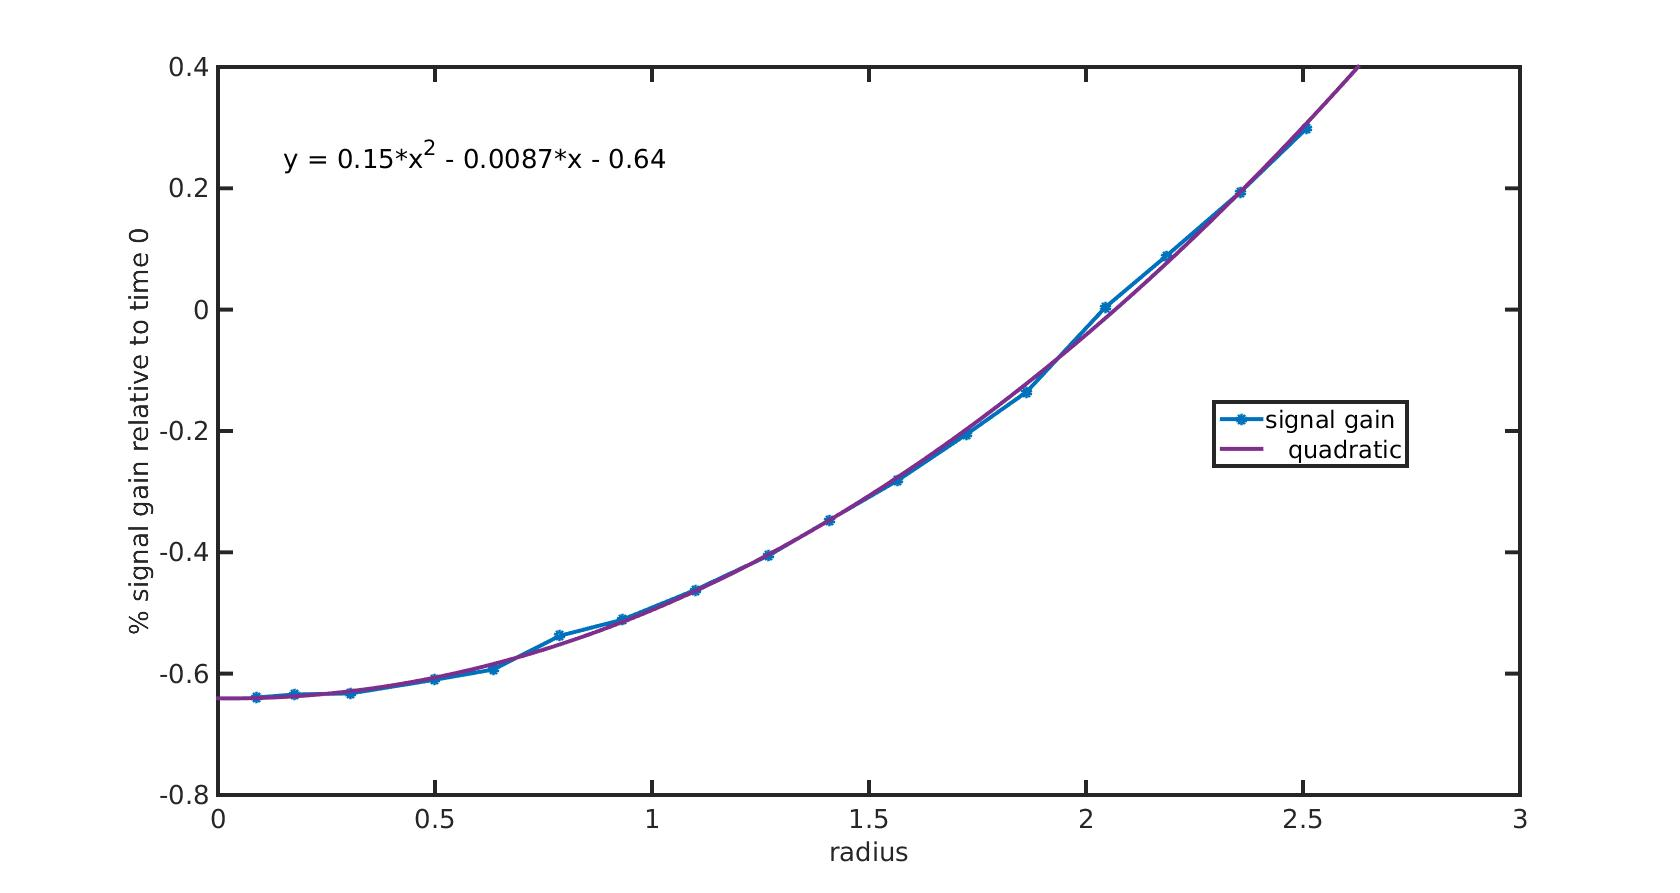
\includegraphics[width=0.5\linewidth, height=0.3\textheight]{Images/patchExpansion/nucleosomeSignalGainConcentricFit}
\caption{}
\label{fig:relativeGainNucleosomesConcentric}
\end{figure}

We now fit a quadratic function to this graph up to radius 2.52, which is the initial radius of the patch. This is done because for higher radii the signal is not reliable and includes gain of signal in areas that were initially outside the patch. The quadratic fit has the form 
\begin{equation*}
y(r)=0.15r^2-0.0087r-0.64
\end{equation*}
The function $y(r)$ represent the gain and loss in percentages due to both pushing and sliding of DNA and nucleosomes. 

Since the precentages are taken from growing concentric rings, which include higher quantity of nucleosomes with ting size, we have to calculate the actual distribution of DNA and nucleosomes in each ring. For this end we multiply the gain-loss function $y(r)$ with the amount of material expected in each concentric ring. The DNA is thought to be uniformly distributed in the nucleus prior to UVC and with uniform density. 

Taking rings separated  $dr$ apart and assuming the circle of radius  $1 \mu m$ contains $N$ particles, then the material between the rings of $r$ and $r+dr$ contains  
\begin{equation*}
F(r)dr = 0.5N\left((r+dr)^2- r^2\right)=Nrdr+(dr)^2
\end{equation*}
the term $dr ^2$ vanishes when $dr$ is small.
From each one of the concentric rings we lose a percentage of material following $y(r)$ in Figure \ref{fig:relativeGainNucleosomesConcentric}. Therefore, the amount of material remaining 15 minutes post UVC between $r$ and $r+dr$ is
\begin{equation*}
F(r)(y(r)+1)dr
\end{equation*}
Using this function we now search for the radius $R$ for which $\gamma$ of the initial material remains in the circular region enclosed between 0 and $R$. That is 

\begin{equation*}
\frac{\int_0^RF(r)(y(r)+1)dr}{\int_0^RF(r)dr} =\gamma
\end{equation*} 

Plugging-in  $F(r)=r,y(r)=ar^2 +b^r +c$ and performing integration, 
\begin{equation*}
\int_0^R r(ar^2 +br+c +1-\gamma)dr =0
\end{equation*}
we obtain a forth-order polynomial  in $R$ which has the same roots of the second order polynomial 
\begin{equation*}
\frac{aR^2}{4} +\frac{bR}{3} +\frac{c+1-\gamma}{2}
\end{equation*}
Plugging-in the values $a=0.15, b=-0.0087,c=-0.64, \gamma=0.6$, we find the roots are 
\begin{equation*}
R_1=1.8279, \quad R_2= -1.7506
\end{equation*}

The positive root indicates that with the mechanism in the function $y(r)$, a 40\% loss is seen at a distance of 1.8279 from the center, which is close to the observed value of $\sqrt{3}$ for the ROI boundary. We treat this result as being in agreement with the observations and in the range of acceptable measurement error.

The mechanism describing loss and gain, namely $y(r)$, can also be used to predict the distance $R$ for which the loss of DNA and histones is balanced, in the sense that all signal loss from the ROI is gained at the periphery of the region. We therefore set $\gamma =1$ and calculate
\begin{equation*}
\int_0^R F(r)y(r)dr = 0
\end{equation*}
which results in a second-order polynomial with roots 
\begin{equation*}
R_1=2.906, \quad R_2=-2.882
\end{equation*}.

Taking the positive root, the predicted radius for which the loss is balanced is at $R=2.906$. In practice, the patch expands to $3.28$, which give an unexplained difference fo $0.32$. 

To explain the observed difference we need to elaborate on the gain-loss mechanism given by the function $y(r)$. According to our assumptions, the function $y(r)$ describes the loss of both DNA and histones by two sub-mechanisms; one caused by crowding of repair proteins in the ROI which creates pushing of material on one end, and straightening damaged DNA on the other; and a second sub-mechanism due to sliding of histones to expose the damaged DNA for repair activity. The second sub-mechanism is explained in sub-section \ref{subsection:1dModelOfNucleosomeSliding}.  

We assume that by the mechanism of pushing and straightening DNA in preparation for repair, no DNA packing is caused. In contrast, the mechanism of histone sliding packs both histones and DNA. It is important to note that the pushing mechanism is active during histone sliding but not necessarily to the converse; crowding and pushing is always present during expansion, whereas sliding can be alternatively activated. 

We can now explain the 0.32 difference in the predicted and observed patch expansion by the activity of sliding mechanism. 
If both mechanisms would have been active continuously throughout expansion, the material loss would have been balanced at distance $2.906$ from the center. However, expansion of the patch continuous up to 3.28. This means that sliding is only active in $(\sqrt{3}-1-0.32)/(\sqrt{3}-1) =0.56$  parts of the way (or time, alternate or continuously throughout expansion stage) while pushing mechanism is continuously active.




 






 
\section{DNA repair}
	
\end{document}